
\documentclass[
	a4paper, 
	fontsize=10pt,
	twoside=true, 
	%open=any,
	%chapterentrydots=true, 
	numbers=noenddot, 
]{kaobook}

\ifxetexorluatex
	\usepackage{polyglossia}
	\setmainlanguage{spanish}
\else
	\usepackage[spanish]{babel} 
\fi
\usepackage[spanish]{csquotes}	

\newcommand{\framedtext}[1]{%
\par%
\noindent\fbox{%
    \parbox{\dimexpr\linewidth-2\fboxsep-2\fboxrule}{#1}%
}%
}

\usepackage{blindtext}
%\usepackage{showframe} % Uncomment to show boxes around the text area, margin, header and footer
%\usepackage{showlabels} % Uncomment to output the content of \label commands to the document where they are used

% Load the bibliography package
\usepackage{kaobiblio}
\addbibresource{main.bib} % Bibliography file

% Load mathematical packages for theorems and related environments
\usepackage[framed=true]{kaotheorems}

% Load the package for hyperreferences
\usepackage{kaorefs}

%%%%%%%%%%%%%%%%Paquetes%%%%%%%%%%%%%%%%%%%%%%%
\usepackage{witharrows}
\usepackage{physics}
%%%%%%%%%%%%%%%%%%%%%%%%%%%%%%%%%%%%%%%

\graphicspath{{../Images}{images/}} % Paths in which to look for images

\makeindex[columns=3, title=Alphabetical Index, intoc] % Make LaTeX produce the files required to compile the index

\makeglossaries % Make LaTeX produce the files required to compile the glossary

    
    \newglossaryentry{computer}{
      name=computer,
      description={is a programmable machine that receives input, stores and manipulates data, and provides output in a useful format}
    }

    % Glossary entries (used in text with e.g. \acrfull{fpsLabel} or \acrshort{fpsLabel})
    \newacronym[longplural={Frames per Second}]{fpsLabel}{FPS}{Frame per Second}
 % Include the glossary definitions

\makenomenclature % Make LaTeX produce the files required to compile the nomenclature

% Reset sidenote counter at chapters
\counterwithin*{sidenote}{chapter}

\begin{document}

\titlehead{Apuntes de Mecánica Teórica}
\subject{Mecánica Teórica}

\title[]{Título}
\subtitle{Profesora Maria del Prado Castillo}

\author[]{}

\date{\today}

\publishers{An Awesome Publisher}

\frontmatter

\makeatletter
\uppertitleback{\@titlehead}

\makeatletter
\uppertitleback{\@titlehead} % Header

\lowertitleback{
  \textbf{Aviso}\\
  Estos apuntes son basicamente una recopilación de los libros que usa Prado en clase y con algunas anotaciones, la mayoria de cosas son literales de los libros y traducidas y poco más salvo algunas notas que he ido cogiendo. 

  Hay mucho más de lo que hace falta.


}
\makeatother

\maketitle

\begingroup % Local scope for the following commands

% Define the style for the TOC, LOF, and LOT
%\setstretch{1} % Uncomment to modify line spacing in the ToC
%\hypersetup{linkcolor=blue} % Uncomment to set the colour of links in the ToC
\setlength{\textheight}{230\hscale} % Manually adjust the height of the ToC pages

% Turn on compatibility mode for the etoc package
\etocclasstocstyle % "toc display" as if etoc was not loaded
\etocstandardlines % "toc lines" as if etoc was not loaded

\tableofcontents % Output the table of contents

\listoffigures % Output the list of figures

% Comment both of the following lines to have the LOF and the LOT on different pages
\let\cleardoublepage\bigskip
\let\clearpage\bigskip

\listoftables % Output the list of tables
\printglossary
\endgroup

%----------------------------------------------------------------------------------------
%	MAIN BODY
%----------------------------------------------------------------------------------------

\mainmatter % Denotes the start of the main document content, resets page numbering and uses arabic numbers
\setchapterstyle{kao} % Choose the default chapter heading style



\pagelayout{wide}

\addpart{Mecánica Lagrangiana y Hamiltoniana}

\pagelayout{margin}
\setchapterpreamble[u]{\margintoc}
\chapter{Mecánica Lagrangiana}
\labch{Part}

\section{Dinámica Lagrangiana}
En este capítulo mostramos cómo se pueden reescribir las ecuaciones de movimiento en la variedad de configuración adecuada, de forma que las restricciones se tengan en cuenta desde el principio. El resultado es la formulación lagrangiana de la dinámica (las ecuaciones de movimiento se denominan entonces ecuaciones de Lagrange). Hay que subrayar que el contenido físico de las ecuaciones de Lagrange es el mismo que el de las de Newton. Pero además de ser lógicamente más atractiva, la formulación de Lagrange tiene varias ventajas importantes.

Quizá la primera ventaja evidente es que la formulación lagrangiana es más fácil de aplicar a sistemas dinámicos distintos del más simple. Además, pone de manifiesto la conexión entre las leyes de conservación e importantes propiedades de simetría de los sistemas dinámicos. De gran importancia es que las ecuaciones de Lagrange pueden derivarse de un principio variacional, un método que resulta ser extremadamente general y aplicable en muchas ramas de la física. Una de las razones para estudiar mecánica clásica es comprender la formulación lagrangiana, ya que muchas ecuaciones de la física se formulan convencionalmente en términos lagrangianos y muchas leyes de conservación se entienden también en términos lagrangianos, a través de su conexión con las simetrías.

\subsection{Espacio de configuración}
(54-70)

En esta sección cambiamos las coordenadas cartesianas por otras más útiles para tratar sistemas dinámicos. Las nuevas coordenadas se eligen de un modo que depende del sistema dinámico concreto para el que se van a utilizar (pero se denominan, no obstante, coordenadas generalizadas); se adaptan a ese sistema y son coordenadas más o menos naturales para él. Las propiedades del sistema que determinan la elección son geométricas: son el número de libertades y la forma, o topología, de la región en la que el sistema es libre de moverse (por ejemplo, si es una esfera o un plano inclinado). Esta región está determinada por las restricciones impuestas sobre el sistema; se llama el espacio de configuraciones $\mathbb{Q}$. Las nuevas coordenadas, llamadas $q^{\alpha}$, estarán en $\mathbb{Q}$, y su número será el número de libertades, que es también la dimensión de $\mathbb{Q}$. En esta sección hacemos dos cosas 
\begin{enumerate}
  \item Explicar la idea del colector de configuración
  \item Describir el cambio de las coordenadas cartesianas a las $q^{\alpha}$
\end{enumerate}

\subsection{Lagrangianos equivalentes}



Aunque la función Lagrangiana determina las ecuaciones de movimiento de manera única, las ecuaciones de movimiento no determinan la Lagrangiana de manera única. Es decir, dos Lagrangianas que son diferentes pueden conducir a ecuaciones de movimiento que son las mismas. Por ejemplo, sea $L_{1}$ y $L_{2}$ dos funciones Lagrangianas tales que las ecuaciones de movimiento obtenidas de ellas son exactamente las mismas. Entonces se puede demostrar que existe una función $\Phi$ en $\mathbb{Q}$ tal que 

\[
L_{1}-L_{2}=\frac{d \Phi}{d t}.
\]

Para probar esta afirmación, debemos explicar lo que se entiende por "exactamente las mismas". 
\begin{proof}
  Para este propósito, consideremos las $2 n$ funciones $\Lambda_{j \alpha}$, donde $j=1,2$, y $\alpha=1, \ldots, n$, definidas por

\[
\frac{d}{d t} \frac{\partial L_{j}}{\partial \dot{q}^{\alpha}}-\frac{\partial L_{j}}{\partial q^{\alpha}} \equiv \Lambda_{j \alpha}(q, \dot{q}, \ddot{q}, t)
\]

de modo que las ecuaciones de Lagrange se pueden escribir como 

\[
\Lambda_{j \alpha}(q, \dot{q}, \ddot{q}, t)=0.
\]

Entonces, decir que las ecuaciones de movimiento son exactamente las mismas es decir que las dos funciones son iguales. En otras palabras, 

\[
\Lambda_{1 \alpha}=\Lambda_{2 \alpha} \tag{2.30}
\]

identicamente, para cada $\alpha$. Ahora procedemos a probar la afirmación, pero solo para un grado de libertad (es decir, para $n=1$), dejando el caso general para el Problema 4. Para $n=1$, el índice $\alpha$ puede ser eliminado de las ecuaciones. Escribimos $\psi=L_{1}-L_{2}$. Entonces, la Ec. (2.29) se puede usar para escribir (2.30) en la forma 

\[
\Lambda_{1}-\Lambda_{2} \equiv \frac{\partial^{2} \psi}{\partial \dot{q}^{2}} \ddot{q}+\frac{\partial^{2} \psi}{\partial q \partial \dot{q}} \dot{q}+\frac{\partial^{2} \psi}{\partial \dot{q} \partial t}-\frac{\partial \psi}{\partial q}=0 \tag{2.31}
\]

Debido a que $L_{1}$ y $L_{2}$ son funciones solo de $q, \dot{q}$ y $t$, también lo es $\psi$, y por lo tanto el único lugar donde $\ddot{q}$ aparece en (2.31) es donde se ve multiplicando el primer término. Pero (2.31) debe ser cierto para todos los valores de $q, \dot{q}, \ddot{q}, t$. Por lo tanto, el coeficiente de $\ddot{q}$ debe anularse: $\frac{\partial^{2} \psi}{\partial \dot{q}^{2}}=0$. Esto significa que $\psi$ es lineal en $\dot{q}$:

\[
\psi=\dot{q} F(q, t)+G(q, t) \tag{2.32}
\]

Esto y un poco de álgebra pueden usarse para transformar (2.31) en 

\[
\frac{\partial F}{\partial t}-\frac{\partial G}{\partial q}=0 \tag{2.33}
\]

Esto es solo la condición de integrabilidad para el par de ecuaciones 

\[
F=\frac{\partial \Phi}{\partial q} \quad \text{y} \quad G=\frac{\partial \Phi}{\partial t} \tag{2.34}
\]

Es decir, (2.33) es la condición de que exista una función local $\Phi(q, t)$ que haga posible escribir $F$ y $G$ localmente en la forma de (2.34). Cuando se escriben de esta manera, (2.32) se convierte en 

\[
\psi=\dot{q} \frac{\partial \Phi}{\partial q}+\frac{\partial \Phi}{\partial t} \equiv \frac{d \Phi}{d t}
\]

como se afirmó.
\end{proof}

La énfasis en la localidad aquí es para advertir al lector que puede no ser posible encontrar una función univaluada $\Phi(q, t)$ en todo $\mathbb{Q}$. Tales cuestiones se discutirán más a fondo más adelante.

Lo que acabamos de probar (o más bien lo que se prueba en el Problema 4) significa que si una Lagrangiana se cambia al agregar la derivada temporal de una función, las ecuaciones de movimiento no se verán alteradas. Sin embargo, esto no significa que las Lagrangianas que producen la misma dinámica deben diferir necesariamente por una derivada total en el tiempo. Por ejemplo, 

\[
L_{a}=\dot{q}^{1} \dot{q}^{2}-q^{1} q^{2} 
\]

y 

\[
L_{b}=\frac{1}{2}\left[\left(\dot{q}^{1}\right)^{2}+\left(\dot{q}^{2}\right)^{2}-\left(q^{1}\right)^{2}-\left(q^{2}\right)^{2}\right]
\]

producen la misma dinámica, pero no difieren por una derivada total en el tiempo.



\subsection{Coordenadas independientes}


Las ecuaciones de Lagrange se derivaron sin especificar de ninguna manera los coordenadas generalizadas particulares utilizadas en $\mathbb{Q}$, y por lo tanto, son válidas en un sistema de coordenadas tanto como en otro. Esta es una propiedad importante y útil de la formulación lagrangiana (ver la Sección 2.2.4 para un ejemplo de su utilidad). Para observarlo en detalle, sea $q^{\prime 2}(q, t)$ un nuevo conjunto de coordenadas generalizadas, en cuyo caso las funciones deben ser invertibles: existen $q^{\omega}(q^{\prime}, t)$. Lo que esto significa físicamente es que es posible escribir las trayectorias de las partículas en términos de $q^{\prime \alpha}$ así como en términos de $q^{\alpha}$, y cuando se conocen en términos de un conjunto, se pueden calcular en términos del otro. Cuando se conocen los $q^{\alpha}(q^{\prime}, t)$, también se conocen los $\dot{q}^{\alpha}(q^{\prime}, \dot{q}^{\prime}, t)$:

\begin{DispWithArrows}[displaystyle, format=c]
\dot{q}^{\alpha}\left(q^{\prime}, \dot{q}^{\prime}, t\right)=\frac{\partial q^{\alpha}\left(q^{\prime}, t\right)}{\partial q^{\prime \beta}} \dot{q}^{\prime \beta}+\frac{\partial q^{\alpha}\left(q^{\prime}, t\right)}{\partial t} \tag{2.35}
\end{DispWithArrows}


La Lagrangiana es una función de $2 n+1$ variables: las $n$ coordenadas generalizadas, sus $n$ derivadas temporales, y el tiempo. Esto significa que $L$ asigna un número real (el valor de la función) a cada conjunto de $2 n+1$ números (los valores de las variables). Pero el conjunto de $2 n+1$ números describe el estado físico del sistema dinámico. Por lo tanto, la función Lagrangiana asigna un número real no a cada conjunto de $2 n+1$ números, sino al estado físico en sí. Cuando se realiza una transformación de coordenadas, el mismo estado físico del sistema se describe mediante un conjunto diferente de $2 n+1$ números. Dado que el estado no cambia, la función Lagrangiana debe asignar el mismo valor real a este conjunto transformado de $2 n+1$ números.

Ahora lo hacemos explícito matemáticamente. Suponga que se da una función Lagrangiana $L(q, \dot{q}, t)$ en las coordenadas originales, sin primar. Se puede escribir en términos de las coordenadas primadas simplemente sustituyendo las expresiones conocidas para $q^{\alpha}$ y $\dot{q}^{\alpha}$ en términos de $q^{\prime \beta}$ y $\dot{q}^{\prime \beta}$. El resultado será una nueva función Lagrangiana (transformada) $L^{\prime}$ de las coordenadas primadas, diferente de $L$. Es decir, $L^{\prime}\left(q^{\prime}, \dot{q}^{\prime}, t\right)$ está definida por

\begin{DispWithArrows}[displaystyle, format=c]
L^{\prime}\left(q^{\prime}, \dot{q}^{\prime}, t\right) \equiv L\left(q\left(q^{\prime}, t\right), \dot{q}\left(q^{\prime}, \dot{q}^{\prime}, t\right), t\right) \equiv L(q, \dot{q}, t) \tag{2.36}
\end{DispWithArrows}


la igualdad surge de lo que se ha dicho: las variables primadas y no primadas describen el mismo estado físico del sistema. Entonces, como se muestra en el Problema 3, las ecuaciones de Lagrange (2.28) implican

\begin{DispWithArrows}[displaystyle, format=c]
\frac{d}{d t} \frac{\partial L^{\prime}}{\partial \dot{q}^{\prime \prime}}-\frac{d L^{\prime}}{d q^{\prime \alpha}}=0 \tag{2.37}
\end{DispWithArrows}


Debido a que esta ecuación y (2.28) son igualmente válidas, se dice que las ecuaciones de Lagrange son independientes de las coordenadas (o covariantes bajo transformaciones de coordenadas). Pero entonces, estas ecuaciones están haciendo una afirmación que no depende de las coordenadas, y los específicos $q^{\alpha}$ o $q^{\prime 2}$ que aparecen en ellas desempeñan un papel no esencial, completamente auxiliar. Debería entonces haber una manera de escribir estas ecuaciones diferenciales sobre el conjunto de configuraciones de tal manera que las coordenadas no aparezcan.



\todo{Aunque realmenete luego siempre volvemos a las coordenadas espaciales en la práctica}
\subsection{Condición Hessiana}

Tanto en las formulaciones de Lagrange como en las de Newton, las ecuaciones del movimiento son de segundo orden. Estas ecuaciones describen cómo evoluciona el estado de un sistema prescribiendo la aceleración basada en el estado actual, es decir, la posición y la velocidad del sistema. La integración de estas ecuaciones, comenzando desde las condiciones iniciales, nos permite determinar el comportamiento del sistema en tiempos futuros.

Las ecuaciones de Lagrange, que a menudo son más generales y se adaptan mejor a sistemas con restricciones, se pueden reescribir en la siguiente forma matricial:

\[
\frac{\partial^2 L}{\partial \dot{q}^\beta \partial \dot{q}^\alpha} \ddot{q}^\beta = G_\alpha (q, \dot{q}, t)
\]

donde $ G_\alpha $ y las segundas derivadas parciales en el lado izquierdo son funciones de $ (q, \dot{q}, t) $, que se pueden calcular una vez que se conoce el Lagrangiano. Los términos $ \ddot{q}^\beta \left(t_0\right) $ se pueden encontrar insertando los valores iniciales $ q \left(t_0\right) $ y $ \dot{q} \left(t_0\right) $ en las expresiones para $ G_\alpha $ y $ \frac{\partial^2 L}{\partial \dot{q}^\alpha \partial \dot{q}^\beta} $, los cuales forman una columna numérica y una matriz numérica. Luego, aplicando la inversa de la matriz a ese vector se obtienen las aceleraciones iniciales. Para que esto funcione, la matriz Hessiana $ \frac{\partial^2 L}{\partial \dot{q}^\alpha \partial \dot{q}^\beta} $ debe ser no singular. Por lo tanto, siempre asumimos (a menos que se indique explícitamente lo contrario) que:

\[
\operatorname{det}\left(\frac{\partial^2 L}{\partial \dot{q}^\alpha \partial \dot{q}^\beta}\right) \neq 0
\]

Esto se conoce como la condición Hessiana.\todo{Esta condición asegura que las ecuaciones de Newton son equivalentes al Lagrangiano dado un sistema}

\subsection{Conservación de la energía}
La diferencia entre la función lagrangiana usual $L = T - V$ y la energía $E = T + V$ radica únicamente en el signo de $V$. ¿Existe algún método general para calcular $E$ a partir del conocimiento de $L$? Para una partícula única en coordenadas cartesianas, siempre que $V$ sea independiente de la velocidad $\dot{x}$ (es decir, siempre que $\partial V / \partial \dot{x}^{\alpha} = 0$)\todo{También vale $\pdv{V}{\dot{x}^{a}}=cte$}, esto puede hacerse fácilmente. Escribimos $T = \frac{1}{2} m \dot{x}^{2}$; luego,

$$
\dot{x}^{\alpha \alpha} \frac{\partial L}{\partial \dot{x}^{\alpha}} - L = \dot{x}^{\alpha} \frac{\partial T}{\partial \dot{x}^{\dot{\alpha}}} - T + V = T + V = E \tag{2.38}
$$

Ahora tomamos este enfoque para generalizar de una partícula a varias coordenadas generalizadas. El análogo de $E$, tal como se define en (2.38), es la variable dinámica

$$
h \equiv E(q, \dot{q}) \equiv \dot{q}^{\alpha} \frac{\partial L}{\partial \dot{q}^{\alpha}} - L \tag{2.39}
$$

Este $E$ generalizado es un candidato para la energía total en general. Primero verificamos su conservación:

$$
\dot{E} = \frac{d}{d t}\left[\dot{q}^{\alpha} \frac{\partial L}{\partial \dot{q}^{\alpha}} - L\right] = \ddot{q}^{\alpha} \frac{\partial L}{\partial \dot{q}^{\alpha}} + \dot{q}^{\alpha} \frac{d}{d t} \frac{\partial L}{\partial \dot{q}^{\alpha}} - \ddot{q}^{\alpha} \frac{\partial L}{\partial \dot{q}^{\alpha}} - \dot{q}^{\alpha} \frac{\partial L}{\partial q^{\alpha}} - \frac{\partial L}{\partial t}
$$

Los primeros y terceros términos en el lado derecho se cancelan, y las ecuaciones de Lagrange implican que los segundos y cuartos términos también se cancelan; así que

$$
\frac{d E}{d t} = -\frac{\partial L}{\partial t} \tag{2.40}
$$

Esto significa que si $L$ es independiente del tiempo, $E$ se conserva, es decir,

$$
\frac{\partial L}{\partial t} = 0 \Rightarrow \frac{d E}{d t} = 0 \tag{2.41}
$$

En otras palabras, si $\partial L / \partial t = 0$, entonces $E$ es una constante del movimiento, como la energía. Pero aún no hemos establecido si $E$ es de hecho la energía $T + V$. Para hacerlo, ahora calculamos $T$ explícitamente en coordenadas generalizadas:

$$
T = \frac{1}{2} \sum_{t} m_{l} v_{t}^{2} = \frac{1}{2} \sum_{t} m_{l} \left[\frac{\partial \mathbf{x}_{l}}{\partial q^{\alpha}} \dot{q}^{\alpha} + \frac{\partial \mathbf{x}_{t}}{\partial t}\right] \cdot \left[\frac{\partial \mathbf{x}_{t}}{\partial q^{\gamma}} \dot{q}^{\gamma} + \frac{\partial \mathbf{x}_{t}}{\partial t}\right]
$$

donde

$$
T = a(q, t) + A_{\alpha}(q, t) \dot{q}^{\alpha} + T_{\alpha \beta}(q, t) \dot{q}^{\alpha} \dot{q}^{\beta}
$$

Los coeficientes son

$$
a = \frac{1}{2} \sum_{i} m_{i} \frac{\partial \mathbf{x}_{t}}{\partial t} \cdot \frac{\partial \mathbf{x}_{t}}{\partial t}
$$

$$
A_{\alpha} = \sum_{i} m_{i} \frac{\partial \mathbf{x}_{t}}{\partial t} \cdot \frac{\partial \mathbf{x}_{t}}{\partial q^{\alpha}} \tag{2.42}
$$

$$
T_{\alpha \beta} = \frac{1}{2} \sum_{i} m_{i} \frac{\partial \mathbf{x}_{t}}{\partial q^{\alpha}} \cdot \frac{\partial \mathbf{x}_{t}}{\partial q^{\beta}}
$$

Son funciones de $q$ y $t$, pero no de $\dot{q}$. Por lo tanto, $T$ es una función cuadrática de $\dot{q}^{\alpha}$, pero no es en general una función cuadrática homogénea.

Ahora explicamos la homogeneidad. Una función $f$ de $k$ variables $z_{1}, \ldots, z_{k}$ es homogénea de grado $\lambda$ si y solo si, para todo $a > 0$,

$$
f(a z_{1}, \ldots, a z_{k}) = a^{\lambda} f(z_{1}, \ldots, z_{k})
$$

Por ejemplo, $z_{1} + 7 z_{1} z_{2} + 3 (z_{2})^{2}$ es cuadrática, y $7 z_{1} z_{2} + 3 (z_{2})^{2}$ es homogénea cuadrática. Usaremos frecuentemente el teorema de Euler sobre funciones homogéneas: si $f$ es homogénea de grado $\lambda$, entonces

$$
z_{t} \frac{\partial f}{\partial z_{t}} = \lambda f
$$

La razón por la que la homogeneidad de $T$ es importante es que (suponemos que $\partial V / \partial \dot{q}^{\alpha} = 0$ y $\partial V / \partial t = 0$), el teorema de Euler implica que

$$
E = \dot{q}^{\alpha} \frac{\partial T}{\partial \dot{q}^{\alpha}} - L = 2 T - T + V = T + V
$$
\todo{Puede ser $L$ si como está en la otra nota $\pdv{V}{\dot{x}^{a}}=cte$ o 0}
Por lo tanto, la homogeneidad garantiza que $E$ es la energía. Entonces, ¿en qué condiciones es $T$ homogénea cuadrática en $\dot{q}$? Según la Ecuación (2.42), si las $\mathbf{x}_{t}$ son funciones independientes del tiempo de $q$, entonces $a = 0$ y $b_{\alpha} = 0$, y $T$ es homogénea cuadrática en $\dot{q}^{\alpha}$ (puede seguir siendo una función de $q^{\text{e}}$, pero no de $t$).

Por lo tanto, si $L = T - V$ es independiente del tiempo, el potencial $V$ es independiente de $\dot{q}$ y la transformación de coordenadas cartesianas a coordenadas generalizadas es independiente del tiempo, entonces $E$ es la energía. Aunque esto puede parecer muchas suposiciones arbitrarias, es una de las situaciones más comunes. Por lo tanto, la Ecuación (2.41) establece que bajo estas condiciones la energía se conserva. Nótese que la variable dinámica $E$ se conserva bajo la única condición de que $L$ sea independiente del tiempo, pero esta única condición no garantiza que $E$ sea la energía.
\subsection{Trayectorias y variaciones infinitesimales}
\subsubsection{Las velocidades no están en $\mathbb{Q}$}
Volvemos ahora a la discusión de las ecuaciones de Lagrange en la forma de las Ecs. (2.28) o (2.29), a saber

\begin{DispWithArrows}[format=c, displaystyle]
  \frac{d}{d t} \frac{\partial L}{\partial \dot{q}^{\alpha}}-\frac{\partial L}{\partial q^{\alpha}}=0 \tag{2.28}

\end{DispWithArrows}
  o
  \begin{DispWithArrows}[format=c, displaystyle]
    \frac{\partial^{2} L}{\partial \dot{q}^{\beta} \partial \dot{q}^{\alpha}} \ddot{q}^{\beta}+\frac{\partial^{2} L}{\partial q^{\beta} \partial \dot{q}^{\alpha}} \dot{q}^{\beta}+\frac{\partial^{2} L}{\partial t \partial \dot{q}^{\alpha}}-\frac{\partial L}{\partial q^{\alpha}}=0 . \tag{2.29}
  \end{DispWithArrows}

    Hasta ahora, aunque hemos mencionado superficialmente el espacio de fases de velocidad, hemos tratado estas ecuaciones como un conjunto de ecuaciones diferenciales de segundo orden en la variedad de configuración $Q$. En esta sección extendemos la idea del espacio de fases de velocidad a la variedad de fases de velocidad $\mathbf{T} \mathbb{Q}$. En el proceso, mostraremos la importancia de las variedades al mostrar cómo las propiedades de los sistemas dinámicos generales se reflejan en la estructura de la variedad de $T \mathbb{Q}$.

    Algunas de estas propiedades se ilustran comparando dos sistemas diferentes, cada uno formado por dos partículas materiales. En el primer sistema, las dos partículas se mueven en el espacio euclidiano tridimensional ordinario $\mathbb{E}^{3}$. La diferencia $\mathbf{v}{1}-\mathbf{v}{2}$ entre sus velocidades es un vector en $\mathbb{E}^{3}$ (que puede moverse a cualquier punto en $\mathbb{E}^{3}$) y tiene un significado físico claro: es la velocidad relativa de los dos puntos. En el segundo sistema, las dos partículas se mueven en la superficie bidimensional de una esfera $\mathbb{S}^{2}$. El vector velocidad de cada partícula es tangente a la esfera: sale de la esfera y se extiende hacia el $\mathbb{E}^{3}$ en el que está incrustada la esfera. Todos los vectores de velocidad posibles en cualquier punto de la esfera se encuentran en el plano tangente a la esfera en ese punto: abarcan ese plano (el plano es un espacio vectorial bidimensional). Por mucho que queramos discutir el movimiento en $\mathbb{S}^{2}$ únicamente en términos de objetos en $\mathbb{S}^{2}$ mismo, nos vemos obligados a salir de $\mathbb{S}^{2}$ hacia el plano tangente, de hecho, hacia el conjunto de todos los planos tangentes en todos los puntos de la esfera. Y aun así no es suficiente, ya que la diferencia entre los vectores velocidad en dos puntos diferentes no se encuentra en ninguno de los planos tangentes, y aunque esta diferencia es la velocidad relativa de los dos puntos en $\mathbb{E}^{3}$, no representa nada físico que pueda describirse simplemente en términos de $\mathbb{S}^{2}$ mismo. Esto es ciertamente diferente del primer sistema de dos partículas en $\mathbb{E}^{3}$.
    
    En este ejemplo no es muy importante tratar el movimiento únicamente en términos de $\mathbb{S}^{2}$; puede tratarse en el $\mathbb{E}^{3}$ en el que está incrustado $\mathbb{S}^{2}$. Sin embargo, en muchos otros sistemas dinámicos, no hay un espacio de mayor dimensión disponible fácilmente. Por ejemplo, el doble péndulo de la Fig. 2.3(e) no tiene un espacio físico obvio en el que incrustar la variedad de configuración de cuatro dimensiones. Aunque se puede demostrar que $\mathbb{S}^{2} \times \mathbb{S}^{2}$, como todas las variedades que tratamos en este libro, puede incrustarse en algún $\mathbb{E}^{n}$, este $\mathbb{E}^{n}$ no es obvio y no tiene un significado físico particular. Incluso su dimensión $n$ no es evidente.
    
    Por razones como esta, es importante mantener la discusión general intrínseca a la propia variedad de configuración, sin introducir espacios de mayor dimensión excepto en formas que surgen de la propia $\mathbb{Q}$. Se verá que $\mathbf{T} \mathbb{Q}$ está construida de esta manera, a partir de la propia $\mathbb{Q}$.
    
    En un espacio vectorial, la dinámica es relativamente fácil de tratar, principalmente porque los vectores velocidad son similares a los vectores de posición. Sin embargo, en las variedades surgen problemas del tipo que se encuentran en el ejemplo de $\mathbb{S}^{2}$, y los vectores deben discutirse en términos de espacios tangentes, los análogos de los planos tangentes de $\mathbb{S}^{2}$. Como en $\mathbb{S}^{2}$, no hay una manera inmediatamente evidente de comparar vectores en diferentes puntos, por lo que las velocidades relativas presentan problemas. Uno de los primeros obstáculos al tratar con dinámica en variedades es, por lo tanto, encontrar una forma coherente de tratar los vectores tangentes. Otra dificultad será encontrar una manera coherente de abordar una cuestión que ya encontramos en algunos de los ejemplos de la variedad de configuración de la Sección 2.1: en general, es imposible encontrar un sistema de coordenadas que cubra una variedad, a diferencia de un espacio vectorial, sin puntos con valores múltiples.
    
    \subsubsection{}
    En $TQ$ (a diferencia de $Q$), las ecuaciones de Lagrange son un conjunto de ecuaciones diferenciales de primer orden (a diferencia de segundo orden): su solución en coordenadas generalizadas son las $2n$ funciones $q^{\alpha}(t), \dot{q}^{\alpha}(t)$, con las $\ddot{q}^{\beta}$ que aparecen en (2.29) interpretadas como las derivadas de $\dot{q}^{\beta}$ con respecto al tiempo $t$. Puede parecer que hay $2n$ funciones que deben encontrarse a partir de las $n$ ecuaciones de Lagrange, pero en realidad hay otras $n$ ecuaciones, también de primer orden: \begin{DispWithArrows}[displaystyle, format=c] \dot{q}^{\alpha} = \frac{d q^{\alpha}}{d t} \tag{2.79} \end{DispWithArrows}

Por lo tanto, hay $2n$ ecuaciones para las $2n$ funciones. Las ventajas de ver el sistema dinámico como un conjunto de ecuaciones de primer orden en $T \mathbb{Q}$ son las discutidas en relación con el espacio de fase de velocidades en el Capítulo 1.

Como demostración, construimos el retrato de fase del péndulo plano de la Fig. 2.3(b) en su haz tangente. El retrato de fase es similar a la Fig. 1.5(b), excepto que la variedad de fase es ahora un cilindro en lugar de un plano: las líneas $\theta = \pi$ y $\theta = -\pi$ están identificadas (recuerda que $q$ se llama $\theta$ en este ejemplo). La energía potencial es un múltiplo de $\cos \theta$, como lo fue en el ejemplo de la Ecuación (1.49), y la energía cinética es un múltiplo de $\dot{\theta}^{2}$: 
\begin{DispWithArrows}[displaystyle, format=c] 
  E = \frac{1}{2} m l^{2} \dot{\theta}^{2} - m g \cos \theta \end{DispWithArrows}

Esto es lo mismo que la Ecuación (1.50) pero en notación diferente. Por lo tanto, dondequiera que esta expresión para $E$ sea válida (es decir, para el rango de $\theta$ de $-\pi$ a $\pi$), el retrato de fase será el mismo que el obtenido de la Ecuación (1.50). La Figura 2.11 muestra este retrato de fase dibujado en dos vistas del cilindro. Los puntos de equilibrio elípticos e hiperbólicos y una separatriz se reconocen comparando esta figura con la del Capítulo 1. El punto elíptico corresponde al péndulo colgando hacia abajo, y el punto hiperbólico a su equilibrio vertical. La separatriz consta de tres órbitas distintas.

Considera un valor fijo de $\theta$. Como sería cierto si $\mathbb{Q}$ fuera una línea infinita, en la variedad de configuración circular $\mathbb{Q} = \mathbb{S}^{1}$ hay muchas trayectorias que pasan por $\theta$, es decir, todas aquellas que tienen diferentes velocidades $\dot{\theta}$ en ese $\theta$. Algunas de estas trayectorias oscilan de un lado a otro en $\mathbb{S}^{1}$ (si $\dot{\theta}$ es lo suficientemente pequeña), y otras, con $\dot{\theta}$ suficientemente grande, recorren completamente $\mathbb{S}^{1}$. Pero cuando también se da $\dot{\theta}$, la trayectoria es única y el resto del movimiento está determinado. Cada par $(\theta, \dot{\theta})$ en $\mathbf{T} \mathbb{Q}$ se encuentra en y determina una trayectoria única, y no hay dos trayectorias diferentes que pasen por el mismo punto de $\mathbf{T} \mathbb{Q}$.

Esta propiedad geométrica general de $\mathbf{T} \mathbb{Q}$ es lo que lo hace tan útil: separa las trayectorias entre sí y es un reflejo de la naturaleza de primer orden de las ecuaciones diferenciales en $\mathbf{T} \mathbb{Q}$. Las condiciones iniciales para una solución de $2n$ ecuaciones diferenciales de primer orden son los $2n$ valores iniciales $\left(q_{0}, \dot{q}{0}\right) \equiv\left\{q^{\alpha}(0), \dot{q}^{\alpha}(0)\right\}$. Por lo tanto, dado el punto inicial en $\mathbb{T} \mathbb{Q}$, el resto de la trayectoria se determina de manera única analíticamente por las ecuaciones de movimiento o gráficamente por el retrato de fase. Las soluciones se pueden escribir como $q^{\alpha} = q^{\alpha}\left(t ; q{0}, \dot{q}{0}\right)$, $\dot{q}^{\alpha} = \dot{q}^{\alpha}\left(t ; q{0}, \dot{q}{0}\right)$, donde $\left(q{0}, \dot{q}_{0}\right)$ es el conjunto de valores iniciales de las coordenadas generalizadas y velocidades.
\subsection{Principio variacional}(108-112)
Es notable que las ecuaciones de Lagrange se asemejan a las ecuaciones que se obtienen de un problema variacional. Los problemas variacionales son clásicos en matemáticas. Un ejemplo es el problema isoperimétrico: dado un perímetro fijo, ¿qué forma proporciona el área más grande que puede rodear? La respuesta bien conocida (un círculo) se obtiene a partir de ecuaciones que se parecen mucho a las de Lagrange. Otros problemas variacionales surgen a menudo en la física y la ingeniería. Un ejemplo es la optimización, cuando ciertos parámetros deben ser elegidos para hacer que alguna propiedad, ya sea un valor o una función, sea un extremo (es decir, un máximo o un mínimo). Otros ejemplos se encuentran en varias ramas de la física, por ejemplo, la mecánica cuántica, la teoría de campos clásica y cuántica, la física del estado sólido y la dinámica de fluidos.

Que las ecuaciones de Lagrange se parezcan a las ecuaciones variacionales es intrigante, ya que significa que un sistema dinámico se mueve de tal manera que minimiza o maximiza algo. Mostraremos que el sistema dinámico se mueve de tal manera que minimiza la acción
\[
S \equiv \int L(q, \dot{q}, t) d t
\]
una cantidad que jugará un papel más importante a medida que avancemos (por ejemplo, en el Capítulo 6). De todos los posibles movimientos que el sistema dinámico podría elegir, de todas las posibles funciones $q(t)$ que uno podría imaginar, el movimiento físico real es aquel para el cual $S$ es mínimo.

Más precisamente, supongamos que se dan un tiempo inicial $t_{0}$, un tiempo final $t_{1}$ y una función $q(t)$. Entonces la acción asociada con ellos es

\begin{DispWithArrows}[displaystyle, format=c]
S\left(q ; t_{0}, t_{1}\right) \equiv \int_{t_{0}}^{t_{1}} L(q, \dot{q}, t) d t \tag{3.1}
\end{DispWithArrows}


Cuando se inserta el $q(t)$ dado en la expresión para $L(q, \dot{q}, t)$, el integrando se convierte en una función de $t$ solamente, por lo que se puede integrar con respecto a $t$. Claramente, el valor de $S$ depende de la trayectoria $q(t)$: $S$ es un funcional de $q(t)$, ya que depende no de un valor de $t$, sino de la función $q$ y de todo el $t$ en el intervalo $t_{0} \leq t \leq t_{1}$.

En este capítulo, solo trataremos trayectorias que comienzan y terminan en los mismos dos puntos en $\mathbb{Q}$ (ver Fig. 3.1). Dos trayectorias de este tipo, dadas por las funciones $q(t ; a)$ y $q(t ; b)$, coinciden en los límites de la integral pero no necesariamente en el medio: $q\left(t_{0} ; a\right)=q\left(t_{0} ; b\right) \equiv q\left(t_{0}\right)$ y $q\left(t_{1} ; a\right)=q\left(t_{1} ; b\right) \equiv q\left(t_{1}\right)$. Si $q(t ; a) \neq q(t ; b)$, las acciones correspondientes no serán iguales. De hecho, hay muchas trayectorias posibles con los mismos puntos finales, y cada una produce un valor característico de $S$. El problema físico es elegir entre todas estas posibilidades, encontrar el $q(t)$ particular que el sistema dinámico toma al realizar el viaje desde $q\left(t_{0}\right)$ hasta $q\left(t_{1}\right)$.
\begin{marginfigure}[]
  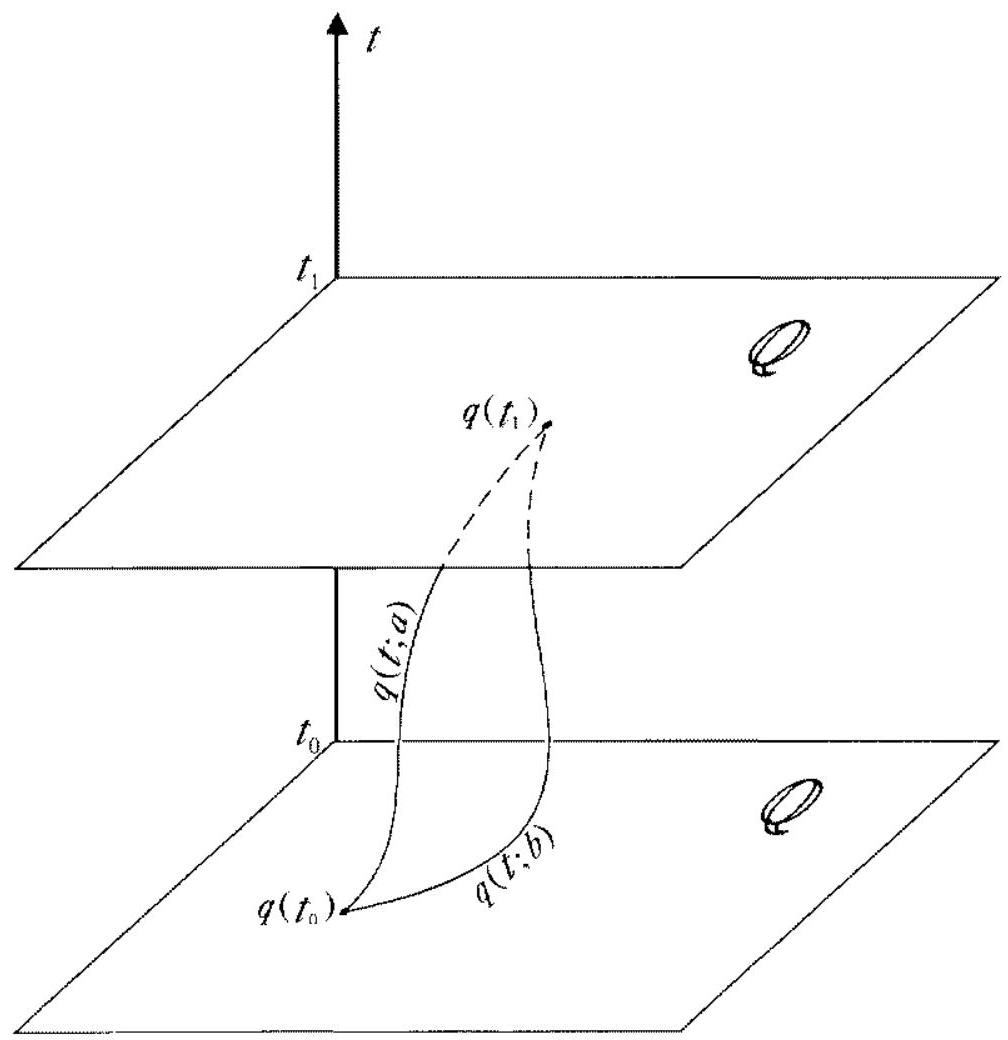
\includegraphics{variprin.jpg}
  \caption[]{Dos trayectorias posibles $ q(t ; a) $ y $ q(t ; b) $ desde $ q\left(t_{0}\right) $ hasta $ q\left(t_{1}\right) $. Los planos horizontales representan $ Q $ en los dos tiempos. Una familia continua de trayectorias posibles formaría una superficie en este diagrama, cuyas fronteras podrían ser $ q(t ; a) $ y $ q(t ; b) $.}
  \labfig{fig:}
\end{marginfigure}
\subsection{Ecuaciones de Euler-Lagrange}
Ahora procedemos a mostrar que la trayectoria física es la que da el valor mínimo de $ S $: minimizar $ S $ lleva a las ecuaciones de Lagrange. Consideremos una familia de muchas trayectorias $ q(t ; \epsilon) $, todas comenzando y terminando en $ q\left(t_{0}\right) $ y $ q\left(t_{1}\right) $, donde $ \epsilon $ es un índice que etiqueta cada trayectoria particular de la familia. Así como $ q(t ; a) $ y $ q(t ; b) $ conducen a diferentes acciones, cada $ q(t ; \epsilon) $ lleva a su correspondiente acción $ S(\epsilon) $. Entonces, el principio variacional establece que la trayectoria física es aquella para la cual la acción es un mínimo y que esto es independiente de la forma en que se elija la familia de trayectorias $ \epsilon $, siempre que contenga la física. Este es conocido como el principio variacional de Hamilton.

Más específicamente, requerimos que $ \epsilon $ tome sus valores de los números reales y parametrice la familia de trayectorias de forma continua y diferenciable. Esto significa que la familia forma una superficie conectada en el diagrama de la Fig. 3.1 y que la derivada parcial $ \partial q(t ; \epsilon) / \partial \epsilon $ existe para todos los valores de $ t $ en el intervalo $ \left[t_{0}, t_{1}\right] $. Todos los cálculos dependerán de $ \epsilon $ solo a través de derivadas, por lo que $ \epsilon $ puede cambiarse sin pérdida de generalidad agregando una constante arbitraria, y lo elegimos de manera que $ \epsilon=0 $ etiqueta la trayectoria que da el mínimo $ S $ en esa familia. (Por cierto, el requisito de diferenciabilidad se usará, y por lo tanto es necesario, solo en $ \epsilon=0 $.)

Las familias de trayectorias $ \epsilon $ se eligen de otra manera de manera bastante arbitraria, y solo por casualidad alguna de ellas contiene la trayectoria física. Sin embargo, en cualquier familia de este tipo, ya sea que incluya la trayectoria física o no, habrá una trayectoria para la cual $ S $ sea un mínimo. Esa trayectoria también puede incluirse en muchas otras familias $ \epsilon $, pero en general no dará el mínimo $ S $ en cada otra familia. Lo que el principio de Hamilton establece es que la trayectoria física da el mínimo $ S $ de cada familia en la que puede ser incluida. Matemáticamente, esto significa que para cualquier familia $ \epsilon $ tal, la trayectoria física satisface la ecuación

\begin{equation*}
\left.\frac{d S}{d \epsilon}\right|_{\epsilon=0} \equiv\left[\frac{d}{d \epsilon} \int_{t_{0}}^{t_{1}} L(q, \dot{q}, t) d t\right]_{\epsilon=0}=0 \tag{3.2}
\end{equation*}


A partir de ahora, abreviaremos $ d /\left.d \epsilon\right|_{\epsilon=0} $ como $ \delta $, por lo que (3.2) se convierte en

\begin{equation*}
\delta S \equiv \delta \int_{t_{0}}^{t_{1}} L(q, \dot{q}, t) d t=0 \tag{3.3}
\end{equation*}


Cabe recordar que en todas estas expresiones, todo se evalúa en $ \epsilon=0 $.

El siguiente paso es tomar la derivada de la integral con respecto a $ \epsilon $. La dependencia de $ \epsilon $ surge porque $ q $ y $ \dot{q} $ en el lagrangiano dependen de $ \epsilon $, así que

\begin{equation*}
\delta S=\int_{t_{0}}^{t_{1}} \delta L d t \tag{3.4}
\end{equation*}


Dado que $ \delta \equiv d /\left.d \epsilon\right|_{\epsilon=0} $,

\begin{equation*}
\delta L=\frac{\partial L}{\partial q^{\alpha}} \delta q^{\alpha}+\frac{\partial L}{\partial \dot{q}^{\alpha}} \delta \dot{q}^{\alpha} \tag{3.5}
\end{equation*}

Ahora, $ \dot{q}^{\alpha} \equiv \frac{d q^{\alpha}}{d t} $ es la velocidad generalizada a lo largo de una trayectoria especificada por un cierto valor de $ \epsilon $; es decir, la derivada temporal se toma para un $ \epsilon $ fijo. Esto debería escribirse como $ \frac{\partial q^{\alpha}}{\partial t} $, en lugar de $ \frac{d q^{\alpha}}{d t} $, pero en consonancia con la tradición y con la resolución final del problema, continuamos usando $ \frac{d q^{\alpha}}{d t} $. Dado que se trata de una derivada parcial, no hay problema en cambiar el orden de $ \frac{d}{d t} $ y $ \frac{\partial}{\partial \epsilon} $, y, por tanto, el orden de $ \frac{d}{d t} $ y $ \delta $. Así, tenemos

$$
\begin{aligned}
\frac{\partial L}{\partial \dot{q}^{\alpha}} \delta \dot{q}^{\alpha} & =\frac{\partial L}{\partial \dot{q}^{\alpha}} \frac{d}{d t} \delta q^{\alpha} \\
& =\frac{d}{d t}\left[\frac{\partial L}{\partial \dot{q}^{\alpha}} \delta q^{\alpha}\right]-\left[\frac{d}{d t} \frac{\partial L}{\partial \dot{q}^{\alpha}}\right] \delta q^{\alpha}
\end{aligned}
$$

Al insertar esto en la expresión para $ \delta L $, obtenemos


\begin{equation*}
\delta L=\left[\frac{\partial L}{\partial q^{\alpha}}-\frac{d}{d t} \frac{\partial L}{\partial \dot{q}^{\alpha}}\right] \delta q^{\alpha}+\frac{d}{d t}\left[\frac{\partial L}{\partial \dot{q}^{\alpha}} \delta q^{\alpha}\right] \tag{3.6}
\end{equation*}


Para un uso posterior, observamos que este resultado se obtuvo sin ninguna restricción sobre la variación de $ q(t, \epsilon) $ en los puntos finales.

Ahora, insertemos (3.6) en (3.4). Entonces,


\begin{equation*}
0=\delta S=\int_{t_{0}}^{t_{1}}\left[\frac{\partial L}{\partial q^{\alpha}}-\frac{d}{d t} \frac{\partial L}{\partial \dot{q}^{\alpha}}\right] \delta q^{\alpha} d t+\int_{t_{0}}^{t_{1}} \frac{d}{d t}\left[\frac{\partial L}{\partial \dot{q}^{\alpha}} \delta q^{\alpha}\right] d t \tag{3.7}
\end{equation*}


[Este resultado también podría haberse obtenido al insertar la Ec. (3.5) en la Ec. (3.4) e integrar el segundo término por partes.] El segundo integral aquí se obtiene fácilmente: es

$$
\left.\frac{\partial L}{\partial \dot{q}^{\alpha}} \delta q^{\alpha}\right|_{t_{1}}^{t_{1}}=0
$$

lo cual se anula porque en los puntos finales todas las trayectorias convergen, de modo que allí $ \delta q^{\alpha}=0 $. El término restante puede escribirse (ver Sección 2.2.2 para la definición de $ \Lambda_{\alpha} $):


\begin{equation*}
\int_{t_{0}}^{t_{1}} \Lambda_{\alpha} \delta q^{\alpha} d t=0 \tag{3.8}
\end{equation*}


Ahora, usemos el siguiente teorema (Gel'fand y Fomin, 1963). Sea $ f_{\alpha}, \alpha=1,2,\ldots,n $, un conjunto de $ n $ funciones integrables de una variable real $ t $ en un intervalo $ I $. Supongamos que


\begin{equation*}
\int_{I} f_{\alpha} h_{\alpha} d t=0 \tag{3.9}
\end{equation*}


para cualquier conjunto arbitrario de funciones integrables $ h_{\alpha} $ en el mismo intervalo, todas las cuales se anulan en sus puntos finales; entonces $ f_{\alpha}=0 $ para todos $ \alpha $. Dado que el principio de Hamilton se aplica a cualquier familia de trayectorias $ \epsilon $, los $ \delta q^{\alpha} $ son un conjunto de funciones arbitrarias de $ t $, al igual que los $ h_{\alpha} $, que se anulan en los puntos finales (recuerde que todo se evalúa en $ \epsilon=0 $). Por lo tanto, $ \Lambda_{\alpha}=0 $, o


\begin{equation*}
\frac{\partial L}{\partial q^{\alpha}}-\frac{d}{d t} \frac{\partial L}{\partial \dot{q}^{\alpha}}=0 \tag{3.10}
\end{equation*}


Estas son, por supuesto, las ecuaciones de Lagrange. Lo que nos dicen es que las funciones $ q^{\alpha}(t) $ que minimizan la acción, cuando se insertan junto con sus derivadas en la función lagrangiana y sus derivadas, son las mismas que satisfacen la ecuación de Lagrange.

En la Sección 3.2.2 será útil ver la Ec. (3.9) como un producto interno en un espacio vectorial $ \mathbb{F} $. Pensemos en los $ f_{\alpha} $ como los componentes de un vector $ f \in \mathbb{F} $ (y de manera similar $ h $), y escribamos

$$
\int_{I} f_{\alpha} h_{\alpha} d t \equiv(f, h)
$$

Entonces, el teorema citado arriba establece que si $ f $ es ortogonal a todos los vectores (arbitrarios $ h_{\alpha} $) en $ \mathbb{F} $, entonces $ f=0 $. Hay algunos puntos finos que podrían hacerse más rigurosos, pero esto será suficiente para nuestros propósitos. La derivación de las ecuaciones de Lagrange puede entonces expresarse en estos términos: la Ec. (3.8) establece que


\begin{equation*}
(\Lambda, \delta q)=0 \tag{3.11}
\end{equation*}


y dado que los $ \delta q $ son vectores arbitrarios y abarcan $ \mathbb{F} $, el vector $ \Lambda $ es ortogonal a todos los vectores en el espacio y, por lo tanto, se anula, que es el contenido de (3.10).
\subsection{Características de la acción}
garay

La acción de un sistema dinámico cuyas ecuaciones de movimiento son conocidas se construye de forma que estas se recuperen mediante el principio variacional. Sin embargo, la utilidad de este principio se debe a que, en muchos casos, es posible construir una acción para el sistema dinámico en cuestión mediante otras consideraciones (de simetría, por ejemplo), sin necesidad de conocer las ecuaciones de movimiento a priori.

He aquí algunas consideraciones ad hoc que se pueden tener en cuenta al construir la acción de un sistema dinámico:
\begin{itemize}
  \item La acción tiene dimensiones de momento angular.
  \item Consideraremos solo acciones locales en el tiempo. Por ejemplo, no consideraremos términos en la acción de la forma $\int \mathrm{d} t \mathrm{~d} t^{\prime} f\left(t, t^{\prime}\right) q(t) q\left(t^{\prime}\right)$.
  \todo{Esto es por la causalidad}
  \item Debe ser un funcional en el espacio de fases en velocidades $T \mathscr{Q}$. Podrían contener términos lineales en las segundas derivadas, pero mediante integración por partes, estos términos se pueden escribir como términos que dependen solo de primeras derivadas más términos que dependen de las condiciones iniciales y finales que no afectan a las ecuaciones de movimiento . Por ejemplo, la partícula libre se puede describir mediante la acción $S=\int \mathrm{d} t \delta_{i j} x^{i} \ddot{x}^{j}$, como es fácil comprobar . Esto es precisamente lo que ocurre cuando se añaden al lagrangiano derivadas totales $\dot{f}(q, \dot{q}, t)$ de funciones en el espacio de fases en velocidades ( $y$ no solo en el espacio de configuración), situación que no consideraremos aquí. Los sistemas con ecuaciones de evolución que contienen derivadas superiores tienen, salvo en situaciones concretas como la que acabamos de describir, comportamientos acausales.
  \item Si pretendemos describir sistemas con invariancias bajo ciertas transformaciones - simetrías-, es conveniente, pero no necesario, que la acción sea invariante bajo estas transformaciones. Por ejemplo, el segundo lagrangiano de la ecuación 1.2 describe la partícula libre, que es invariante bajo rotaciones, a pesar de que él mismo no lo sea.
  \item Para sistemas conservativos, la forma típica del lagrangiano es la diferencia entre la energía cinética y la potencial
  \begin{DispWithArrows}[format=c, displaystyle]
  L=T-V
  \end{DispWithArrows}
  , como se puede deducir a partir del principio de los trabajos virtuales y del principio de d'Alembert.
\end{itemize}

\subsection{Ligaduras}(114) (49-50) 

Las ligaduras aparecen en la dinámica cuando hay ciertas restricciones del movimiento. Miremos el siguiente ejemplo 
\begin{example}[Ejemplo ligaduras]
  Pensemos en una esfera que rueda sobre una superficie curva bajo la acción de la gravedad. La esfera está formada por muchas partículas cuyo movimiento está correlacionado, de modo que siempre forman una esfera rígida y siempre hay una de ellas en contacto con la superficie y, al rodar el cuerpo, instantáneamente en reposo. Las fuerzas que actúan sobre la esfera distan mucho de ser simples. Están compuestas por las fuerzas internas a la esfera (que la mantienen rígida), las fuerzas que le aplica la superficie sobre la que rueda (que la mantienen en contacto con dicha superficie y evitan que se deslice) y la fuerza de la gravedad. La fuerza de la gravedad se conoce a priori, pero las demás, las fuerzas de coacción, no. Lo que sí se sabe es que, bajo la acción de la gravedad y de las fuerzas de coacción, el cuerpo permanece sobre la superficie y sigue rodando. Podría parecer que para describir completamente el movimiento habría que encontrar las fuerzas de coacción, pero se demostrará lo contrario, que el movimiento puede obtenerse a partir de la fuerza gravitatoria y del conocimiento de las coacciones geométricas (es decir, de la forma de la superficie y del hecho de la rigidez); las fuerzas de coacción, si son necesarias, son más fáciles de encontrar después. Este ejemplo aparentemente sencillo de una esfera que rueda sobre una superficie curva es, en realidad, bastante complicado. La mayoría de las veces nos enfrentaremos a restricciones mucho más sencillas.
\end{example}

Hay dos tipos de ligaduras las cuales se definen de la siguiente manera:

\begin{definition}[Ligaduras Holonomas]
  Las ligaduras holónomas son aquellas que se pueden escribir mediante igualdades que involucran solo las variables de configuración y, quizá, el tiempo.
\end{definition}

\begin{definition}[Ligaduras Anholónomas]
  Las ligaduras anholónomas son aquellas que limitan el recorrido de las variables de configuración mediante desigualdades, que involucran las velocidades de forma que no se puedan transformar en otras que no las contengan o que, en general, no son holónomas.
\end{definition}



El método variacional de la Sección 3.1.1 seleccionó, entre todas las trayectorias que conectan $q\left(t_{0}\right)$ y $q\left(t_{1}\right)$, aquella que minimiza $S$. Sin embargo, este método debe ser modificado si el sistema está sujeto a restricciones, ya que las únicas trayectorias disponibles son aquellas que satisfacen las restricciones. Supongamos, por lo tanto, que el sistema está sujeto a $K<n$ restricciones independientes, en general no holonómicas (dependientes de la velocidad), de la forma

\begin{DispWithArrows}[displaystyle, format=c]
f_{I}(q, \dot{q} \cdot t)=0, \quad I=1,2, \ldots, K
\end{DispWithArrows}


Procedemos a aplicar el método variacional, ahora exigiendo que las trayectorias de comparación (las trayectorias entre las cuales se debe seleccionar la física) satisfagan las restricciones.

Comenzamos con la Ecuación (3.11), excepto que ahora $\delta q \in \mathbb{F}$, cuyos componentes son $\partial q^{\alpha} / \partial \epsilon$, no es arbitraria, ya que proviene de trayectorias $q(t ; \epsilon)$ que están restringidas por las Ecuaciones (3.12). La Ecuación (3.11) ahora dice que $\Lambda$ no es el vector nulo, sino que es ortogonal al subespacio $\mathbb{F}_{q} \subset \mathbb{F}$ generado por los $\delta q$ admisibles. Para encontrar las posibles $\Lambda$, debemos encontrar $\mathbb{F}_{q}$.

El subespacio $\mathbb{F}_{q}$ puede ser encontrado estableciendo con precisión cómo las Ecuaciones (3.12) restringen los vectores $\delta q$. Comencemos tomando las derivadas de las Ecuaciones (3.12) con respecto a $\epsilon$:

\begin{DispWithArrows}[displaystyle, format=c]
\frac{\partial f_{I}}{\partial \epsilon} \equiv \frac{\partial f_{I}}{\partial q^{\alpha}} \frac{\partial q^{\alpha}}{\partial \epsilon}+\frac{\partial f_{I}}{\partial \dot{q}^{\alpha}} \frac{\partial \dot{q}^{\alpha}}{\partial \epsilon}=0
\end{DispWithArrows}


Ahora multiplica cada una de estas ecuaciones por una función suficientemente bien comportada $\mu_{I}(t)$ y suma sobre $I$ (todas las sumas sobre $I$ están indicadas por signos de suma):

\begin{DispWithArrows}[displaystyle, format=c]
\int_{t_{0}}^{t_{1}} \sum_{l}\left[\mu_{l} \frac{\partial f_{l}}{\partial q^{\alpha}} \frac{\partial q^{\alpha}}{\partial \epsilon}+\mu_{l} \frac{\partial f_{l}}{\partial \dot{q}^{\alpha}} \frac{\partial \dot{q}^{\alpha}}{\partial \epsilon}\right] d t=0
\end{DispWithArrows}


Integra por partes, como en la derivación de la Ecuación (3.7), para obtener

\begin{DispWithArrows}[displaystyle, format=c]
\int_{t_{i}}^{l_{1}} \sum_{i}\left[\mu_{i} \frac{\partial f_{l}}{\partial q^{\alpha}}-\frac{d}{d t}\left(\mu_{1} \frac{\partial f_{l}}{\partial \dot{q}^{\alpha}}\right)\right] \frac{\partial q^{\alpha}}{\partial \epsilon} d t \equiv\left(\sum_{l} \chi_{l}, \delta q\right)=0
\end{DispWithArrows}

donde cada $\chi_{l}$ es el vector cuyas componentes son (sin suma sobre $I$)

\begin{DispWithArrows}[displaystyle, format=c]
\chi_{1 \alpha} \equiv \mu_{I} \frac{\partial f_{I}}{\partial q^{\alpha}}-\frac{d}{d t}\left(\mu_{I} \frac{\partial f_{I}}{\partial \dot{q}^{\alpha}}\right)
\end{DispWithArrows}


La Ecuación (3.14) da las restricciones sobre los vectores $\delta q$: son ortogonales a todos los posibles vectores $\chi_{I}$. El subespacio $\mathbb{F}_{4}$ que generan es ortogonal al subespacio $\mathbb{F}_{\chi} \subset \mathbb{F}$ generado por los $\chi_{1}$. (No hemos probado que ni $F_{4}$ ni $\mathbb{F}_{x}$ son subespacios, pero dejemos eso de lado).

Dado que $\Lambda$ es ortogonal a $\mathbb{F}_{q}$, que a su vez es ortogonal a $\mathbb{F}_{\chi}$, debe estar en $\mathbb{F}_{\chi}$. Es decir, existen constantes $\alpha_{1}$ tales que $\Lambda=\sum \alpha_{1} \chi_{1}$. Estos $\alpha_{1}$ pueden ser absorbidos en los $\mu_{1}$, escribiendo $\lambda_{I}(t)=\alpha_{I} \mu_{I}(t)$, y luego la definición de los $\Lambda_{\alpha}$ y la Ecuación (3.14) permiten que el resultado se exprese en la forma

\begin{DispWithArrows}[displaystyle, format=c]
\frac{d}{d t} \frac{\partial}{\partial \dot{q}^{\alpha}}\left(L+\sum \lambda_{l} f_{I}\right)-\frac{\partial}{\partial q^{\alpha}}\left(L+\sum \lambda_{l} f_{l}\right)=0
\end{DispWithArrows}

(los $\lambda_{1}$ se llaman multiplicadores de Lagrange). Este es el resultado de aplicar el principio variacional con restricciones: produce un conjunto de ecuaciones que se asemejan a las ecuaciones de EL para el Lagrangiano

\begin{DispWithArrows}[displaystyle, format=c]
\mathcal{L}=L+\sum \lambda_{1} f_{l}
\end{DispWithArrows}



Ahora tenemos las ecuaciones de Euler-Lagrange (EL) $n$ (3.15) y las ecuaciones de restricción $K$ (3.12) de las cuales debemos encontrar las funciones $q^{\alpha}(t)$ y $\lambda_{I}(t)$, que suman un total de $n+K$. Pero hay un problema serio: las Eqs. (3.15) son ecuaciones diferenciales de primer orden para los $\lambda_{I}$, y una solución requiere conocer los valores iniciales $\lambda_{l}\left(t_{0}\right)$. Este requisito es poco físico, ya que significa que deben conocerse las fuerzas iniciales de restricción (ver Problema 1) o, equivalente, las iniciales $\ddot{q}^{\alpha}$. Por esta razón, el enfoque variacional directo debe ser rechazado.

Sin embargo, si las restricciones son holonómicas (si los $f_{l}$ no dependen de los $\dot{q}^{\alpha}$), las Eqs. (3.15) se convierten en


\begin{DispWithArrows}[displaystyle, format=c]
\frac{d}{d t} \frac{\partial L}{\partial \dot{q}^{\alpha}}-\frac{\partial}{\partial q^{\alpha}}\left(L+\sum \lambda_{1} f_{I}\right)=0 \tag{3.17}
\end{DispWithArrows}


o


\begin{DispWithArrows}[displaystyle, format=c]
\frac{d}{d t} \frac{\partial L}{\partial \dot{q}^{\alpha}}-\frac{\partial L}{\partial q^{\alpha}}-\sum \lambda_{1} \frac{\partial f_{l}}{\partial q^{\alpha}}=0 \tag{3.18}
\end{DispWithArrows}


las cuales no involucran derivadas temporales de los $\lambda_{1}$. Así, la dificultad se evita. Para las restricciones holonómicas, las (3.17) son las ecuaciones aceptadas, y dado que los $f_{l}$ son independientes de $\dot{q}^{\alpha}$, las ecuaciones pueden escribirse como


\begin{DispWithArrows}[displaystyle, format=c]
\frac{d}{d t} \frac{\partial \mathcal{L}}{\partial \dot{q}^{\alpha}}-\frac{\partial \mathcal{L}}{\partial q^{\alpha}}=0 \tag{3.19}
\end{DispWithArrows}


con el $\mathcal{L}$ de (3.16).  
¿Qué se debe hacer en el caso general, cuando los $f_{1}$ dependen de los $\dot{q}^{\alpha}$? Una pista se obtiene al volver a las restricciones holonómicas, tomar sus derivadas temporales y llamar a estas las nuevas restricciones:


\begin{DispWithArrows}[displaystyle, format=c]
\hat{f}_{1} \equiv \frac{d f_{1}}{d t}=\frac{\partial f_{1}}{\partial q^{\alpha}} \dot{q}^{a}=0 \tag{3.20}
\end{DispWithArrows}


Las $\hat{f}_{1}(q, \dot{q}, t)$ son ahora restricciones dependientes de la velocidad, y en términos de ellas, la Eqs. (3.18) se convierte en


\begin{DispWithArrows}[displaystyle, format=c]
\frac{d}{d t} \frac{\partial L}{\partial \dot{q}^{\alpha}}-\frac{\partial L}{\partial q^{\alpha}}-\sum \lambda_{1} \frac{\partial \hat{f}_{I}}{\partial \dot{q}^{\alpha}}=0 \tag{3.21}
\end{DispWithArrows}


Este resultado es generalmente aceptado para restricciones dependientes de la velocidad, incluso si las $\hat{f}_{1}(q, \dot{q}, t)$, a diferencia de las de (3.20), son no lineales en los $\dot{q}^{\alpha}$.

\begin{marginfigure}[]
  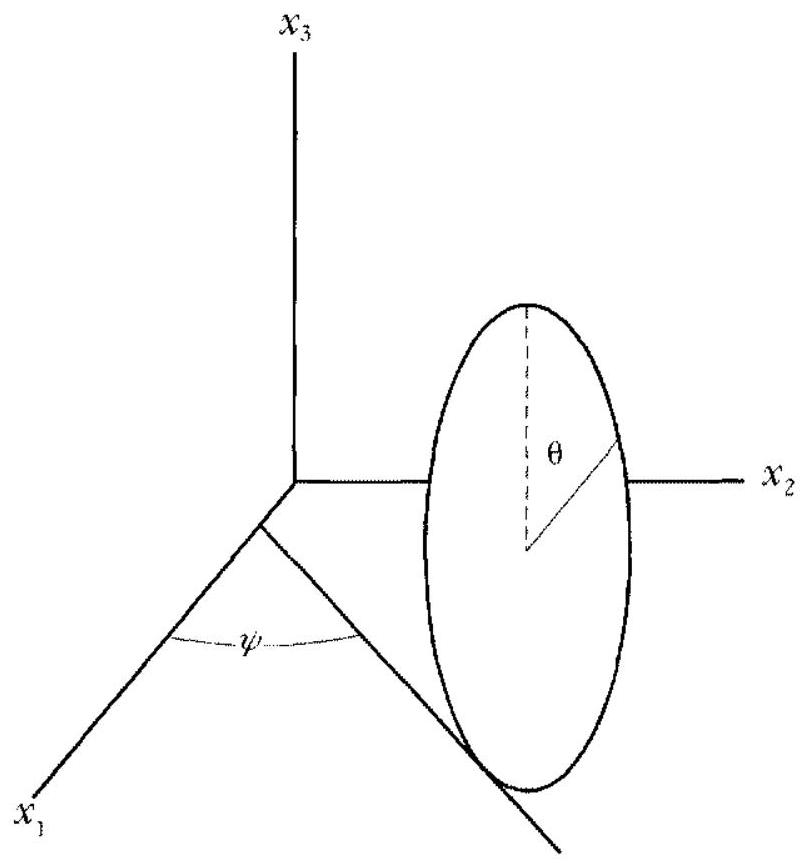
\includegraphics{exlig.jpg}
  \caption[]{Representación de las coordenadas generalizadas del ejemplo}
  \labfig{fig:exlig}
\end{marginfigure}

\begin{example}[Un disco de radio $R$ rueda sobre un plano horizontal perfectamente rugoso. (Esta es una restricción dependiente de la velocidad.) El disco está restringido a permanecer vertical. (Fig. 3.2) Escribe las ecuaciones de restricción y resuelve el movimiento en general.]
  


 La figura muestra las coordenadas generalizadas para este problema (las coordenadas del centro de masa del disco son $x_{1}$ y $x_{2}$). Las ecuaciones de restricción, que indican que el disco rueda, pueden escribirse como

$$
\begin{aligned}
& f_{1}=R \dot{\phi} \cos \psi-\dot{x}_{1}=0 \\
& f_{2}=R \dot{\phi} \sin \psi-\dot{x}_{2}=0
\end{aligned}
$$

El Lagrangiano es

$$
L=\frac{1}{2} I_{0} \dot{\phi}^{2}+\frac{1}{2} I_{1} \dot{\psi}^{2}+\frac{1}{2} m\left(\dot{x}_{1}^{2}+\dot{x}_{2}^{2}\right)
$$

donde $I_{0}$ es el momento de inercia del disco sobre su eje de simetría e $I_{1}$ es su momento de inercia sobre un diámetro. Las ecuaciones de movimiento son

$$
\Lambda_{\alpha}=\lambda_{I} \frac{\partial f_{I}}{\partial \dot{q}^{\alpha}}
$$

que, al desarrollarse, se convierten en

$$
\begin{align*}
& I_{0} \ddot{\phi}=\lambda_{1} R \cos \psi+\lambda_{2} R \sin \psi  \tag{3.22}\\
& I_{1} \ddot{\psi}=0  \tag{3.23}\\
& m \ddot{x}_{1}=-\lambda_{1}  \tag{3.24}\\
& m \ddot{x}_{2}=-\lambda_{2} \tag{3.25}
\end{align*}
$$

Las ecuaciones de restricción implican que $R \cos \psi=\dot{x}_{1} / \dot{\phi}$ y $R \sin \psi=\dot{x}_{2} / \dot{\phi}$, por lo que (3.22) se convierte en

$$
I_{0} \dot{\phi} \ddot{\phi}=\lambda_{1} \dot{x}_{1}+\lambda_{2} \dot{x}_{2}=-m\left(\dot{x}_{1} \ddot{x}_{1}+\dot{x}_{2} \ddot{x}_{2}\right)
$$

donde se han utilizado (3.24) y (3.25). Esto se integra inmediatamente para obtener

$$
I_{0} \dot{\phi}^{2}+m\left(\dot{x}_{1}^{2}+\dot{x}_{2}^{2}\right)=\text{constante}
$$

Pero las ecuaciones de restricción implican que $\dot{x}_{1}^{2}+\dot{x}_{2}^{2}=R^{2} \dot{\phi}^{2}$, por lo que $(I_{0}+m R^{2}) \dot{\phi}^{2}=\text{constante}$, o $\dot{\phi}=\text{constante}$. Así,

$$
\phi=\phi_{0}+\dot{\phi}_{0} t
$$

De (3.23) se sigue inmediatamente que

$$
\psi=\psi_{0}+\dot{\psi}_{0} t
$$

Insertando estos resultados en las ecuaciones de restricción e integrando se obtiene

$$
\begin{array}{ll}
\dot{x}_{1}=R \dot{\phi}_{0} \cos \left(\psi_{0}+\dot{\psi}_{0} t\right) ; & x_{1}=x_{10}+R \frac{\dot{\phi}_{0}}{\dot{\psi}_{0}} \sin \left(\psi_{0}+\dot{\psi}_{0} t\right) \\
\dot{x}_{2}=R \dot{\phi}_{0} \sin \left(\psi_{0}+\dot{\psi}_{0} t\right) ; & x_{2}=x_{20}-R \frac{\dot{\phi}_{0}}{\dot{\psi}_{0}} \cos \left(\psi_{0}+\dot{\psi}_{0} t\right)
\end{array}
$$

El disco rueda a una velocidad constante ($\dot{\phi}=\text{constante}$), cambiando de dirección también a una velocidad constante ($\dot{\psi}=\text{constante}$). Su centro de masa se mueve en un círculo de radio $\rho=\left|R \dot{\phi}_{0} / \dot{\psi}_{0}\right|$ centrado en $\left(x_{10}, x_{20}\right)$, para $\left(x_{1}-x_{10}\right)^{2}+\left(x_{2}-x_{20}\right)^{2}=\rho^{2}$. La velocidad del disco es constante, ya que $\dot{x}_{1}^{2}+\dot{x}_{2}^{2}=\left(R \dot{\phi}_{0}\right)^{2}=\text{constante}$.

Es evidente a partir de las Eqs. (3.24) y (3.25) que las $\lambda_{I}$ son las fuerzas que hacen que el disco se mueva de la manera en que lo hace. Estas son algunas de las fuerzas de restricción, ya que sin ellas el disco simplemente se movería en línea recta sobre el plano. Son solo algunas de las fuerzas de restricción porque hemos ignorado completamente las fuerzas que mantienen el disco vertical, tratando la masa como si estuviera toda concentrada en el punto de contacto sobre el plano y el disco como si no tuviera momento de inercia sobre el diámetro horizontal. Las componentes de las fuerzas de restricción en $x_{1}$ y $x_{}{2}$ son

$$
-\lambda_{1}=-R \dot{\phi}_{0} \dot{\psi}_{0} \sin \left(\psi_{0}+\dot{\psi}_{0} t\right), \quad-\lambda_{2}=R \dot{\phi}_{0} \dot{\psi}_{0} \cos \left(\psi_{0}+\dot{\psi}_{0} t\right)
$$

La fuerza de restricción es perpendicular a la velocidad (una fuerza centrífuga) y es proporcionada por la fricción con el plano. 

\end{example}


\section{Cantidades conservadas}(114-123)
\subsection{Coordenadas ciclicas}
A veces, las ecuaciones de Euler-Lagrange (EL) proporcionan una constante del movimiento de manera muy simple. Si una de las coordenadas generalizadas, digamos $q^{\beta}$, no aparece en el Lagrangiano (es una coordenada cíclica o ignorable), se cumple que $\partial L / \partial q^{\beta}=0$ y la ecuación EL de $\beta$ se expresa como


\begin{DispWithArrows}[displaystyle, format=c]
\frac{d}{d t} \frac{\partial L}{\partial \dot{q}^{\beta}}=0 
\end{DispWithArrows}


Esto implica claramente que $\partial L / \partial \dot{q}^{\beta}$ es una constante del movimiento. La función $p_{\beta}(q, \dot{q}, t)$ definida por


\begin{DispWithArrows}[displaystyle, format=c]
p_{\beta} \equiv \frac{\partial L}{\partial \dot{q}^{\beta}} 
\end{DispWithArrows}


se llama el momento generalizado conjugado a $q^{\beta}$. Si $q^{\beta}$ es ignorable\todo{Cuidad aquí que puede no aparecer en el Lagrangiano pero si en el extendido}, su momento conjugado $p_{\beta}$ proporciona un conjunto de subvariedades invariantes en $\mathbf{T Q}$. Es decir, si el punto de fase inicial se encuentra en alguna subvariedad cuya ecuación es de la forma $p_{\beta}=C$, el movimiento permanece en esa subvariedad.

Esto sugiere la utilidad de cambiar las coordenadas en $\mathbf{T} \mathbb{\sim}$ de $(q, \dot{q})$ a $(q, p)$. Más adelante, en la formulación hamiltoniana del Capítulo 5, haremos precisamente eso, pero implica pasar del haz tangente a otro conjunto llamado haz cotangente.

Supongamos, de manera más general, que alguna variable dinámica $\Gamma(q, \dot{q})$, que no necesariamente es uno de los $p_{\beta}$, se sabe que es constante en el movimiento. Su valor $C$ se determina por las condiciones iniciales $\Gamma\left(g_{0}, \dot{q}_{0}\right)=C$, y la ecuación $\Gamma(q, \dot{q})=C$ define una subvariedad invariantes de $(2 n-1)$ dimensiones (hiperficie) en $\mathbf{T Q}$. Cada $C$ diferente define una subvariedad invariante diferente, y las órbitas de fase yacen todas sobre tales subvariedades invariantes. Esto reduce el sistema dinámico de $2 n$ dimensiones en $\mathbf{T Q}$ a un conjunto de nuevos sistemas, cada uno de dimensión $2 n-1$ y cada uno etiquetado por su valor particular de $\Gamma$. De esta manera, cada constante del movimiento simplifica un sistema dinámico al reducir su dimensión en uno. Por esta razón, hay ventajas en encontrar sistemas de coordenadas con coordenadas ignorables: los momentos conjugados a los $q$ ignorables se conocen inmediatamente como constantes del movimiento.

Como ejemplo, nos dirigimos al Lagrangiano para el problema de fuerza central en el plano:


\begin{example}[Coordenadas cíclicas]


  \begin{DispWithArrows}[displaystyle, format=c]
    L=\frac{1}{2} \mu\left(\dot{r}^{2}+r^{2} \dot{\theta}^{2}\right)-V(r)
    \end{DispWithArrows}
    
    
    El ángulo $\theta$ es una coordenada ignorable, por lo que su momento conjugado, el momento angular $p_{\theta} \equiv \partial L / \partial \dot{\theta}$, se conserva. Cada una de sus subvariedades invariantes, dadas por
    
    
    \begin{DispWithArrows}[displaystyle, format=c]
    p_{\theta} \equiv \mu r^{2} \dot{\theta}=1
    \end{DispWithArrows}
    
    
    con diferentes valores $l$, define un nuevo sistema dinámico de un grado de libertad, como se discutió en la Sección 2.3.
\end{example}

Todo esto se puede expresar en términos de simetría, como se definió al comienzo de esta sección. Si $q^{\lambda}$ es ignorable, entonces $\partial L / \partial q^{\lambda}=0$, lo que significa que $L$ no cambia a medida que $q^{\lambda}$ varía, o $L$ es simétrico (o, como a menudo diremos, invariante) bajo la traducción en la dirección de $q^{\lambda}$ en $\mathbf{T Q}$.
\subsubsection{}
\subsection{Teorema de Noether}
\subsubsection{}
\subsubsection{}
\subsubsection{}

\section{Fuerzas disipativas}
(129-131)
\subsection{El oscilador harmónico amortiguado }


En previsión de los capítulos posteriores, nos dirigimos al ejemplo más conocido y sencillo de una fuerza proporcional a la velocidad, a saber, el oscilador armónico amortiguado. Comenzamos con un problema ligeramente más general para demostrar por qué el oscilador armónico surge con tanta frecuencia. Consideremos un sistema con un grado de libertad cuya Lagrangiana es
\begin{DispWithArrows}[displaystyle, format=c]
L=\frac{1}{2} \tau(q) \dot{q}^{2}-V(q) \tag{3.63}
\end{DispWithArrows}
donde $\tau$ es una función positiva definida (es decir, mayor que cero para todo $q$ ) y $V$ tiene un mínimo en algún valor $q_{0}$ de $q$. Para un pequeño desplazamiento $x$ desde $q_{0}$, el potencial $V$ se puede expandir en una serie de Taylor de la forma
$$
V(q)=V\left(q_{0}\right)+V^{\prime}\left(q_{0}\right) x+\frac{1}{2} V^{\prime \prime}\left(q_{0}\right) x^{2}+\frac{1}{6} V^{\prime \prime \prime}\left(q_{0}\right) x^{3}+\cdots
$$

Dado que $q_{0}$ es un mínimo para $V$, la primera derivada se anula. Toda función de energía potencial se define solo hasta una constante aditiva, la cual siempre se puede elegir para que $V\left(q_{0}\right)=0$; entonces la serie se convierte (cambiamos el argumento de $V$ de $q$ a $x$ )
\begin{DispWithArrows}[displaystyle, format=c]
V(x)=\frac{1}{2} k x^{2}+\frac{1}{6} s x^{3}+\cdots \tag{3.64}
\end{DispWithArrows}
donde $k \equiv V^{\prime \prime}\left(q_{0}\right)$ y $s \equiv V^{\prime \prime \prime}\left(q_{0}\right)$. Ahora expandimos también el término de energía cinética, nuevamente escribiendo todo en términos de $x$ (notar que $\dot{x}=\dot{q}$ ), para obtener
$$
\frac{1}{2} \tau(q) \dot{q}^{2}=\frac{1}{2} m \dot{x}^{2}+\frac{1}{2} r x \dot{x}^{2}+\cdots
$$
donde $m \equiv \tau\left(q_{0}\right)$ es positivo (bajo la suposición de que $\tau$ es una función positiva definida) y $r \equiv \tau^{\prime}\left(q_{0}\right)$. Entonces, si $k \neq 0$, para desplazamientos lo suficientemente pequeños desde el equilibrio, la Lagrangiana puede aproximarse por
\begin{DispWithArrows}[displaystyle, format=c]
L=\frac{1}{2} m \dot{x}^{2}-\frac{1}{2} k x^{2} \tag{3.65}
\end{DispWithArrows}
que es la Lagrangiana del oscilador armónico. En otras palabras, para vibraciones suficientemente pequeñas alrededor de un punto de equilibrio, todo sistema dinámico independiente del tiempo con un grado de libertad se comporta como un oscilador armónico, siempre que $V^{\prime \prime} \neq 0$ en el punto de equilibrio.

Si $V^{\prime \prime}\left(q_{0}\right)=0$ pero $V^{\prime \prime \prime}\left(q_{0}\right) \neq 0$, la fuerza es cuadrática en $x$ y, por lo tanto, siempre del mismo signo, siempre causando aceleraciones en la misma dirección. Entonces no es una fuerza restauradora y el equilibrio no es estable. De manera más general, para que ocurran oscilaciones, la potencia más baja en la expansión de Taylor del potencial debe ser par. Si $V^{\prime \prime \prime}\left(q_{0}\right)$ también se anula, el primer término en la expansión es cuártico y, aunque ocurren oscilaciones, el sistema es no lineal.

La Lagrangiana de la Ecuación (3.65) es la del oscilador armónico no amortiguado. Ahora añadimos una fuerza de amortiguación introduciendo la función de Rayleigh $\mathcal{F}=\hat{b} \dot{x}^{2}$. Entonces, de acuerdo con (3.60), la ecuación de movimiento es
\begin{DispWithArrows}[displaystyle, format=c]
m \ddot{x}+2 \hat{b} \dot{x}+k x=0 \tag{3.66}
\end{DispWithArrows}

Este es ahora el oscilador armónico amortiguado. Dos formas de su solución son
$$
\left.\begin{array}{l}
x(t)=e^{-\beta t}\left(A e^{t \omega t}+A^{*} e^{-t \omega t}\right)  \tag{3.67}\\
x(t)=e^{-\beta t}(a \cos \omega t+b \sin \omega t)
\end{array}\right\}
$$
donde $\beta=\hat{b} / m$ es el factor de amortiguación y $\omega=\sqrt{\omega_{0}^{2}-\beta^{2}}$, con $\omega_{0}=\sqrt{k / m}$. Las condiciones iniciales determinan las dos constantes reales de integración (ambas contenidas en la constante compleja $A$ en la primera forma y en $a$ y $b$ en la segunda).

Este sistema sigue siendo lineal, ya que $x$ y sus derivadas aparecen linealmente en la Ecuación (3.66). Si $V^{\prime \prime}\left(q_{0}\right)=0$ (como se mencionó anteriormente) o si la disipación no es proporcional a $\dot{x}$, es decir, si $\mathcal{F}$ no es cuadrática en $\dot{x}$, aparecerán algunas potencias superiores de $x$ y $\dot{x}$, lo que provocará que el sistema se vuelva no lineal. Los sistemas no lineales son considerablemente más complicados que los lineales. Serán discutidos con más detalle en el Capítulo 7.

El retrato de fase del oscilador no amortiguado (es decir, con $\beta=0$ ) se muestra en la Fig. 3.4. El retrato de fase consiste en elipses anidadas cuyas semiaxes son $c \equiv \sqrt{a^{2}+b^{2}}=|A|^{2}$ a lo largo del eje $x$ y $\omega c$ a lo largo del eje $\dot{x}$ (para el caso no amortiguado $\omega=\omega_{0}$ ). Cada elipse corresponde a un par de valores dados para $a$ y $b$, y la energía del movimiento está directamente relacionada con el área de la elipse (Problema 15).

Cuando $\beta \neq 0$, el retrato de fase consiste en curvas que convergen hacia el origen de $T \mathbb{Q}=\mathbb{R}^{2}$, como se muestra en la Fig. 3.5.

Si $\beta<\omega_{0}$, de modo que $\omega$ es real, las curvas son espirales, como la que se muestra en la Fig. 3.5(a), y el origen de $T \mathbb{Q}$ se llama el punto focal de la dinámica. El sistema oscila alrededor de $x=0$, con la amplitud disminuyendo en cada oscilación. Esto se llama el caso subamortiguado.

Si $\beta>\omega_{0}$, entonces $\omega \equiv i \nu$ es imaginaria y el sistema realiza como máximo una oscilación (dependiendo de las condiciones iniciales) antes de converger a $x=0$. Esto se llama el caso sobreamortiguado. Elige $v>0$ y observa que $\beta>v$. En términos de la constante real $v$,
$$
x(t)=e^{-\beta t}\left\{a e^{-\nu t}+b e^{v t}\right\}
$$


\section{Geometria}(134-136)

Una variedad diferenciable es, esencialmente, un conjunto de puntos que se puede describir por un atlas compuesto por mapas (a los que llamaremos cartas); una característica importante de un atlas es que las cartas que lo componen se deben superponer de forma suave. En este sentido, una variedad diferenciable es un conjunto de puntos que localmente se parece a $\mathbb{R}^{n}$.
\subsection{Campos vectoriales}

\begin{definition}[Vector tangente]
  Un vector tangente a una curva en un punto de una variedad diferenciable ( $y$, en particular, del espacio de fases) es un operador diferencial que asigna a cada función su derivada a lo largo de la curva. Más explícitamente, dada una curva $\gamma(s)$ parametrizada por $s$, definimos su vector tangente $\boldsymbol{X}$ como el operador que asigna a cada función $f$ el número
$$
X f=X(f):=\frac{\mathrm{d} f[\gamma(s)]}{\mathrm{d} s}=\frac{\mathrm{d} \gamma^{\alpha}}{\mathrm{d} s} \partial_{\alpha} f=\dot{\gamma}^{\alpha} \partial_{\alpha} f .
$$
\end{definition}

\begin{definition}[Campo vectorial]
  Un campo vectorial es una asignación suave de un vector a cada punto de la variedad. Los campos vectoriales son operadores diferenciales y, por tanto, son lineales y satisfacen la regla de Leibniz.
\end{definition}

Se define el conmutador de dos campos vectoriales $X$ y $Y$ como el campo vectorial
$$
[X, Y]=X Y-Y X=\left(X^{\alpha} \partial_{\alpha} Y^{\beta}-Y^{\alpha} \partial_{\alpha} X^{\beta}\right) \partial_{\beta}
$$
y satisface las siguientes propiedades:
\begin{itemize}
  \item linealidad, $\quad[a X+b Y, Z]=a[X, Z]+b[Y, Z] \quad \forall a, b \in \mathbb{R}$
  \item antisimetría, $[X, Y]=-[Y, X]$
  \item identidad de Jacobi, $\quad[X,[Y, Z]]+[Y,[Z, X]]+[Z,[X, Y]]=0$
\end{itemize}


Así, el conmutador dota al espacio tangente con la estructura de álgebra de Lie.
\subsection{Uno-formas}
\subsection{Ley de transformación I}
La ley de transformación de las componentes de un campo vectorial $X$ bajo un cambio arbitrario de coordenadas $\zeta^{\alpha} \rightarrow \zeta^{\prime \alpha}$ se deduce directamente de su definición:
$$
X^{\prime \alpha}=\frac{\partial \zeta^{\prime \alpha}}{\partial \zeta^{\beta}} X^{\beta}
$$
\subsection{Derivada de lie}
La derivada de Lie $\mathfrak{L}_{X}$ es un operador diferencial que da cuenta de cómo varían los campos tensoriales a lo largo de la curva generada por el campo vectorial $X$.

Dada una curva parametrizada por $s$ y cuyo vector tangente es $X$, podemos calcular cómo varía cualquier función a lo largo de la misma utilizando la definición de vector tangente: $\dot{f}=X f$. Por tanto,
$$
\dot{f}=\mathfrak{L}_{X} f=X f=X^{\alpha} \partial_{\alpha} f
$$

Notemos que, si la función $f$ tiene una dependencia explícita en el parámetro $s$, es necesario añadirla a esta expresión:
$$
\dot{f}=\mathfrak{L}_{X} f+\partial_{s} f=X f+\partial_{s} f
$$

La derivada de Lie de un campo vectorial $Y$ a lo largo de la curva generada por $X$ es un campo vectorial que tiene dos contribuciones, de acuerdo con la regla de Leibniz aplicada a la función $Y f$ para cualquier función $f$ :
$$
\mathfrak{L}_{X}(Y f)=\left(\mathfrak{L}_{X} Y\right) f+Y\left(\mathfrak{L}_{X} f\right)
$$

El primer miembro es la derivada de Lie de la función $Y^{\alpha} \partial_{\alpha} f$ y vale, por tanto, $X^{\beta} \partial_{\beta}\left(Y^{\alpha} \partial_{\alpha} f\right)$. Análogamente, el segundo término del segundo miembro se puede escribir de la forma $Y^{\beta} \partial_{\beta}\left(X^{\alpha} \partial_{\alpha} f\right)$. Concluimos así que
$$
\left(\mathfrak{L}_{X} Y\right) f=\left(X^{\beta} \partial_{\beta} Y^{\alpha}-Y^{\beta} \partial_{\beta} X^{\alpha}\right) \partial_{\alpha} f
$$
por lo que
$$
\mathfrak{L}_{X} Y=\left(X^{\beta} \partial_{\beta} Y^{\alpha}-Y^{\beta} \partial_{\beta} X^{\alpha}\right) \partial_{\alpha}=[X, Y]
$$

La primera contribución se debe a la manera en que cambian las componentes del campo $Y$ a lo largo de la curva. La segunda se debe a la propia evolución de los elementos de la base $\partial_{\alpha}$ a lo largo de la curva.

La derivada de Lie de una uno-forma $\boldsymbol{\sigma}$ es otra una uno-forma que se obtiene mediante el uso directo de la regla de Leibniz. La contracción $(\boldsymbol{\sigma}, Y)$ de $\boldsymbol{\sigma}$ con cualquier vector $Y$ involucra un producto tensorial y, además, es un escalar. Por tanto,
$$
\mathfrak{L}_{X}(\boldsymbol{\sigma}, Y)=\left(\boldsymbol{\sigma}, \mathfrak{L}_{X} Y\right)+\left(\mathfrak{L}_{X} \boldsymbol{\sigma}, Y\right)
$$

De esta expresión, obtenemos
$$
\mathfrak{L}_{X} \boldsymbol{\sigma}=\left(X^{\beta} \partial_{\beta} \sigma_{\alpha}+\sigma_{\beta} \partial_{\alpha} X^{\beta}\right) \mathrm{d} \zeta^{\alpha}
$$
\section{Variaciones temporales. Energía} (74)


\section{Partícula en un potencial}
Consideremos el lagrangiano de una partícula en un potencial
\begin{DispWithArrows}[displaystyle, format=c]
L=m \dot{\vec{x}}^{2} / 2-V(\vec{x}, t)
\end{DispWithArrows}
y estudiemos algunas posibles invariancias y sus cantidades conservadas correspondientes.
- Momento lineal. La acción es invariante bajo traslaciones infinitesimales constantes $\delta \vec{x}=\hat{n} \delta \epsilon$ en la dirección $\hat{n}$ o, en componentes, $\delta x^{i}=n^{i} \delta \epsilon$, si y solo si
\begin{DispWithArrows}[displaystyle, format=c]
\delta V=n^{i} \partial_{i} V \delta \epsilon=0
\end{DispWithArrows}
si y solo si $V$ no depende de la posición a lo largo de la dirección $\hat{n}$. En estas condiciones, el teorema de Noether nos garantiza que existe una cantidad conservada asociada:
\begin{DispWithArrows}[displaystyle, format=c]
\delta Q=p_{i} \delta x^{i}=n^{i} p_{i} \delta \epsilon
\end{DispWithArrows}
por tanto, el momento lineal $\hat{n} \cdot \vec{p}$ en la dirección $\hat{n}$ se conserva.
\begin{itemize}
  \item Momento angular. 
  
  La acción es invariante bajo rotaciones infinitesimales constantes $\delta \vec{x}=\hat{n} \times \vec{x} \delta \theta$ alrededor de una dirección $\hat{n}$ o, en coordenadas cartesianas, $\delta x^{i}=\epsilon^{i j k} n_{j} x_{k} \delta \theta$ si y solo si
  \begin{DispWithArrows}[displaystyle, format=c]
  \delta V=\epsilon^{i j k} n_{j} x_{k} \partial_{i} V \delta \theta=(\vec{x} \times \hat{n}) \cdot \vec{\nabla} V \delta \theta=0,
  \end{DispWithArrows}
  es decir, si y solo si $V$ es invariante bajo rotaciones alrededor de la dirección $\hat{n}$. En estas condiciones, el teorema de Noether nos garantiza que existe una cantidad conservada asociada:
  \begin{DispWithArrows}[displaystyle, format=c]
  \delta Q=p_{i} \delta x^{i}=p_{i} \epsilon^{i j k} n_{j} x_{k} \delta \theta=(\vec{x} \times \vec{p}) \cdot \hat{n} \delta \theta=\vec{L} \cdot \hat{n} \delta \theta ;
  \end{DispWithArrows}
  por tanto, el momento angular $\hat{n} \cdot \vec{L}$ en la dirección $\hat{n}$ se conserva.
  \item Energía. 
  
  La acción es invariante bajo traslaciones temporales infinitesimales constantes $\delta t=\delta \epsilon$ si y solo si
  \begin{DispWithArrows}[displaystyle, format=c]
  \delta V=\partial_{t} V \delta \epsilon=0
  \end{DispWithArrows}
  si y solo si $V$ es independiente del tiempo. En estas condiciones, el teorema de Noether nos garantiza que existe una cantidad conservada asociada:
  \begin{DispWithArrows}[displaystyle, format=c]
  \delta Q=\left[L-p_{i} \dot{x}^{i}\right] \delta t=-\left[m \dot{\vec{x}}^{2} / 2+V(\vec{x})\right] \delta \epsilon=-E \delta \epsilon
  \end{DispWithArrows}
  por tanto, la energía $E$ se conserva.
\end{itemize}
\section{Invariancia bajo reparametrizaciones temporales}
Supongamos que la acción de un sistema es invariante bajo reparametrizaciones temporales arbitrarias $t \rightarrow t^{\prime}=t+\delta t$ con $\delta t=\delta \epsilon(t)$. Entonces la cantidad conservada asociada es $\delta Q=-E \delta \epsilon(t)$. Puesto que $\delta \epsilon(t)$ es arbitrario y $\mathrm{d} \delta Q / \mathrm{d} t=0$, la única posibilidad es que la energía se anule. Esta es una característica general de los sistemas invariantes bajo reparametrizaciones temporales: la energía sobre trayectorias físicas se anula idénticamente.

Desde otro punto de vista, es interesante darse cuenta de que, bajo reparametrizaciones temporales, la acción de un sistema cambia en
\begin{DispWithArrows}[displaystyle, format=c]
\delta S=\int_{t_{1}}^{t_{2}} \mathrm{~d} t[(\delta \epsilon) L+\delta L]=\int_{t_{1}}^{t_{2}} \mathrm{~d} t\left[\left(L-\frac{\partial L}{\partial \dot{q}^{a}} \dot{q}^{a}\right)(\delta \epsilon)^{\cdot}+\frac{\partial L}{\partial t} \delta \epsilon\right] .
\end{DispWithArrows}

Para obtener esta expresión basta con tener en cuenta que, en este caso,
\begin{DispWithArrows}[displaystyle, format=c]
\delta L=\frac{\partial L}{\partial \dot{q}^{a}} \delta \dot{q}^{a}+\frac{\partial L}{\partial t} \delta t
\end{DispWithArrows}
hacer uso de la expresión 1.3 para $\delta \dot{q}$ y realizar algunas integraciones por partes . Por tanto, para que la acción sea invariante bajo reparametrizaciones temporales, es necesario y suficiente que el lagrangiano no dependa explícitamente del tiempo y que, además,
\begin{DispWithArrows}[displaystyle, format=c]
L-\frac{\partial L}{\partial \dot{q}^{a}} \dot{q}^{a}=0
\end{DispWithArrows}
condición necesaria y suficiente para que el lagrangiano sea homogéneo de grado 1 en $\dot{q}^{a}$. \todo{Esto es importante, ya que si tiene algún termino que sea $\propto \dot{q}^{a}\dot{q}^{b}$ (homogénea de grado 2 o superior), entonces la acción no será invariante }

Los sistemas invariantes bajo reparametrizaciones temporales son un ejemplo de una clase más general de sistemas lagrangianos con ligaduras, para los que no todas las ecuaciones de Euler-Lagrange son de segundo orden, es decir, son sistemas para los que $\operatorname{det}\left(\partial^{2} L / \partial \dot{q}^{a} \partial \dot{q}^{b}\right)=0$. Para verlo en este caso particular, basta con calcular la derivada con respecto a $\dot{q}^{b}$ de la expresión anterior y notar que las velocidades $\dot{q}^{a}$ son independientes.

Finalmente, notemos que, si elegimos un parámetro temporal específico que rompa la invariancia bajo reparametrizaciones, la energía ya no será nula y dependerá del parámetro elegido: el concepto de energía depende del parámetro temporal de evolución elegido, es decir, ;depende del reloj que utilicemos!
\begin{example}
  La acción
\begin{DispWithArrows}[displaystyle, format=c]
S=\pi_{0} \int \mathrm{~d} \sigma \sqrt{\frac{\dot{\vec{x}}^{2}}{}}
\end{DispWithArrows}
donde $\pi_{0}$ es una constante con dimensiones de momento lineal, $\sigma$ es un parámetro temporal arbitrario y $\stackrel{\rightharpoonup}{x}:=\mathrm{d} \vec{x} / \mathrm{d} \sigma$, es invariante bajo reparametrizaciones temporales, como se puede comprobar directamente o mediante el grado de homogeneidad del lagrangiano. Las ecuaciones de movimiento son 
\begin{DispWithArrows}[displaystyle, format=c]
\frac{\stackrel{\circ}{\vec{x}}}{\sqrt{\frac{\dot{x}^{2}}{2}}}=\hat{n}
\end{DispWithArrows}
donde $\hat{n}$ es un vector unitario constante. Vemos que esta partícula mantiene siempre un movimiento rectilíneo, pero el módulo de su velocidad no está determinado y, de hecho, es una función arbitraria del tiempo. Esta acción describe el movimiento de una partícula libre en términos de un tiempo arbitrario, no del tiempo absoluto empleado para definir los sistemas de referencia galileanos. La energía de esta partícula con respecto a este parámetro temporal arbitrario $\sigma$ es
\begin{DispWithArrows}[displaystyle, format=c]
E^{(\sigma)}=\frac{\stackrel{\circ}{x}}{\sqrt{\dot{\vec{x}}^2}} \cdot \frac{L}{\pi_0} .
\end{DispWithArrows}
\end{example}

\section{Simetrías gauge}
La invariancia bajo reparametrizaciones temporales es un ejemplo de simetría gauge. Las simetrías gauge permiten utilizar distintas descripciones matemáticas de la misma situación física (por ejemplo, distintas parametrizaciones temporales).

Las simetrías gauge se caracterizan porque desproveen parcialmente de significado físico a las variables de configuración: si la trayectoria $q(t)$ es una solución de las ecuaciones de Euler-Lagrange con unas ciertas condiciones iniciales $q(0)$ y $\dot{q}(0)$, entonces también lo será $q(t)+\delta q(t)$ con las mismas condiciones iniciales. Por ejemplo, en un sistema cuyo lagrangiano es invariante bajo reparametrizaciones temporales, si $q(t)$ es una solución con ciertas condiciones iniciales, también lo será cualquier trayectoria $q(t+\delta \epsilon(t))$ con las mismas condiciones iniciales. Así, tendremos clases de equivalencia de soluciones (relacionadas mediante transformaciones gauge) como trayectorias físicas.

Además, las cantidades Noether asociadas a las simetrías gauge son siempre nulas, lo que implica que tenemos ligaduras, es decir, que no todas las ecuaciones de Euler-Lagrange son de segundo orden, como hemos visto para el caso particular de la invariancia bajo reparametrizaciones. En efecto, en general, si tenemos una simetría gauge, entonces 
\begin{DispWithArrows}[displaystyle, format=c]
\delta Q=0.
\end{DispWithArrows}

Si derivamos esta expresión con respecto a $\dot{q}^{b}$, obtenemos la ecuación 
\begin{DispWithArrows}[displaystyle, format=c]
\frac{\partial^{2} L}{\partial \dot{q}^{a} \partial \dot{q}^{b}}\left(\delta q^{a}-\dot{q}^{a} \delta t\right)=0.
\end{DispWithArrows}

Puesto que las variaciones son obviamente independientes, podemos concluir que 
\begin{DispWithArrows}[displaystyle, format=c]
\operatorname{det}\left(\partial^{2} L / \partial \dot{q}^{a} \partial \dot{q}^{b}\right)=0.
\end{DispWithArrows}

Es importante notar la diferencia con las simetrías físicas, para las que las cantidades Noether conservadas no se anulan idénticamente. En este caso, la transformación caracterizada por $\delta q$, transforma una solución con unas condiciones iniciales $q(0)$ y $\dot{q}(0)$ en otra con otras condiciones iniciales $q(0)+\delta q(0)$ y $\dot{q}(0)+\delta \dot{q}(0)$. Por ejemplo, la invariancia bajo traslaciones $\delta q=\delta \epsilon$ relaciona una solución con condiciones iniciales $q(0)$ y $\dot{q}(0)$ en otra con condiciones iniciales $q(0)+\delta \epsilon$ y $\dot{q}(0)$; la invariancia bajo traslaciones temporales constantes $\delta t=\delta \epsilon$, la convierte en la solución con condiciones iniciales $q(\delta \epsilon)$ y $\dot{q}(\delta \epsilon)$.


\section{Dinámica Relativista}

Antes de empezar con la dinámica relativista y como parece que cuarto solo se da relatividad y calculo tensorial, es recomendable mirarse el apéndice de relatividad. 

\subsection{Accion}
Consideremos un conjunto de partículas relativistas descritas por sus posiciones espaciotemporales $x_{n}^{\mu}$ y sus correspondientes velocidades $\dot{x}_{n}^{\mu}$, donde el punto representa la derivada con respecto a su tiempo propio, y veamos cuál puede ser una posible acción para este sistema.

Si tuviésemos una sola partícula, una posible acción podría ser de la forma $S=\int \mathrm{d} \tau L\left(x^{\mu}, \dot{x}^{\mu}, \tau\right)$, donde $\tau$ es el tiempo propio de la partícula. Sin embargo, el cuadrado de la cuadrivelocidad tiene un valor fijo, $\dot{x}^{2}=-c^{2}$, es decir, el problema variacional correspondiente tiene una ligadura anholónoma que debemos introducir mediante un multiplicador de Lagrange siguiendo el procedimiento descrito en $\$ 1.1 .6$. Aún así, el tratamiento inadecuado de ignorar la ligadura y de proceder como si el sistema fuese libre proporciona el resultado correcto para una partícula libre o en interacción con un campo electromagnético.

Con más de una partícula, nos encontramos con la dificultad adicional de decidir para qué sistema $\tau$ es el tiempo propio. No parece razonable (aunque posible) elegir una partícula como privilegiada y plantear la evolución con respecto al tiempo propio de esa partícula concreta. Esto nos lleva a considerar acciones que no dependan del parámetro temporal que utilicemos, es decir, a considerar acciones invariantes bajo reparametrizaciones. Además, esta es una simetría que poseen las ecuaciones de movimiento.

En la construcción de una acción relativista, nos guiaremos por los siguientes criterios:

\begin{itemize}
  \item  Debe ser invariante bajo reparametrizaciones temporales.
\item  Debe ser invariante bajo transformaciones de Lorentz, para que sea independiente del sistema de referencia inercial escogido.
\item  En el límite no relativista y en ausencia de interacciones, debemos recuperar el lagrangiano $\sum_{n} m_{n} \vec{v}_{n}^{2} / 2$.
\end{itemize}

\subsubsection{Partículas libres}
Comencemos por definir la acción de un conjunto de partículas libres relativistas. La invariancia bajo reparametrizaciones temporales fuerza que el lagrangiano sea homogéneo en las velocidades y la invariancia Lorentz a que dependa de las velocidades a través de su cuadrado. Por tanto, el término de la acción correspondiente a la partícula $n$-ésima debe ser proporcional a 
\begin{DispWithArrows}[displaystyle, format=c]
\int \mathrm{d} \sigma \sqrt{-\grave{x}_{n}^{2}},
\end{DispWithArrows}
donde $\sigma$ es un parámetro temporal arbitrario y $\dot{x}=\mathrm{d} x / \mathrm{d} \sigma$. Este factor tiene dimensiones de longitud. Para que tenga dimensiones de acción, multiplicamos por $-m_{n} c$ donde $m_{n}$ es la masa de la $n$-ésima partícula. La razón para incluir el signo negativo será discutida en breve. Entonces podemos escribir la acción de un sistema de partículas libres como
\begin{DispWithArrows}[displaystyle, format=c]
S=\int \mathrm{d} \sigma\left[-\sum_{n} m_{n} c \sqrt{-\dot{x}_{n}^{2}}\right].
\end{DispWithArrows}

Puesto que $\dot{x}_{n}$ no es la cuadrivelocidad, no está sujeta a ninguna ligadura y puede ser variada libremente. En efecto, es fácil comprobar que $\grave{x}_{n}^{2}=-\left[c /\left(\mathrm{d} \sigma / \mathrm{d} \tau_{n}\right)\right]^{2}$ es libre ya que $\mathrm{d} \sigma / \mathrm{d} \tau_{n}$ es arbitraria, donde $\tau_{n}$ es el tiempo propio de la partícula $n$-ésima.

También podemos escribir esta acción, ya deparametrizada, en términos del tiempo $t$ correspondiente a un cierto sistema de referencia inercial. Para ello, elegimos como tiempo $\sigma$ el parámetro temporal $t$. En el instante $t$, las partículas se hallarán en la posición espaciotemporal $x_{n}^{\mu}=\left(c t, x_{n}^{i}\right)$ con respecto al sistema de referencia inercial elegido, por lo que
\begin{DispWithArrows}[displaystyle, format=c]
\dot{x}_{n}^{\mu}=\mathrm{d} x_{n}^{\mu} / \mathrm{d} t=\left(c, v_{n}^{i}\right), \quad \sqrt{-\dot{x}_{n}^{2}}=c \sqrt{1-\vec{v}_{n}^{2} / c^{2}}.
\end{DispWithArrows}

Por tanto, la acción también se puede escribir de la forma
\begin{DispWithArrows}[displaystyle, format=c]
S=-\sum_{n} m_{n} c^{2} \int \mathrm{~d} t \sqrt{1-\vec{v}_{n}^{2} / c^{2}}.
\end{DispWithArrows}

En el límite no relativista, podemos expandir esta acción en serie de potencias de la velocidad tridimensional de la $n$-ésima partícula $v_{n} / c$ :
\begin{DispWithArrows}[displaystyle, format=c]
\begin{aligned}
S & =-\sum_{n} m_{n} c^{2} \int \mathrm{~d} t\left[1-\frac{1}{2} \frac{\vec{v}_{n}^{2}}{c^{2}}+\mathscr{O}\left[\left(v_{n} / c\right)^{4}\right]\right] = \\
& =-\sum_{n} m_{n} c^{2} \int \mathrm{~d} t+\int \mathrm{d} t\left[\sum_{n} \frac{1}{2} m_{n} \vec{v}_{n}^{2}\right]+\mathscr{O}\left[\left(v_{n} / c\right)^{4}\right].
\end{aligned}
\end{DispWithArrows}

El primer término es constante (corresponde a una derivada total en el lagrangiano) y el segundo es la acción de un sistema de partículas libres no relativistas. Notemos que, si no hubiésemos introducido el signo negativo en $-m_{n} c$, habríamos obtenido la acción no relativista tradicional cambiada de signo.
\subsubsection{Partículas en un campo electromagenético}
Los campos electromagnéticos $\vec{E}$ y $\vec{B}$ están descritos por los potenciales escalar $\phi$ y vector $\vec{A}$, de forma que
$$
\vec{B}=\vec{\nabla} \times \vec{A}, \quad \vec{E}=-\vec{\nabla} \phi-\partial_{t} \vec{A} .
$$

Estos potenciales se pueden ver como las componentes temporal y espacial de un cuadrivector ${ }^{4} A^{\mu}=\left(\phi / c, A^{i}\right)$, en términos del cual, el campo electromagnético adquiere la forma

\begin{equation}
F_{\mu \nu}=\partial_{\mu} A_{\nu}-\partial_{\nu} A_{\mu} \tag{1.5}
\end{equation}


Obviamente, $F_{\mu \nu}$ es un tensor antisimétrico cuyas componentes son 
$$
F_{0 i}=-F_{i 0}=-E_{i} / c, \quad F_{i j}=\epsilon_{i j k} B^{k} .
$$

A la vista de la expresión 1.5 del campo electromagnético, dos potenciales $A_{\mu}$ y $A_{\mu}^{\prime}$ que se diferencien en $\partial_{\mu} f$, donde $f(x)$ es una función arbitraria de la posición espaciotemporal, determinan el mismo campo electromagnético .

La acción de un sistema de partículas en un campo electromagnético ha de ser, como ya hemos apuntado, invariante bajo reparametrizaciones temporales, invariante Lorentz y debe tener el límite no relativista adecuado. Además, como en el lagrangiano debe aparecer el potencial vector, la acción debe ser invariante bajo transformaciones gange $A_{\mu} \rightarrow A_{\mu}+\partial_{\mu} f$. Notemos que, en este tema, $A_{\mu}$ es un campo externo; por tanto, esta transformación gauge no es como las discutidas en $\$ 1.2 .6$, que involucran transformaciones de las variables dinámicas. Sí lo será en el tema 5 , cuando $A_{\mu}$ sea un campo dinámico cuya evolución debamos estudiar. Notemos por último que cada partícula interacciona con el campo electromagnético independientemente, es decir, que la acción será la suma de las acciones correspondientes a cada partícula, lo que nos permite estudiar cada partícula por separado.

Los únicos cuadrivectores de los que disponemos para construir la acción son $\grave{x}^{\mu} \mathrm{d} \sigma$ y $A^{\mu}$. Además, disponemos también del tensor métrico $\eta_{\mu \nu}$ y del psuedotensor de Levi-Civita $\varepsilon^{\mu \nu \rho \sigma}$. Los únicos invariantes Lorentz independientes que podemos construir con estos elementos son $A^{2}, \mathrm{~d} \sigma \dot{x}^{\mu} A_{\mu}$ y $\dot{x}^{2}(\mathrm{~d} \sigma)^{2}$. Así, el término más general invariante Lorentz e invariante bajo reparametrizaciones

\footnotetext{
${ }^{4}$ En este curso, no demostraremos esta afirmación.
}
deberá estar construido con estos elementos y deberá ser, además, homogéneo en las velocidades (para asegurar la invariancia bajo reparametrizaciones). Su forma más general es 
$$
\int \mathrm{d} \sigma \sqrt{-\dot{x}^{2}} H\left(A^{2}, \dot{x}^{\mu} A_{\mu} / \sqrt{-\dot{x}^{2}}\right)
$$
donde $H(x, y)$ es una función arbitraria. La invariancia de la acción bajo transformaciones gauge del campo electromagnético elimina todos los posibles términos salvo dos: $\int \mathrm{d} \sigma \sqrt{-\dot{x}^{2}}$ y $\int \mathrm{d} \sigma \dot{x}^{\mu} A_{\mu}$, correspondientes a $H(x, y)=1$ por un lado, y a $H(x, y)=y$ por el el otro .

Así, la acción de un sistema de partículas sometidas a un campo electromagnético externo será

\begin{equation}
S=\int \mathrm{d} \sigma L^{(\sigma)}=\sum_{n} \int \mathrm{~d} \sigma\left[-m_{n} c \sqrt{-\dot{x}_{n}^{2}}+q_{n} \dot{x}_{n}^{\mu} A_{\mu}\left(x_{n}\right)\right] 
\end{equation}

donde $q_{n}$ es la carga de la $n$-ésima partícula. Cuando sea necesario, como ocurre con el lagrangiano, especificaremos con el superíndice ${ }^{(\sigma)}$ la dependencia de la parametrización. Es fácil ver que esta acción tiene el límite no relativista correcto.
\subsection{Ecuaciones del movimiento}
Las ecuaciones del Euler-Lagrange correspondientes a la acción 1.6 de un sistema de partículas en un campo electromagnético son 
$$
\begin{aligned}
0=\frac{\delta S}{\delta x_{n}^{\mu}} & =\frac{\partial L^{(\sigma)}}{\partial x_{n}^{\mu}}-\frac{\mathrm{d}}{\mathrm{~d} \sigma} \frac{\partial L^{(\sigma)}}{\partial \dot{x}_{n}^{\mu}}= \\
& =-m_{n} c \frac{\mathrm{~d}}{\mathrm{~d} \sigma} \frac{\dot{x}_{n \mu}}{\sqrt{-\dot{x}_{n}^{2}}}+q_{n} \dot{x}_{n}^{\nu} F_{\mu \nu}\left(x_{n}\right) .
\end{aligned}
$$

Puesto que las partículas no interaccionan entre sí, podemos estudiar la evolución de cada una por separado en términos de su tiempo propio. La ecuación de evolución para cada una de ellas es entonces
$$
m_{n} \ddot{x}_{n \mu}=q_{n} \dot{x}_{n}^{\nu} F_{\mu \nu}\left(x_{n}\right) .
$$

Escogiendo $\sigma$ como el tiempo $t$ en un sistema de referencia inercial cualquiera, las componentes espacial y temporal de estas ecuaciones adquieren la forma 
$$
\frac{\mathrm{d}}{\mathrm{~d} t}\left(m_{n} \gamma_{n} \vec{v}_{n}\right)=q_{n}\left(\vec{E}+\vec{v}_{n} \times \vec{B}\right), \quad \frac{\mathrm{d}}{\mathrm{~d} t}\left(m_{n} \gamma_{n} c^{2}\right)=q_{n} \vec{v}_{n} \cdot \vec{E}
$$

La primera ecuación nos dice que la derivada temporal del momento cinético $m_{n} \gamma_{n} \vec{v}_{n}$ es igual a la fuerza de Lorentz. La segunda ecuación nos dice que el campo eléctrico realiza un trabajo empleado en cambiar la energía cinética $m_{n} \gamma_{n} c^{2}$ de cada partícula y que el campo magnético no realiza trabajo. Además, esta ecuación se puede reescribir de la forma 
$$
\frac{\mathrm{d}}{\mathrm{~d} t}\left(m_{n} \gamma_{n} c^{2}+q_{n} \phi\right)=q_{n}\left(\partial_{t} \phi-\vec{v}_{n} \cdot \partial_{t} \vec{A}\right)
$$

Por tanto, si el potencial vector $A^{\mu}=(\phi / c, \vec{A})$ es independiente del tiempo $x^{0}=c t$, entonces se conserva la energía de cada partícula $E_{n}=m_{n} \gamma_{n} c^{2}+q_{n} \phi\left(\vec{x}_{n}\right)$ correspondiente a este tiempo coordenado.
$\diamond$ EJERCICIO: Encontrar el límite no relativista de todos los resultados de esta sección.
\subsection{Cantidades Conservadas}
El teorema de Noether nos garantiza que, si la acción es invariante bajo una cierta transformación infinitesimal $\left(\delta x_{n}^{\mu}, \delta \sigma\right)$ que puede afectar tanto a las variables de configuración como al parámetro temporal, entonces existe una cantidad conservada dada por
$$
\delta Q=\sum_{n}\left[p_{n \mu} \delta x_{n}^{\mu}-E_{n}^{(\sigma)} \delta \sigma\right]
$$
donde
$$
p_{n \mu}=\partial L^{(\sigma)} / \partial \grave{x}_{n}^{\mu}, \quad E_{n}^{(\sigma)}=p_{n \mu} \dot{x}_{n}^{\mu}-L^{(\sigma)}
$$

Notemos que, por construcción, el cuadrimomento no depende de la parametrización. Para un sistema de partículas acopladas a un campo electromagnético,
$$
p_{n \mu}=m_{n} \frac{\dot{x}_{n \mu}}{\sqrt{-\dot{x}_{n}^{2}}}+q_{n} A_{n \mu}=m_{n} \dot{x}_{n \mu}+q_{n} A_{n \mu}
$$

Por otro lado, es fácil comprobar que la energía $E^{(\sigma)}$ asociada al tiempo arbitrario $\sigma$ de este sistema se anula, como debe ocurrir puesto que la acción 1.6 es invariante bajo reparametrizaciones temporales.
\subsubsection{Cuadrimomento}
Cuando la acción es invariante bajo traslaciones infinitesimales constantes (activas) en una dirección espaciotemporal $n^{\mu}$ que no afectan al parámetro temporal $\delta x_{n}^{\mu}=n^{\mu} \delta \epsilon$, la cantidad Noether conservada es la proyección del cuadrimomento conjugado total en esa dirección
$$
n^{\mu} P_{\mu}=n^{\mu} \sum_{n} p_{n \mu}
$$

Es importante notar que la cantidad que se conserva no es el momento cinético total $\sum_{n} m_{n} \dot{x}_{n}^{\mu}$ sino el cuadrimomento conjugado total. Para sistemas cuyo lagrangiano no tiene dependencia lineal en las velocidades, ambos obviamente coinciden.

Si $n^{\mu}$ es un vector espacial, existe un sistema de referencia inercial en el que $n^{0}=0$ y la cantidad conservada es obviamente el momento lineal (relativista) $\hat{n} \cdot \vec{P}$ en esa dirección y en ese sistema de referencia. Por ejemplo, para un sistema de partículas cargadas,
$$
\hat{n} \cdot \vec{P}=\hat{n} \cdot \sum_{n} \vec{p}_{n}, \quad \vec{p}_{n}=\gamma_{n} m_{n} \vec{v}_{n}+q_{n} \vec{A}\left(x_{n}\right)
$$

Si $n^{\mu}$ es un vector temporal, entonces existe un sistema de referencia inercial en el que $n^{\mu}=(1,0,0,0)$; la cantidad conservada correspondiente es la energía correspondiente a traslaciones temporales en ese sistema de referencia inercial
$$
c P^{0}=\sum_{n}\left[\gamma_{n} m_{n} c^{2}+q_{n} \phi\left(x_{n}\right)\right]
$$

Para que la acción 1.6, sea invariante bajo traslaciones en la dirección $n^{\mu}$, basta con que el potencial vector $A_{\mu}$ sea independiente de la posición en esa dirección, es decir, que $n^{\mu} \partial_{\mu} A_{\nu}=0$.
\subsubsection{Cuadrimomento angular}
Toda transformación de Lorentz se puede escribir como una composición de transformaciones de Lorentz infinitesimales $\Lambda^{\mu}{ }_{\nu}=\delta_{\nu}{ }^{\mu}+\delta \omega^{\mu}{ }_{\nu}$ (ver apéndice C). Una transformación de Lorentz infinitesimal (activa) de las posiciones adquiere la forma:
$$
\delta x_{n}^{\mu}=-\delta \omega^{\mu}{ }_{\nu} x_{n}^{\nu} .
$$

Si la acción es invariante bajo alguna de las transformaciones de Lorentz (de parámetros $\delta \omega^{\mu}{ }_{\nu}$ ), entonces existe una cantidad conservada asociada
$$
\begin{aligned}
\delta Q & =\sum_{n} p_{n \mu} \delta x_{n}^{\mu}=-\sum_{n} p_{n}^{\mu} x_{n}^{\nu} \delta \omega_{\mu \nu}= \\
& =\frac{1}{2} \sum_{n} l_{n}^{\mu \nu} \delta \omega_{\mu \nu}=\frac{1}{2} J^{\mu \nu} \delta \omega_{\mu \nu}
\end{aligned}
$$
donde $l_{n}^{\mu \nu}=x_{n}^{\mu} p_{n}^{\nu}-x_{n}^{\nu} p_{n}^{\mu}$ es el momento angular cuadridimensional de la partícula $n$-ésima y $J^{\mu \nu}=\sum_{n} l_{n}^{\mu \nu}$ es el cuadrimomento angular total.

Si separamos los boosts de las rotaciones espaciales, podemos reescribir esta expresión de la forma (ver apéndice C )
$$
\delta Q=\delta \vec{\theta} \cdot \vec{J}+\delta \vec{\zeta} \cdot \vec{K}
$$
donde
$$
\begin{aligned}
J^{i} & =\frac{1}{2} \epsilon^{i j k} J_{j k}, & \delta \theta^{i} & =\frac{1}{2} \epsilon^{i j k} \delta \omega_{j k}, \\
K_{i} & =J_{i 0}, & \delta \zeta_{i} & =\delta \omega_{0 i} .
\end{aligned}
$$

En particular, si la acción es invariante bajo rotaciones alrededor de una cierta dirección $\hat{n}$ parametrizadas por $\delta \vec{\theta}=\hat{n} \delta \theta$, entonces se conserva el momento angular total en esa dirección $\hat{n} \cdot \vec{j}$. Asimismo, si la acción es invariante bajo transformaciones de Lorentz puras a lo largo de una cierta dirección $\hat{n}$ parametrizadas por $\delta \vec{\zeta}=\hat{n} \delta v / c$, entonces se conserva la cantidad $\hat{n} \cdot \vec{K}$.

En presencia de un campo electromagnético, la invariancia de la acción 1.6 bajo transformaciones de Lorentz puras está garantizada; también lo está la invariancia bajo rotaciones alrededor de $\hat{n}$, si el potencial vector $A_{\mu}$ es independiente de la correspondiente coordenada angular.
\subsubsection{Centro de inercia}
Consideremos ahora un sistema de referencia inercial en el que las partículas, en el instante $x^{0}=c t$, se hallan en las posiciones $x_{n}^{i}$. Entonces definimos el centro de inercia como
$$
X^{i}=\sum_{n} x_{n}^{i} p_{n}^{0} / P^{0}
$$

Debe notarse que esta definición no es covariante y que, por tanto, depende del sistema de referencia inercial elegido. Sumando y restando $x^{0} P^{i} / P^{0}$, podemos reescribir la posición del centro de inercia de la siguiente manera:
$$
X^{i}=-K^{i} / P^{0}+x^{0} P^{i} / P^{0}
$$

Si el lagrangiano del sistema de partículas es invariante bajo transformaciones de Lorentz puras y bajo traslaciones temporales, tanto $K^{i}$ como $P^{0}$ son cantidades conservadas. Entonces vemos que $K^{i}$, las cantidades conservadas asociadas a la invariancia bajo transformaciones de Lorentz puras, se pueden interpretar como las posiciones iniciales del centro de inercia
$$
Y^{i}=-K^{i} / P^{0}
$$
en el sistema de referencia inercial escogido, que son cantidades conservadas equivalentes a las $K^{i}$. Si además la acción es invariante bajo traslaciones espaciales, $P^{i}$ también se conserva y el centro de inercia se mueve con velocidad $P^{i} / P^{0}$ constante.

Llamaremos sistema de referencia del centro de inercia a cualquier sistema de referencia inercial propio del centro de inercia, es decir, tal que $P^{i}=0$. Obviamente, la trayectoria del centro de inercia en un sistema del centro de inercia es $X^{i}=Y^{i}$.

Es posible dar una expresión covariante para estas cantidades conservadas. En efecto, el cuadrivector
$$
Y^{\mu}=\frac{1}{P \rho P_{\rho}} J^{\mu \nu} P_{\nu}
$$
adquiere la forma $Y_{\mathrm{CI}}^{\mu}=J^{\mu 0} P_{0} /\left.\left(P^{0} P_{0}\right)\right|_{\mathrm{CI}}=\left.\left(0,-K^{i} / P^{0}\right)\right|_{\mathrm{CI}}$ en un sistema del centro de inercia. Así, tenemos un cuadrivector que, en un sistema de referencia inercial dado, adquiere la forma $\left(0,-K^{i} / P^{0}\right)$, que es la posición espaciotemporal inicial del centro de inercia. Por tanto, el cuadrivector $Y^{\mu}$ proporciona una expresión covariante para la posición inicial del centro de inercia. Obviamente, las cuatro componentes de este vector son cantidades conservadas. Sin embargo, puesto que $Y^{\mu}$ es perpendicular a $P^{\mu}$, solo tres de ellas son independientes.
\subsubsection{Invariantes Casimir}
Si la acción es invariante bajo todo el grupo de transformaciones de Poincaré (traslaciones y transformaciones de Lorentz), el momento total $P^{\mu}$ y el momento angular total $J^{\mu \nu}$ se conservan en la evolución pero, obviamente, estos no son
invariantes bajo el grupo de Poincaré.



\begin{definition}[Invariantes Casimir]



  Los invariantes Casimir son cantidades conservadas que también son invariantes Poincaré, es decir, que son independientes del sistema de referencia inercial elegido y que, por tanto, caracterizan intrínsecamente al sistema desde el punto de vista dinámico.
\end{definition}

A cntinuación veamos algunos invariantes Casimir de algunas cantidades conocidas

\begin{example}[Momento lineal]


  El momento $P^{\mu}$ es un vector bajo transformaciones de Lorentz que, obviamente, es invariante bajo traslaciones (es decir, bajo cambios del origen de coordenadas). Por tanto, $P^{\mu} P_{\mu}$ es un invariante Poincaré que, además, es conservado. De hecho, nos proporciona la masa total del sistema o, al menos, una definición apropiada de la misma. En efecto, puesto que $P^{\mu} P_{\mu}$ es un invariante, podemos evaluarlo en cualquier sistema de referencia inercial. $P^{\mu}$ es el momento total del sistema y, por tanto, en cualquier sistema del centro de inercia, $P_{\mathrm{CI}}^{i}=0$ por definición. Por tanto, en cualquier sistema del centro de inercia,
$$
-P^{\mu} P_{\mu}=\left(P_{\mathrm{CI}}^{0}\right)^{2}=\left(\sum_{n} p_{n \mathrm{CI}}^{0}\right)^{2}:=m^{2} c^{2}
$$
\todo{Como es invariante nos vamos al sistema más sencillo que es el del centro de inercia}


donde $m$ es la masa total del sistema en el siguiente sentido:

\framedtext{Es el valor más bajo que puede tomar la energía en cualquier sistema de referencia inercial. En efecto, en cualquier otro sistema de referencia inercial, la energía total del sistema será \marginnote[-2.2cm]{
  \begin{kaobox}[frametitle=Recuerda]
    $P^\mu=(\frac{E}{c}P^i)$
\end{kaobox}
}$E=c P^{0}=\sqrt{m^{2} c^{4}+c^{2} P^{i} P_{i}}$, que es siempre mayor o igual que $m c^{2}$.}

Si escribimos esta ecuación en términos de la velocidad del centro de inercia $E=m c^{2} \sqrt{1+c^{-2} \gamma^{2} \vec{v}^{2}}$ y expandimos en serie, obtenemos
$$
E=m c^{2}+m \vec{v}^{2} / 2+O\left[(\vec{v} / c)^{4}\right]
$$
que es la expresión no relativista de la energía total (energía en reposo más energía cinética) de un sistema de partículas en ausencia de fuerzas externas en la mecánica de Newton.

\end{example}
Notemos que, si hemos incluido un posible campo electromagnético externo, la invariancia bajo traslaciones espaciotemporales exige que el potencial vector $A_{\mu}$ sea independiente de las coordenadas y que, por tanto, el campo electromagnético externo sea nulo.
\begin{example}[Pseudovector de Pauli-Lyubarskii]
  Consideremos ahora el pseudovector de Pauli-Lyubarskii
  $$
W^{\mu}=\frac{1}{2} \varepsilon^{\mu \nu \rho \sigma} P_{\nu} J_{\rho \sigma}
$$

Por definición, $W^{\mu}$ es ortogonal a $P^{\mu}$ y además es invariante bajo traslaciones. Por tanto, $W^{\mu} W_{\mu}$ es independiente de $P^{\mu} P_{\mu}$, es invariante Poincaré y es conservado. Veamos cuál es su interpretación física. Puesto que $W^{\mu} W_{\mu}$ es invariante, podemos evaluarlo en cualquier sistema de referencia inercial, en particular, en el cualquier sistema del centro de inercia del sistema. Puesto que, en cualquier sistema del centro de inercia, $P_{\mathrm{CI}}^{i}=0$,
$$
W_{\mathrm{CI}}^{\mu}=\frac{1}{2} \varepsilon^{\mu 0 \rho \sigma} P_{\mathrm{Cl} 0} J_{\mathrm{Cl} \rho \sigma}=\frac{1}{2} \varepsilon^{\mu 0 j k} P_{\mathrm{Cl} 0} J_{\mathrm{Cl} j k}=-\frac{1}{2}\epsilon^{0ijk}P_{CI0}
$$

\todo{Los términos antisimétricos se cancelan}
Así, vemos que
$$
W_{\mathrm{CI}}^{0}=0, \quad W_{\mathrm{CI}}^{i}=\frac{1}{2} P_{\mathrm{CI}}^{0} \epsilon^{i j k} J_{\mathrm{CI} j k}
$$
y, por tanto,
$$
W^{\mu} W_{\mu}=m^{2} c^{2} \vec{S}^{2}
$$
donde $S_{i}=\frac{1}{2} \epsilon_{i j k} J_{\mathrm{cI}}^{j k}$ es el momento angular del sistema de partículas en cualquier sistema del centro de inercia y recibe el nombre de espín.

En cualquier sistema del centro de inercia de un conjunto de partículas,
$$
S_{i}=\frac{1}{2} \epsilon_{i j k} J_{\mathrm{CI}}^{j k}=\epsilon_{i j k} \sum_{n} x_{n}^{j} p_{n}^{k}
$$

Este es el \underline{espín del sistema} y es \underline{intrínseco}: 

Solo depende de la configuración interna (posiciones y momentos lineales relativos de las partículas que lo componen). Que solo depende de los momentos lineales relativos y no del total es obvio puesto que $P_{\mathrm{CI}}^{i}=\sum_{n} p_{n}^{i}=0$. Que no depende del origen que se tome para calcular el momento angular y que, por tanto, solo depende de las posiciones relativas, es fácil de ver. En efecto, si desplazamos el origen de coordenadas en una cantidad $R^{i}$, entonces el espín definido con respecto al nuevo origen será
$$
S_{i}^{\prime}=\epsilon_{i j k} \sum_{n}\left(x_{n}^{j}+R^{j}\right) p_{n}^{k}=S_{i}+\epsilon_{i j k} \sum_{n} R^{j} p_{n}^{k}
$$
pero el último término se anula debido a que $\sum_{n} p_{n}^{i}=0$. Es decir, el espín solo depende de la configuración interna del sistema.

\end{example}

\begin{corollary}
  La masa total del sistema $m$ y su momento angular intrínseco $\vec{S}^{2}$ son las únicas cantidades conservadas e invariantes bajo el grupo de Poincaré independientes. Cualquier otra se puede escribir en términos de ellas. La demostración
  de esta afirmación se basa en que ambos son los casimires del grupo de Poincaré y no la presentaremos aquí.
  
  Si la masa es nula, entonces, además de la relación de ortogonalidad entre $W^{\mu}$ y $P^{\mu}, W^{\mu} P_{\mu}=0$, tenemos que $P^{\mu} P_{\mu}=W^{\mu} W_{\mu}=0 \mathrm{y}$, por tanto, los vectores $W^{\mu}$ y $P^{\mu}$ son proporcionales.
\end{corollary}



\setchapterpreamble[u]{\margintoc}
\chapter{Mecánica Hamiltoniana}
\labch{Part}


\section{Motivación de sistemas Hamiltonianos}

Uno podría imaginar, de forma más general, la construcción de una variedad diferente $\mathbb{F}$ añadiendo un tipo diferente de fibra a cada punto de $\mathbb{Q}$ (el resultado sería un haz de fibras sobre $\mathbb{Q}$ ). Si se pudiera hacer que $\mathbb{F}$ llevara de alguna manera la dinámica (para separar las trayectorias), y si las trayectorias sobre $\mathbb{F}$ pudieran proyectarse hasta las trayectorias físicas sobre $\mathbb{Q}$, entonces $\mathbb{F}$ serviría para nuestros propósitos tan bien como $\mathbf{TQ}$. En el formalismo hamiltoniano esto es precisamente lo que se hace: $\mathbb{F}$ es el haz cuyas fibras consisten en los posibles valores del momento $p$, una variedad cuyos puntos son de la forma ( $q, p$ ). Se denomina haz cotangente o colector (o espacio) de fase $\mathbf{T}^{*}. \mathbf{Q}$; sus fibras no son los espacios tangentes a los puntos de $\mathbb{Q}$, sino sus espacios duales (definidos en el apartado 3.4.1), llamados espacios cotangentes. Estas afirmaciones se aclararán a medida que avancemos.

\subsection{Ecuaciones de Hamilton}

A continuación vamos a derviar las ecuaciones de Hamilton a partir de lo que conocemos, es decir, el lagrangiano. Para ello vamos a hacer uso de la transformada de Legendre, que ya vimos en Termodinámica de segundo (Ver apéndice \ref{Legendre}). Lo que vamos a ver es análogo a lo del apéndice. 

El momento generalizado $p_{\alpha}$ conjugado con $q^{\alpha}$ ha sido definido (Sección 2.2.1) como
\begin{equation*}
  p_{\alpha}=\frac{\partial L}{\partial \dot{q}^{\alpha}} \tag{5.1}
\end{equation*}

donde $L: \mathbb{Q} \times \mathbb{R} \rightarrow \mathbb{R}$ es, como siempre, la función lagrangiana. (El dominio de $L$ está formado por $\mathbf{T}$ y el tiempo $t \in \mathbb{R}$). Por tanto, las ecuaciones de E-L y las ecuaciones diferenciales para $q^{\alpha}$ pueden escribirse de la forma

\begin{DispWithArrows}[format=ll, displaystyle]
  \frac{d p_{\alpha}}{d t} & =\frac{\partial L}{\partial q^{\alpha}}  \tag{5.2a}\\
  \frac{d q^{\alpha}}{d t} & =\dot{q}^{\alpha} \tag{5.2b}
\end{DispWithArrows}

\todo{Ahora no hay ecuaciones de segundo grado, solo $2n$ ecuaciones de primer grado}
Excepto por el hecho de que $L$ y $\dot{q}^{\alpha}$ son todas funciones de ( $q, \dot{q}, t$ ) ($\dot{q}^{\alpha}$ trivialmente) en lugar de $(q, p, t)$, estas ecuaciones tienen la forma simple deseada. Para obtener precisamente la forma deseada sólo se requiere que los lados derechos se escriban en términos de $(q, p, t)$.

En principio, esto es fácil de hacer para la Ec. (5.2b): escribir el $\dot{q}^{\alpha}$ en el lado derecho como funciones de $(q, p, t)$ invirtiendo (5.1). Supongamos que esto se puede hacer (vamos a encontrar las condiciones necesarias para ello más adelante), y llamar a las funciones resultantes $\dot{q}^{\alpha}(q, p, t)$. El lado derecho de la Ec. (5.2a) puede transformarse de forma similar: en todos los $\partial L / \partial q^{\beta}$ sustituir los $\dot{q}^{\alpha}$ dondequiera que aparezcan por $\dot{q}^{\alpha}(q, p, t)$. Sería más fácil hacer primero la sustitución en $L$, convirtiendo $L$ en una función de ( $q, p, t$ ), y luego tomar las derivadas. Esto requiere cuidado, sin embargo, porque la derivada parcial de $L(q, \dot{q}, t)$ con respecto a $q^{alpha}$ no es la misma que la de \todo{$\hat{L}$ es igual que $L$, pero en este caso $\dot{q}$ no es un parámetro libre, si no que es función de $(q,p,t)$} $\hat{L}(q, p, t) \equiv L(q, \dot{q}(q, p, t), t)$, ya que $L$ es una función de $(q, \dot{q}, t)$, y $\hat{L}$ es una función de $(q, p, t)$. Al tomar derivadas de $L$, las $\dot{q} s$ se mantienen fijas, mientras que en $\hat{L}$ las $p$ s se mantienen fijas.
fijas. Comparamos estos dos conjuntos de derivadas:

\[\frac{\partial \hat{L}}{\partial q^{\alpha}}=\frac{\partial L}{\partial q^{\alpha}}+\frac{\partial L}{\partial \dot{q}^{\beta}} \frac{\partial \dot{q}^{\beta}}{\partial q^{\alpha}}=\frac{\partial L}{\partial q^{\alpha}}+p_{\beta} \frac{\partial \dot{q}^{\beta}}{\partial q^{\alpha}}\]

donde hemos utilizado (5.1). El último término del lado derecho es la derivada de la función $\dot{q}^{\beta}(q, p, t)$. Ahora ponga todas las funciones de $(q, p, t)$ en un lado de la ecuación para obtener

\[\frac{\partial L}{\partial q^{\alpha}}=\frac{\partial}{\partial q^{\alpha}}\left[\hat{L}(q, p, t)-p_{\beta} \dot{q}^{\beta}(q, p, t)\right]\]

También será necesaria la derivada de $\hat{L}$ con respecto a $p_{\alpha}$. Esto es

\[\frac{\partial \hat{L}}{\partial p_{\alpha}}=\frac{\partial L}{\partial \dot{q}^{\beta}} \frac{\partial \dot{q}^{\beta}}{\partial p_{\alpha}}=p_{\beta} \frac{\partial \dot{q}^{\beta}}{\partial p_{\alpha}}\]

o (de nuevo poner todas las funciones de $(q, p, t)$ en un lado)

\begin{equation*}
  \frac{\partial}{\partial p_{\alpha}}\left[\hat{L}(q, p, t)-p_{\beta} \dot{q}^{\beta}(q, p, t)\right]=-\dot{q}^{\alpha} \tag{5.3}
  \end{equation*}

  Esta ecuación parece la solución que se obtendría para $\dot{q}^{text {ox }}$ invirtiendo (5.1), pero en realidad no lo es, ya que el lado izquierdo depende de $\dot{q}^{\beta}$. En su lugar es una ecuación diferencial para $\dot{q}^{\alpha}$ como una función de $(q, p, t)$.

  La función 
  
  \begin{equation*}
    H(q, p, t) \equiv p_{\beta} \dot{q}^{\beta}(q, p, t)-\hat{L}(q, p, t) \tag{5.4}
    \end{equation*}

aparece en las ecuaciones (5.3) y (5.4). Esta función tan importante se denomina función Hamiltoniana, o simplemente Hamiltoniana.


Con la ayuda del Hamiltoniano, las Ecs. (5.2a, b) pueden ahora escribirse enteramente en términos de $(q, p, t)$ :


\[\left.\begin{array}{l}
  \dot{q}^{\beta}=\frac{\partial H}{\partial p_{\beta}}  \tag{5.5}\\
  \dot{p}_{\beta}=-\frac{\partial H}{\partial q^{\beta}}
  \end{array}\right\}\]

Se denominan \textit{ecuaciones canónicas de Hamilton} \sidenote{El término «canónico» significa estándar o convencional (según los cánones). Se utiliza técnicamente para los sistemas dinámicos, en particular en el formalismo hamiltoniano.}. Son las ecuaciones del movimiento en el formalismo hamiltoniano. Su solución da expresiones locales para las trayectorias
$(q(t), p(t))$ en $\mathbf{T}^{*} \mathbb{Q}$, la multiplicidad $(q, p)$. Esta variedad se denomina haz cotangente (que se discutirá en la Sección 5.2). Las proyecciones de estas trayectorias hacia $\mathbb{Q}$ (esencialmente ignorando la parte $p(t)$) son las trayectorias del colector de configuración $q(t)$. Dejamos para la Sección 5.2 una discusión más detallada de $\mathbf{T}^{*} \mathbb{Q}$ y una explicación de la diferencia entre éste y $\mathbf{T Q}$.


\subsubsection{Energía}

Es de destacar que el Hamiltoniano es la variable dinámica que hemos llamado $E$, escrito ahora en términos de $(q, p)$ en lugar de $(q, \dot{q})$. Recordemos que para muchos sistemas dinámicos $E$ es la energía, y por tanto cuando $L=T-V$ el Hamiltoniano es $H=T+V$ expresado en términos de $(q, p)$. En los casos comunes en que $V$ es independiente de la $\dot{q}^{\beta}$ sólo es necesario escribir la energía cinética $T$ en términos de $(q, p)$. Sin embargo, no siempre es tan sencillo, como se verá en el ejemplo práctico 5.1 del Hamiltoniano para una partícula cargada en un campo electromagnético.

En el formalismo lagrangiano teniamos la cantidad conservada, asociada en algunos casos a la energía, que deonotabamos como $h(q,\dot{q},t)$ con la forma 
\[h(q,\dot{q},t)=p_{\alpha}\dot{q}^{\alpha}-L\]
En el formalismo Hamiltoniano, esta cantidad coincide con el Hamiltoniano en si, es decir,

\[h(q,\dot{q},t)=p_{\alpha}\dot{q}^{\alpha}-L=H \text{ con }\dot{q}^{\alpha}(q,p)\]

\begin{proof}
  Esto se puede demostrar sabiendo que $\pdv{H}{t}=-\pdv{L}{t}$ como 
  \[\dv{H}{t}=\overbrace{\pdv{H}{q^{a}}\pdv{q^{a}}}^{-p_{a}\dot{q}^{a}} + \overbrace{\pdv{H}{p_{a}}\pdv{}{}}^{\dot{q}^{a}p_{a}}+\pdv{H}{t}\Rightarrow \dv{H}{t}=\pdv{H}{t}=0 \]
\end{proof}



\subsubsection{Receta Para construir el Hamiltoniano}

La receta para escribir las ecuaciones de Hamilton para un sistema cuya Lagrangiana es conocida es entonces la siguiente\sidenote{Dentro de cada apartado pondré como explico Prado cada paso para un \textbf{caso de interés} que ya desarrolllamos en su momento es cuando el Lagrangiano tiene la forma \\
\[L=\underbrace{\frac{1}{2}T_{ab}(q,t) \dot{q}^{a}\dot{q}^{b}}_{L_{2}}+\underbrace{A_{a}(q, t)\dot{q}^{a}}_{L_{1}}-\underbrace{V(q,t)}_{L_{0}}\],\\ es decir
$L=L_{2}+L_{1}+L_{0}$}:
\begin{itemize}
  \item Utilizar (5.1) para calcular $p_{\alpha}$ en términos de $(q, \dot{q}, t)$.
  \item Invertir estas ecuaciones para obtener el $\dot{q}^{\alpha}$ en términos de $(q, p, t)$.
  \item Insertar el $\dot{q}^{{\alpha}}(q, p, t)$ en la expresión de $L$ para obtener $\hat{L}$.
  \item Utilizar (5.4) para obtener una expresión explícita para $H(q, p, t)$.
  \item Tomando las derivadas de $H$, escribir (5.5).
\end{itemize}

La receta funciona sólo si el paso $i i$ es posible, es decir, sólo si la Ecs. (5.1) se puede resolver de forma única para el $\dot{q}^{\alpha}$. De acuerdo con el teorema de la función implícita una condición necesaria y suficiente para la invertibilidad localmente es que el hessiano $\partial^{2} L / \partial \dot{q}^{\alpha} \partial \dot{q}^{\beta}$ sea no singular. Nos encontramos con el mismo requisito en la sección 2.2.2. Como regla general supondremos que se cumple, aunque habrá ocasiones en que falle en subconjuntos pequeños.

Las ecuaciones canónicas de Hamilton se han derivado de las ecuaciones de Euler-Lagrange, que a su vez se han derivado de las ecuaciones de movimiento de Newton. Hasta ahora el único método que tenemos para hallar la función hamiltoniana es pasando por la lagrangiana, pero a menudo es tan sencillo desde cero escribir una como la otra. Más adelante hablaremos de ello.



\begin{example}[Dado el lagrangiano: $L=\frac{1}{2} m\left[\dot{r}^{2}+r^{2} \dot{\theta}^{2}+\left(r^{2} \sin ^{2} \theta\right) \dot{\phi}^{2}\right]-V(r) $ \\(a) Obtenga el Hamiltoniano y (b) escriba las ecuaciones canónicas de Hamilton para una partícula cargada en un campo electromagnético. Proyectarlas hasta $\mathbb{Q}$ y demostrar que son las ecuaciones usuales para una partícula en un campo electromagnético.]

  Según la Ecuación (5.1): 
  \begin{DispWithArrows}[displaystyle, format=c] 
    p_{r}=m \dot{q}^{\gamma}+e A_{\gamma} \tag{5.6} 
  \end{DispWithArrows} 
  que es el momento generalizado canónicamente conjugado a $q^{\gamma}$. El momento generalizado no es el momento dinámico $m \dot{q}^{\gamma}$, sino que tiene una contribución que proviene del campo electromagnético.

  Para obtener el hamiltoniano, resuelve esta ecuación para $\dot{q}^{\gamma}$ e insértalo en la Ecuación (5.4). El resultado es (usamos $\delta^{\alpha \beta}$ para forzar que las sumas sean sobre pares superíndice-subíndice): \begin{DispWithArrows}[displaystyle, format=c] 
    H(q, p, t)=\frac{1}{2 m} \delta^{\alpha \gamma}\left\{p_{\alpha}-e A_{\alpha}(q, t)\right\}\left\{p_{\gamma}-e A_{\gamma}(q, t)\right\}+e \varphi(q, t) \tag{5.7} 
  \end{DispWithArrows}
  
  (b) Las ecuaciones canónicas obtenidas de este hamiltoniano son: 
  
  \begin{DispWithArrows}[format=c, displaystyle]
    \dot{q}^{\beta}=\frac{1}{m} \delta^{\alpha \beta}\left\{p_{\alpha}-e A_{\alpha}(q, t)\right\}, \tag{5.8a} \\
     \dot{p}{\beta}=\frac{e}{m} \delta^{\alpha \gamma} \frac{\partial A{\alpha}}{\partial q^{\beta}}\left\{p_{\gamma}-e A_{\gamma}(q, t)\right\}-\frac{\partial \varphi}{\partial q^{\beta}}. \tag{5.8b}
  \end{DispWithArrows}
  
  Las ecuaciones de movimiento en $\mathbb{Q}$ se obtienen eliminando $p_{\beta}$ de las Ecuaciones (5.8a, b). Esto se hace tomando las derivadas temporales de $\dot{q}^{\alpha}$ en (5.8a) y reemplazando los $\dot{p}{\alpha}$ que aparecen por sus expresiones en (5.8b). La Ecuación (5.8a) da como resultado: \begin{DispWithArrows}[displaystyle, format=c] \ddot{q}^{\beta}=\frac{1}{m} \delta^{\alpha \beta}\left(\dot{p}{\alpha}-e \partial_{y} A_{\alpha} \dot{q}^{\gamma}-e \partial_{y} A_{\alpha}\right) \end{DispWithArrows}
  
  donde $\partial_{\gamma}=\partial / \partial q^{\gamma}$ y $\partial_{t}=\partial / \partial t$. Ahora, se usa la Ecuación (5.8b) para eliminar $\dot{p}{\alpha}$, pero el $p_{y}$ en el lado derecho debe ser reemplazado por su expresión en términos de $(q, \dot{q})$, es decir, por la Ecuación (5.6). Entonces, la ecuación para $\ddot{q}^{\beta}$ se convierte en (aquí ya no nos preocupamos de si los índices son superíndices o subíndices): 
  \begin{DispWithArrows}[displaystyle, format=c] 
    m \ddot{q}^{\beta}=e\left\{\left(\partial_{\beta} A_{\gamma}-\partial_{\gamma} A_{\beta}\right) \dot{q}^{\gamma}-\partial_{t} A_{\beta}-\partial_{\beta} \varphi\right\} \tag{5.9} 
  \end{DispWithArrows}
  
  Se deduce de la Sección 2.2.4 que $\partial_{\beta} A_{\gamma}-\partial_{y} A_{\beta}=\epsilon_{\beta \gamma \alpha} B_{\alpha}$ y $-\partial_{\psi} A_{\alpha}-\partial_{\alpha} \varphi=E_{\alpha}$, donde $\mathbf{B}=\left(B_{1}, B_{2}, B_{3}\right)$ es el campo magnético y $\mathbf{E}=\left(E_{1}, E_{2}, E_{3}\right)$ es el campo eléctrico (no debe confundirse con la energía). Así que: 
  \begin{DispWithArrows}[displaystyle, format=c] 
    m \ddot{q}^{\beta}=e\left\{\epsilon_{\gamma \alpha \beta} \dot{q}^{\gamma} B_{\alpha}+E_{\beta}\right\} \end{DispWithArrows}
  
  lo cual es la forma en componentes de la fuerza de Lorentz $\mathbf{F} \equiv m \mathbf{a}=e(\mathbf{v} \wedge \mathbf{B}+\mathbf{E})$, que es el resultado requerido.
  
\end{example}


\begin{example}[Dado el lagrangiano: \[L(q, \dot{q}, t)=\frac{1}{2} m \dot{q}^{\beta} \dot{q}^{\beta}-e \varphi(q, t)+e \dot{q}^{\beta} A_{\beta}(q, t)\] \\ (a) Obtén el Hamiltoniano y las ecuaciones canónicas para una partícula en un campo de fuerza central. (b) Toma dos de las condiciones iniciales como \(p_{\phi}(0)=0\) y \(\phi(0)=0\) (esto es esencialmente la elección de un sistema de coordenadas esféricas particular). Discute la simplificación resultante de las ecuaciones canónicas. ]

  Denota los momentos conjugados por \(p_{r}, p_{\theta}\) y \(p_{\phi}\). Las ecuaciones definitorias para ellos son
\begin{DispWithArrows}[format=ll, displaystyle]
  p_{r} & \equiv \frac{\partial L}{\partial \dot{r}}=m \dot{r}  \tag{5.11}\\
  p_{\theta} & \equiv \frac{\partial L}{\partial \dot{\theta}}=m r^{2} \dot{\theta} \\
  p_{\phi} & \equiv \frac{\partial L}{\partial \dot{\phi}}=m\left(r^{2} \sin ^{2} \theta\right) \dot{\phi}
\end{DispWithArrows}

Invertir estas ecuaciones da
\begin{DispWithArrows}[format=c, displaystyle]
  \dot{r}=\frac{p_{r}}{m}  \tag{5.12}\\
  \dot{\theta}=\frac{p_{\theta}}{m r^{2}} \\
  \dot{\phi}=\frac{p_{\phi}}{m r^{2} \sin ^{2} \theta}
\end{DispWithArrows}

El Hamiltoniano es
\begin{DispWithArrows}[format=c, displaystyle]
  H=p_{\alpha} \dot{q}^{\alpha}-L=\frac{p_{r}^{2}}{2 m}+\frac{p_{\theta}^{2}}{2 m r^{2}}+\frac{p_{\phi}^{2}}{2 m r^{2} \sin ^{2} \theta}+V(r) \equiv T+V \tag{5.13}
\end{DispWithArrows}
donde la energía cinética $T$ es la suma de los tres primeros términos. Las ecuaciones canónicas de Hamilton en estas variables son
\begin{DispWithArrows}[format=ll, displaystyle]
  \dot{r} \equiv \frac{\partial H}{\partial p_{r}}=\frac{p_{r}}{m}, & \dot{p}_{r} \equiv-\frac{\partial H}{\partial r}=\frac{1}{m r^{3}}\left[p_{\theta}^{2}+\frac{p_{\phi}^{2}}{\sin ^{2} \theta}\right]-V^{\prime}(r) \\
  \dot{\theta} \equiv \frac{\partial H}{\partial p_{\theta}}=\frac{p_{\theta}}{m r^{2}}, & \dot{p}_{\theta} \equiv-\frac{\partial H}{\partial \theta}=\frac{p_{\phi}^{2} \cos \theta}{m r^{2} \sin ^{3} \theta}  \tag{5.14}\\
  \dot{\phi} \equiv \frac{\partial H}{\partial p_{\phi}}=\frac{p_{\phi}}{m r^{2} \sin ^{2} \theta}, & \dot{p}_{\phi} \equiv-\frac{\partial H}{\partial \phi}=0
\end{DispWithArrows}

Comentario: Nota que las tres ecuaciones a la izquierda siguen inmediatamente de las definiciones de los momentos generalizados. Esto siempre ocurre con las ecuaciones canónicas de Hamilton: al estudiar su derivación queda claro que la mitad de ellas son simplemente inversiones de esas definiciones.

(b) Si $p_{\phi}(0)=0$, la última de las Eqs. (5.14) implica que $p_{\phi}(t)=0$ para todo $t$. Entonces las ecuaciones canónicas se simplifican.

De $\phi(0)=0$ y estas ecuaciones se sigue que $\phi(t)=0$ para todo $t$: el movimiento se mantiene en el plano $\phi=0$. El resultado es un sistema de dos grados de libertad que consiste en las dos primeras líneas de (5.15). La cuarta ecuación implica que $p_{\theta}$ es una constante del movimiento. Esta es el momento angular en el plano $\phi=0$, llamado $l$.
  
\end{example}

\subsection{
Coordenadas unificadas en $T* \mathbb{Q}^{*}$ y corchetes de Poisson}

Uno de los principales beneficios del formalismo hamiltoniano es que las variables $q$ y $p$ se tratan a la misma manera. Para hacer esto de manera consistente, los unimos en un conjunto de $2 n$ variables que serán llamadas $\xi^{\prime}$, con el índice $j$ corriendo desde 1 hasta $2 n$ (índices latinos van desde 1 hasta $2 n$ y índices griegos continúan corriendo desde 1 hasta $n$). El primer $n$ de las $\xi^{j}$ son las $q^{\beta}$, y el segundo $n$ son las $p_{\beta}$. De manera más explícita,

$$
\begin{array}{ll}
\xi^{j}=q^{j}, & j \in\{1, \ldots, n\} \\
\xi^{j}=p_{j-n}, & j \in\{n+1, \ldots, 2 n\}
\end{array}
$$
\todo{De estas dos ecuaciones, se deduce que $\xi^{j}$ es un conjunto de $2 n$ variables, donde $q^{\beta}$ y $p_{\beta}$ son las primeras $n$ y las últimas $n$ variables, respectivamente.}

Si ahora queremos escribir las ecuaciones canónicas de Hamilton en la forma unificada $\dot{\xi}^{\prime}=f^{\prime}(\xi)$, deben encontrarse los $f^{j}$ funciones a partir de la derecha de (5.5): los primeros $n$ del $f^{\prime}$ son las $\partial H / \partial p_{\jmath} \equiv \partial H / \partial \xi^{\prime+n}$, y los últimos $n$ son $-\partial H / \partial q^{J} \equiv-\partial H / \partial \xi^{j}$. Así que las ecuaciones canónicas son

Esta puede escribirse en una de las dos formas equivalentes

$$
\begin{array}{ll}
\dot{\xi}^{\prime}=\omega^{j k} \partial_{k} H \equiv \Delta_{H}\tag{5.42a}\\
\omega_{l,} \dot{\xi}^{\prime}=\partial_{l} H \tag{5.42b}
\end{array}
$$

Aquí $\partial_{k} \equiv \partial / \partial \xi^{k}$.

La ecuación (5.42a) introduce la matriz simétrica $2 n \times 2 n$ $\Omega$, con elementos de matriz $\omega^{\prime h}$ dados por
$$
\Omega=\left|\begin{array}{cc}
0_{n} & -\mathbb{I}_{n}  \tag{5.43}\\
\mathbb{I}_{n} & 0_{n}
\end{array}\right|
$$
donde $\mathbb{I}_{n}$ y $0_{n}$ son las matrices unitarias y de ceros $n \times n$, respectivamente. Dos propiedades importantes de $\Omega$ son que $\Omega^{-1}=-\Omega$ (usamos índices inferiores para los elementos de la matriz de $\Omega^{-1}$, escribiendo $\omega_{j l}$ ) y que es antisimétrica. En otras palabras,
$$
\begin{array}{l}
\Omega^{2}=-\mathbb{I}, \quad \Omega^{\mathrm{T}}=-\Omega \tag{5.44}\\
\omega^{\prime k} \omega_{k l}=\delta_{l}^{\prime}, \quad \omega_{k l} \omega_{l j} \delta^{l l}=-\delta_{k l}, \quad \omega^{k_{l}} \omega^{l /} \delta_{l l}=-\delta^{k j}
\end{array}
$$



\subsection{Corchetes de Poisson}

El término involucrado en $\omega^{\prime k}$ en el lado derecho de (5.46) es importante; se le llama el cuadrado Poisson de $f$ con $H$. En general, si $f, g \in \mathcal{F}\left(\mathbf{T}^{*} \mathbb{Q}\right)$, el cuadrado Poisson de $f$ con $g$\todo{$f, g$ son variables dinámicas} se define como

$$
\begin{aligned}
\{f, g\} & \equiv\left(\partial_{j} f\right) \omega^{\prime k}\left(\partial_{k} g\right) \equiv \frac{\partial f}{\partial \xi^{\prime}} \omega^{\prime k} \frac{\partial g}{\partial \xi^{k}} \\
& \equiv \frac{\partial f}{\partial q^{\alpha}} \frac{\partial g}{\partial p_{\alpha}}-\frac{\partial f}{\partial p_{\alpha}} \frac{\partial g}{\partial q^{\alpha}} \tag{5.47}
\end{aligned}
$$

si cambiamos la $f$ y la $g$ por $\xi^{j}$ y $\xi^{i}$, respectivamente.
\begin{DispWithArrows}[format=c, displaystyle]
\pb{\xi^{j}}{\xi^{i}}=\partial_{\gamma }\xi^{j} \omega^{\gamma  \delta } \partial_{\delta } \xi^{ i} = \delta_{\gamma}^{i}\omega\omega^{\gamma  \delta }\delta_{\delta}^{j} 
\end{DispWithArrows}

Si cambiamos f y g por $\xi^{i}$ y $\xi^{j}$, respectivamente, entonces
\begin{DispWithArrows}[format=ll, displaystyle]
\pb{\xi^{i}}{\xi^{j}}=& \partial_{\gamma }\xi^{i} \omega^{\gamma  \delta } \partial_{\delta } \xi^{ j} \\
=& \delta_{\gamma}^{j}\omega^{\gamma  \delta }\delta_{\delta}^{i}=\omega^{ij} 
\end{DispWithArrows}

Los corchetes de Poisson (CP) satisfacen una regla de producto de tipo Leibniz:

\begin{DispWithArrows}[displaystyle, format=c]
\{f, g h\}=g\{f, h\}+\{f, g\} h \tag{5.48}
\end{DispWithArrows}


\begin{remark}
  Bilinearidad
  \begin{DispWithArrows}[format=c, displaystyle]
  \pb{af+bg}{h}=a\{f, h\}+b\{g, h\} \notag
  \end{DispWithArrows}, 
  antisimetría
  \begin{DispWithArrows}[format=c, displaystyle]
  \pb{f}{g}=-\pb{g}{f} \notag
  \end{DispWithArrows} y la identidad Jacobi 
  \begin{DispWithArrows}[format=c, displaystyle]
  \pb{f}{\pb{g}{h}}+\pb{g}{\pb{h}{f}}+\pb{h}{\pb{f}{g}}=0 \notag
  \end{DispWithArrows}
  son las propiedades definidoras de una estructura algebraica importante llamada algebras Lie. El espacio funcional $\mathcal{F}\left(\mathbf{T}^{*} \mathrm{Q}\right)$ es por tanto una algebras Lie bajo el CP, y la dinámica hamiltoniana se estudia con éxito desde el punto de vista de las algebras Lie. El punto de vista algebraico Lie juega un papel importante también en la transición a mecánica cuántica.
\end{remark}

En términos del CP Eq. (5.46) se convierte
$$
\mathbf{L}_{\Delta} f \equiv \frac{d f}{d t}=\{f, H\}+\partial_{t} f
$$

La ecuación (5.49) se satisface por todas las variables dinámicas, incluyendo las coordenadas mismas. Aplicado a las coordenadas locales, se convierte en

\begin{DispWithArrows}[displaystyle, format=c]
\Delta_{H}^{j}=\dot{\xi}^{j}=\left\{\xi^{j}, H\right\} \left\{\begin{array}{c}
  \dot{q}^{a}=\pb{q^{a}}{H} \\
  \dot{o}_{a}=\pb{p_{a}}{H} \\
\end{array}\right.
    \tag{5.50}
\end{DispWithArrows}

que es solo otra forma de escribir las ecuaciones hamiltonianas canónicas. Otra aplicación de Eq. (5.49) es a la función hamiltoniana. Si hacemos la derivada de una función $f$ cualquiera obtenemos 
\begin{DispWithArrows}[format=c, displaystyle]
  \dv{f}{t}=\dot{f}=\partial_{i}f\dot{\xi}^{i}=\partial_{i}f\omega^{ij}\partial_{j}H+\partial_{t} f=\{f, H\}+\partial_{t} f\equiv \mathbf{L}_{\Delta_{H}}
\end{DispWithArrows}


La antisimetría del CP implica que $\{H, H\}=0$, y luego

\begin{DispWithArrows}[displaystyle, format=c]
\dot{H}=\{H, H\}+\partial_{t} H=\partial_{t} H \tag{5.51}
\end{DispWithArrows}

es decir, la derivada temporal de la función hamiltoniana es igual a su derivada parcial temporal. Esto refleja la conservación de energía para lagrangianos invarientes en el tiempo, ya que se puede demostrar desde la definición original de la función hamiltoniana que $\partial_{t} H=-\partial_{t} L$.

Los paréntesis de Poisson (PB) de funciones tomadas con las coordenadas jugarán un papel especial en gran parte de lo que sigue, así que los presentamos aquí. Si \( f \in \mathcal{F}\left(\mathbf{T}^{*} \mathbb{Q}\right) \), entonces se tienen las siguientes relaciones:

\[
\Delta_{f}^{\alpha }= \underbrace{\partial_{\gamma }\xi^{j}}_{\delta _{\gamma }^{j}}\omega^{jk}\partial_{k}f\left\{\xi^{j}, f\right\} = \omega^{j k} \partial_{k} f, \text{ o } 
\]

\[
\left\{p_{\alpha}, f\right\} = \frac{\partial f}{\partial q^{\alpha}}, \quad \left\{q^{\alpha}, f\right\} = -\frac{\partial f}{\partial p_{\alpha},} 
\]

\[
\left\{\xi^{j}, \xi^{k}\right\} = \omega^{j k}, \text{ o }
\]

\[
\left\{p_{\beta}, q^{\alpha}\right\} = \delta_{\beta}^{\alpha}, \quad \left\{q^{\alpha}, q^{\beta}\right\} = \left\{p_{\alpha}, p_{\beta}\right\} = 0.
\]



\begin{example}[(a) Encuentra las correciones Poisson de las componentes $j_\alpha$ del momento angular $\mathbf{j}$ con variables dinámicas (usamos $\mathbf{j}$ en lugar de $\mathbf{L}$ para evitar la confusión con el Lagrangiano y la derivada de Lie). \\  (b) Encuentra las PBs de las componentes $j_\alpha$ con la posición y momentum en espacio euclidiano 3. \\
  (c) La única forma de formar escalar es mediante productos de dot. Encuentra las correciones Poisson de las $j_\alpha$ con los momientos y posiciones. \\
  (d) La única forma de formar vectores es multiplicando $\mathbf{x}$ y $\mathbf{p}$ por escalar y tomando productos cruzados. Encuentra las PBs de las $j_\alpha$ con vectores. \\
  Especializa en los CP  de las $j_\alpha$ entre sí.]

  Configuración del espacio de la cuadrícula $\mathbb{Q}$ es el espacio vectorial $\mathbb{E}^{3}$ con coordenadas $\left(x^{1}, x^{2}, x^{3}\right)$. El anticommutador entre componentes de la momenta angular no es cero, sino que es igual a la componente $x^{3}$ del producto escalar. Por lo tanto, para cualquier vector escalar $\mathbf{w} = f \mathbf{x} + g \mathbf{p} + h \mathbf{j}$,

  El espacio de configuración $\mathbb{Q}$ es el espacio vectorial $\mathbb{E}^{3}$ con coordenadas $\left(x^{1}, x^{2}, x^{3}\right) \equiv \mathbf{x}$. El momento angular $\mathbf{j}$ de una sola partícula se define como $\mathbf{j}=\mathbf{x} \wedge \mathbf{p}$. Aquí $\mathbf{p}$ es el momento, que se encuentra en otro $\mathbb{E}^{3}$. El momento angular $\mathbf{j}$, en un tercer $\mathbb{E}^{3}$, tiene componentes
  \begin{DispWithArrows}[displaystyle, format=c]
  j_{\alpha}=\epsilon_{\alpha \beta \gamma} x^{\beta} p_{\gamma} \tag{5.53}
  \end{DispWithArrows}
  (Como hacemos a menudo al usar coordenadas cartesianas, violamos las convenciones sobre índices superiores e inferiores).
  (a) De la segunda línea de la Ecuación (5.52) tenemos
  \begin{aligned}
  \left\{j_{\alpha}, f\right\} & =\epsilon_{\alpha \beta Y}\left\{x^{\beta} p_{Y}, f\right\}=\epsilon_{\alpha \beta_{Y}} x^{\beta}\left\{p_{\gamma}, f\right\}+\epsilon_{\alpha \beta \gamma}\left\{x^{\beta}, f\right\} p_{\gamma} \\
  & =\epsilon_{\alpha \beta Y}\left[-x^{\beta} \partial f / \partial x^{\gamma}+p_{\gamma} \partial f / \partial p_{\beta}\right] .
  \end{aligned}
  
  (b) Usa el resultado anterior con $f \equiv x^{\lambda}$ y $f=p_{\lambda}$ para obtener
  \begin{aligned}
  & \left\{j_{\alpha}, x^{\lambda}\right\}=-\epsilon_{\alpha \beta \gamma} x^{\beta} \delta_{\gamma}^{\lambda}=\epsilon_{\alpha \lambda \beta} x^{\beta} \\
  & \left\{j_{\alpha}, p_{\lambda}\right\}=\epsilon_{\alpha \beta \beta \gamma} p_{\gamma} \delta_{\lambda}^{\beta}=\epsilon_{\alpha \lambda \gamma} p_{\gamma}
  \end{aligned}
  
  (c) Usa la regla de Leibniz, Ecuación (5.48), para obtener
  \begin{aligned}
  & \left\{j_{\alpha}, x^{\lambda} x^{\lambda}\right\}=2 x^{\lambda} \epsilon_{\alpha \lambda \beta} x^{\beta}=0 \\
  & \left\{j_{\alpha}, p_{\lambda} p_{\lambda}\right\}=2 p_{\lambda} \epsilon_{\alpha \lambda \gamma} p_{Y}=0 \\
  & \left\{j_{\alpha}, x^{\lambda} p_{\lambda}\right\}=\epsilon_{\alpha \lambda \gamma} x^{\lambda} p_{\gamma}+\epsilon_{\alpha \lambda \beta} x^{\beta} p_{\lambda}=0
  \end{aligned}
  
  (d) Los únicos vectores son productos de funciones escalares con $\mathbf{x}, \mathbf{p}$ y $\mathbf{j}=\mathbf{x} \wedge \mathbf{p}$, es decir, son de la forma
  $$
  \mathbf{w}=f \mathbf{x}+g \mathbf{p}+h \mathbf{j}
  $$
  donde $f, g$ y $h$ son escalares. Por la regla de Leibniz y la Parte (a)
  \begin{aligned}
  \left\{j_{\alpha}, f x^{\lambda}\right\} & =f \epsilon_{\alpha \lambda} x^{\beta} \\
  \left\{j_{\alpha}, g p_{\lambda}\right\} & =g \epsilon_{\alpha \lambda \gamma} p_{\gamma}
  \end{aligned}
  
  Solo necesitan calcularse los corchetes de Poisson de los componentes de $\mathbf{j}$ entre sí:
  \begin{aligned}
  \left\{j_{\alpha}, j_{\beta}\right\} & =\epsilon_{\alpha \mu \nu}\left\{x^{\mu} p_{\nu}, j_{\beta}\right\}=\epsilon_{\alpha \mu \nu} x^{\mu}\left\{p_{\nu}, j_{\beta}\right\}+\epsilon_{\alpha \mu \nu}\left\{x^{\mu}, j_{\beta}\right\} p_{v} \\
  & =\epsilon_{\alpha \mu \nu} \epsilon_{\nu \beta \gamma} x^{\mu} p_{\gamma}+\epsilon_{\alpha \mu \nu} \epsilon_{\mu \beta \gamma} x^{\gamma} p_{\nu} \\
  & =\left(\epsilon_{\alpha \mu \nu} \epsilon_{\nu \beta \gamma}+\epsilon_{\alpha \nu \gamma} \epsilon_{\nu \beta \mu}\right) x^{\mu} p_{\gamma} \\
  & =\left[\left(\delta_{\alpha \beta} \delta_{\mu \nu}-\delta_{\alpha \gamma} \delta_{\mu \beta}\right)+\left(\delta_{\gamma \beta} \delta_{\mu \alpha}-\delta_{\gamma \mu} \delta_{\alpha \beta}\right)\right] x^{\mu} p_{\gamma} \\
  & =\left(\delta_{\gamma \beta} \delta_{\alpha \mu}-\delta_{\alpha \gamma} \delta_{\mu \beta}\right) x^{\mu} p_{\gamma}=\epsilon_{\alpha \beta \nu} \epsilon_{\nu \mu \gamma} x^{\mu} p_{\gamma}
  \end{aligned}
  
  o
  \begin{DispWithArrows}[displaystyle, format=c]
  \left\{j_{\alpha}, j_{\beta}\right\}=\epsilon_{\alpha \beta \nu} j_{\nu} \tag{5.54}
  \end{DispWithArrows}
  
  Dado que $h$ es un escalar, la regla de Leibniz implica que $\left\{j_{\alpha}, h j_{\beta}\right\}=h \epsilon_{\alpha \beta v} j_{v}$. Así, para cualquier vector $\mathbf{w}$,
  $$
  \left\{j_{\alpha}, w_{\beta}\right\}=\epsilon_{\alpha \beta v} w_{v}
  $$
  
  Resumiendo, tenemos
  \begin{aligned}
  & \left\{j_{1}, w_{1}\right\}=\left\{j_{2}, w_{2}\right\}=\left\{j_{3}, w_{3}\right\}=0 \\
  & \left\{j_{1}, w_{2}\right\}=w_{3},\left\{j_{2}, w_{3}\right\}=w_{1}, \quad \text { y permutaciones cíclicas }
  \end{aligned}
  
  En particular,
  \begin{aligned}
  & \left\{j_{1}, j_{2}\right\}=j_{3} \quad \text { y permutaciones cíclicas } \\
  & \left\{j_{1}, j_{1}\right\}=\left\{j_{2}, j_{2}\right\}=\left\{j_{3}, j_{3}\right\}=0
  \end{aligned}
  
  Los componentes cartesianos del momento angular no conmutan entre sí (el término se toma de álgebra matricial). Veremos más adelante que esto tiene consecuencias importantes.
  
\end{example}

\subsubsection{Oscilador armónico istrópico}

Consideremos el oscilador armónico isotrópico en \( n \) grados de libertad (para simplificar, tomemos tanto la masa \( m = 1 \) como la constante del resorte \( k = 1 \)). El lagrangiano es 

\[
L = \frac{1}{2} \delta_{\alpha \beta} \left( \dot{q}^{\alpha} \dot{q}^{\beta} - q^{\alpha} q^{\beta} \right)
\]
\todo{Al pasar a la nueva notación hemos perdido como se transformar los momentos (forma covariante), se verá como se hace}

lo cual lleva a

\[
H = \frac{1}{2} (\delta^{\alpha \beta }p_{\alpha }p_{\beta }+\delta_{\alpha \beta }q^{\alpha \beta })= \frac{1}{2} \delta_{y k} \xi^{y} \xi^{k}
\]

Luego, a partir de (5.50) con bilinealidad y Leibniz, se sigue que

\[
\dot{\xi}^t = \frac{1}{2} \delta_{j k} \left\{ \xi^t, \xi^j \xi^k \right\} = \delta_{1 k} \omega^l \xi^k \tag{5.55}
\]

Una forma de resolver estas ecuaciones es derivarlas con respecto al tiempo y usar la propiedad de que \( \Omega^{2} = -\mathbb{I} \), obteniendo \( \ddot{\xi}^{k} = -\xi^{k} \). Estas \( 2n \) ecuaciones de segundo orden dan lugar a \( 4n \) constantes del movimiento que están conectadas por las ecuaciones de primer orden (5.55), de modo que solo \( 2n \) de ellas son independientes. Una manera diferente, y quizás más interesante, de resolver estas ecuaciones es escribirlas en la forma

\[
\dot{\vec{\xi}} = \Lambda \vec{\xi} \tag{5.56}
\]

donde \( \xi \) es el vector de \( 2n \) dimensiones con componentes \( \xi^{k} \) y \( \Lambda =\Omega^{-1}\mathrm{i}\) es la matriz con elementos \( \lambda_{k}^{y} = \delta_{j k} \omega^{t} \). La solución de la ecuación (5.56) es

\[
\vec{}{\xi}(t) = e^{\Lambda t} \vec{\xi_{0}} \tag{5.57}
\]

donde \( \xi_{0} \) es un vector constante cuyas componentes son las condiciones iniciales, y

\[
e^{\Lambda t} \equiv \sum_{0}^{\infty} \frac{(\Lambda t)^n}{n!} \tag{5.58}
\]

Calcular \( e^{\Lambda t} \) se simplifica por el hecho de que \( \Lambda^{2} = -\mathbb{I} \); de hecho,

\[
\left( \Lambda^{2} \right)_{l}^{l} \equiv \lambda_{k}^{l} \lambda_{l}^{k} = \omega^{l} \delta_{l k} \omega^{k r} \delta_{r l} = -\delta^{r} \delta_{r l} = -\delta_{l}^{l}
\]

Esto se puede usar para escribir todas las potencias de \( \Lambda \):

\[
\Lambda^{3} = -\Lambda, \quad \Lambda^{4} = \mathbb{I}, \quad \Lambda^{5} = \Lambda, \quad \Lambda^{6} = -\mathbb{I}, \ldots
\]

Luego, al expandir la suma en (5.58) se obtiene

\[
e^{\Lambda t} = \mathbb{I} \left( 1 - \frac{t^2}{2!} + \frac{t^4}{4!} + \cdots \right) + \Lambda \left( t - \frac{t^3}{3!} + \frac{t^5}{5!} + \cdots \right)
= \mathbb{I} \cos t + \Lambda \sin t
\]

(comparar con la expansión similar para \( e^{\prime t} \)). La solución de las ecuaciones de movimiento es entonces

\[
\xi(t) = \xi_{0} \cos t + \Lambda \xi_{0} \sin t \tag{5.59a}
\]

o

\[
\xi^{k}(t) = \xi_{0}^{k} \cos t + \lambda^{k}, \xi_{0}^{\prime} \sin t \tag{5.59~b}
\]

Las ecuaciones (5.59a, 5.59b) son solo una forma diferente de escribir (5.57). Debido a que solo se usaron ecuaciones de primer orden, solo las \( 2n \) constantes del movimiento \( \xi_{0}^{k} \) aparecen en estas soluciones. Finalmente, para completar el ejemplo, escribimos la forma \((q, p)\) de la solución:

\[
\begin{aligned}
q^{\alpha}(t) &= q_{0}^{\alpha} \cos t + p_{0 \alpha} \sin t \\
p_{\alpha}(t) &= -q_{0}^{\alpha} \sin t + p_{0 \alpha} \cos t
\end{aligned}
\]

\subsection{Corchetes de Poisson y dinámica Hamiltoniana}

Los corchetes de Poisson juegan un papel especial cuando el movimiento se deriva de las ecuaciones canónicas de Hamilton. No todo movimiento concebible en \(\mathbf{T}^{*} \mathbb{Q}\) es un sistema dinámico hamiltoniano, definido de la manera canónica por (5.42a) o (5.50). Cualquier ecuación de la forma

\[
\dot{\xi}^{j} = X^{\prime}(\xi) \tag{5.60}
\]

con \( X^{\prime} \in \mathcal{F}\left(\mathbf{T}^{*} \mathbb{Q}\right) \), define un sistema dinámico en \(\mathbf{T}^{*} \mathbb{Q}\) (los \( X^{f} \) son las componentes de un campo vectorial dinámico). Si no existe \( H \in \mathcal{F}\left(\mathbf{T}^{*} \mathbb{Q}\right) \) tal que \( X^{\prime} = \omega^{j k} \partial_{k} H \), puede ser imposible poner las ecuaciones de movimiento en la forma canónica de (5.42a).

\begin{example}
  Consideremos, por ejemplo, el sistema en dos grados de libertad dado por

\[
\dot{q} = q p, \quad \dot{p} = -q p \tag{5.61}
\]

Si este fuera un sistema hamiltoniano, \(\dot{q} = q p\) sería igual a \(\partial H / \partial p\), y \(\dot{p} = -q p\) sería igual a \(-\partial H / \partial q\). Pero entonces, \(\partial^{2} H / \partial q \partial p\) no sería igual a \(\partial^{2} H / \partial p \partial q\); por lo tanto, no existe una función \(H\) que sea el hamiltoniano de este sistema. No obstante, este es un sistema dinámico legítimo cuyas curvas integrales se encuentran fácilmente:

\[
q(t) = q_{0} \frac{C e^{C t}}{p_{0} + q_{0} e^{C t}}, \quad p(t) = p_{0} \frac{C}{p_{0} + q_{0} e^{C t}}
\]

donde \(C = q_{0} + p_{0} = q + p\) es una constante del movimiento.
\end{example}

Un papel especial del corchete de Poisson es que proporciona una prueba de si un sistema dinámico es hamiltoniano o no. 

\begin{proposition}
  Ahora mostramos que un sistema dinámico es hamiltoniano (o que los \(X^{\prime}\) son los componentes de un campo vectorial hamiltoniano) si y solo si la derivada temporal actúa sobre los paréntesis de Poisson como si fueran productos (es decir, mediante la regla de Leibniz). Es decir, el sistema es hamiltoniano si y solo si

\[
\frac{d}{d t}\{f, g\} = \{\dot{f}, g\} + \{f, \dot{g}\} \tag{5.62}
\]

\end{proposition}
\begin{proof}
  Para la demostración, asumamos que el sistema dinámico es hamiltoniano y que \( H(\xi, t) \) es la función hamiltoniana. Entonces,

\[
\frac{d}{d t}\{f, g\} = \{\{f, g\}, H\} + \partial_{t}\{f, g\}
\]

Según la identidad de Jacobi (y la antisimetría), el primer término se puede escribir como

\[
\{\{f, g\}, H\} = \{\{f, H\}, g\} + \{f, \{g, H\}\}
\]

El segundo término es

\[
\begin{aligned}
\partial_{t}\{f, g\} & = \partial_{t}\left[(\partial_j f) \, \omega_{j k} \, \partial_k g\right] \\
& = (\partial_j \, \partial_{t} f) \, \omega_{j k} \, \partial_k g + (\partial_j f) \, \omega_{j k} \, \partial_k \, \partial_{t} g \\
& = \{\partial_{t} f, g\} + \{f, \partial_{t} g\}.
\end{aligned}
\]

Combinando ambos resultados, se obtiene

\[
\begin{aligned}
\frac{d}{d t}\{f, g\} &= \left\{\{f, H\} + \partial_{t} f, g\right\} + \left\{f, \{g, H\} + \partial_{t} g\right\} \\
&= \{\dot{f}, g\} + \{f, \dot{g}\}.
\end{aligned}
\]

Esto prueba que, si existe una función hamiltoniana, la regla de Leibniz es válida para el paréntesis de Poisson.
\end{proof}

\begin{proof}
  Para demostrar la afirmación contraria, usaremos la siguiente lógica: si la regla de Leibniz de la Ecuación (5.62) se cumple para todos \( f, g \in \mathcal{F}\left(\mathbf{T}^{*} \mathbb{Q}\right) \), entonces se cumple en particular para el par \( \xi^{l}, \xi^{\prime} \). La demostración mostrará que si (5.62) se cumple para este par, entonces existe una función Hamiltoniana \( H \) tal que \( \omega_{j k} \dot{\xi}^{k} = \partial_{j} H \); es decir, la existencia de la función Hamiltoniana se deduce de la regla de Leibniz.

Dado que \( \left\{\xi^{l}, \xi^{\prime}\right\} = \omega^{l i} \), su derivada temporal es cero. Así, tenemos:

\[
\begin{aligned}
\frac{d}{d t}\{\xi^{l}, \xi^{\prime}\} &= 0 = \{\dot{\xi}^{l}, \xi^{\prime}\} + \{\xi^{l}, \dot{\xi}^{\prime}\} = \{X^{l}, \xi^{\prime}\} + \{\xi^{l}, X^{\prime}\} \\
&= (\partial_{j} X^{l}) \omega^{j k} \partial_{k} \xi^{\prime} + (\partial_{j} \xi^{l}) \omega^{j k} \partial_{k} X^{\prime} \\
&= \partial_{j}(X^{l} \omega^{j k}) + \partial_{k}(\omega^{j k} X^{l}),
\end{aligned}
\]

donde hemos usado la Ecuación (5.60). Ahora, multiplicamos por \( \omega_{l p} \omega_{i r} \) y sumamos sobre los índices repetidos, obteniendo

\[
\partial_{p} Z_{r} - \partial_{r} Z_{p} = 0,
\]

donde \( Z_{l} = \omega_{j k} X^{k} \). Esta es la condición de integrabilidad local (ver Problema 2.4) para la existencia de una función \( H \) que satisfaga el conjunto de ecuaciones diferenciales parciales

\[
\partial_{j} H = Z_{l} \equiv \omega_{l k} X^{k} \equiv \omega_{j k} \dot{\xi}^{k}.
\]

Esto completa la demostración. Hemos probado el resultado solo de forma local, lo cual es lo máximo que se puede lograr. Si el paréntesis de Poisson se comporta como un producto con respecto a la diferenciación temporal, entonces existe una función Hamiltoniana local \( H \); es decir, el sistema dinámico es localmente hamiltoniano. Puede no existir una única función \( H \) que sea válida en toda \( \mathbf{T}^{*} \mathbb{Q} \).
\end{proof}

\begin{corollary}
  
\end{corollary}

\section{Geometría simpléctica}

En esta sección se analiza la geometría de 
$\mathbf{T}^{*} \mathbb{Q}$ y cómo esta geometría contribuye a sus propiedades como una variedad portadora para la dinámica.

\subsection{Espacio cotangente}

Primero demostraremos la diferencia entre \( T \mathbb{Q} \) y \( \mathbf{T}^{*} \mathbb{Q} \). El haz tangente \( \mathbf{T} \mathbb{Q} \) consiste en la variedad de configuración \( \mathbb{Q} \) y el conjunto de los espacios tangentes \( \mathbf{T}_{q} \mathbb{Q} \), cada uno asociado a un punto \( q \in \mathbb{Q} \). Los puntos de \( \mathbf{T} \mathbb{Q} \) tienen la forma \( (q, \dot{q}) \), donde \( q \in \mathbb{Q} \) y \( \dot{q} \) es un vector en \( \mathbf{T}_{q} \mathbb{Q} \). Sin embargo, los puntos \( (q, p) \) de \( \mathbf{T}^{*} \mathbb{Q} \) no tienen esta forma, ya que \( p \) no es un vector en \( \mathbf{T}_{q} \mathbb{Q} \). Mostramos esto al considerar la forma diferencial \( \theta_{L} \equiv \left(\partial L / \partial \dot{q}^{\alpha}\right) d q^{\alpha} = p_{\alpha} d q^{\alpha} \) de la Ecuación (3.86) y al compararla con el campo vectorial \( \dot{q}^{\alpha}\left(\partial / \partial q^{\alpha}\right) \).

Los \( \dot{q}^{\alpha} \) son los componentes locales del campo vectorial \( \dot{q}^{\alpha}\left(\partial / \partial q^{\alpha}\right) \) en \( \mathbb{Q} \): para funciones dadas \( \dot{q}^{\alpha} \in \mathcal{F}(\mathbb{Q}) \), especifican el vector con componentes \( \dot{q}^{\alpha}(q) \) en el espacio tangente \( \mathbf{T}_{q} \mathbb{Q} \) en cada \( q \in \mathbb{Q} \). Sin embargo, los \( p_{\alpha} \) son los componentes locales de la forma diferencial \( \theta_{L} = p_{\alpha} d q^{\alpha} \). Aunque \( \theta_{L} \) se introdujo como una forma diferencial en \( \mathbb{T} \mathbb{Q} \), también puede verse como una forma diferencial en \( \mathbb{Q} \), ya que no contiene una parte \( d \dot{q} \) (cuando se ve de esta manera, sus componentes dependen, sin embargo, de los \( \dot{q}^{\alpha} \) como parámetros). Una forma diferencial no es un campo vectorial, y por lo tanto los \( p_{\alpha} = \partial L / \partial \dot{q}^{\alpha} \), componentes de una forma diferencial, no son componentes de un campo vectorial. En la Sección 3.4.1 mencionamos que las formas diferenciales son duales a los campos vectoriales, por lo que \( \theta_{L} \) pertenece a un espacio dual al \( \mathbf{T}_{q} \mathbb{Q} \). Este nuevo espacio se denota como \( \mathbf{T}_{q}^{*} \mathbb{Q} \) y se llama el espacio cotangente en \( q \in \mathbb{Q} \). Sus elementos, las formas diferenciales, mapean los vectores (es decir, se combinan con ellos en una especie de producto interno) hacia funciones.

\subsubsection{dos-formas}
Recordemos que en el tema 1, una 1-forma \( \alpha \) en \( T \mathbb{Q} \) se definió como un mapeo lineal de los campos vectoriales \( X \) a funciones, es decir, \( \alpha: \mathcal{X} \rightarrow \mathcal{F}: X \mapsto \langle \alpha, X \rangle \). (Esta definición es válida para cualquier variedad diferencial, tanto para \( \mathbf{T}^{*} \mathbb{Q} \) como para \( \mathbf{T Q} \)). Las 2-formas se definen como mapeos bilineales y antisimétricos de pares de campos vectoriales a funciones. Es decir, si \( \omega \) es una 2-forma en \( \mathbf{T}^{*} \mathbb{Q} \) y \( X \) y \( Y \) son campos vectoriales en \( \mathbf{T}^{*} \mathbb{Q} \), entonces

$$
\omega(X, Y)=-\omega(Y, X) \in \mathcal{F}\left(\mathbf{T}^{*} \mathbb{Q}\right) \tag{5.66}
$$

matemáticamente, \( \omega: \mathcal{X} \times \mathcal{X} \rightarrow \mathcal{F} \). Como el mapeo es bilineal, puede representarse localmente mediante una matriz cuyos elementos son (recordando que \( \partial_{j} \equiv \partial / \partial \xi^{\prime} \) es un campo vectorial)

$$
\omega_{j k} = \omega\left(\partial_{j}, \partial_{k}\right) = -\omega_{k j} = -\omega\left(\partial_{k}, \partial_{j}\right) \tag{5.67}
$$

de modo que, por linealidad, si (localmente) \( X = X^{j} \partial_{j} \) y \( Y = Y^{k} \partial_{j} \), entonces

$$
\omega(X, Y) = \omega_{j k} X^{j} Y^{k} \tag{5.68}
$$

¿Qué ocurre si una 2-forma se aplica solo a un campo vectorial \( Y^{k} \partial_{k} \), es decir, qué tipo de objeto es \( \omega_{j k} Y^{k} \)? No es una función, ya que su subíndice \( j \) implica que tiene \( n \) componentes. Sin embargo, se puede construir una función a partir de ella y de un segundo campo vectorial \( X^{j} \partial_{j} \), multiplicando los componentes y sumando sobre \( j \), obteniendo así \( \left(\omega_{j k} Y^{k}\right) X^{j} \), que es el lado derecho de la Ecuación (5.68). Esto significa que \( \omega_{j k} Y^{k} \) es el componente \( j \)-ésimo de una 1-forma, ya que puede utilizarse para mapear cualquier campo vectorial \( X^{j} \partial_{j} \) a una función. En una notación evidente, esta 1-forma puede llamarse \( \omega(\bullet, Y) = -\omega(Y, \bullet) \) (el \( \bullet \) indica dónde colocar el otro campo vectorial): cuando la 1-forma \( \omega(\bullet, Y) \) se aplica a un campo vectorial \( X = X^{j} \partial_{j} \), el resultado es \( \omega(X, Y) \).

Es conveniente introducir una terminología y notación uniformes para la acción de 1-formas y 2-formas sobre campos vectoriales. Se dice que los campos vectoriales se contraen con o se insertan en las formas, denotado por \( i_{X} \):

$$
i_{X} \alpha \equiv \alpha(X) \equiv \langle \alpha, X \rangle \quad \text { y } \quad i_{X} \omega \equiv \omega(\bullet, X) \tag{5.69}
$$

donde \( X \) es un campo vectorial, \( \alpha \) es una 1-forma, y \( \omega \) es una 2-forma. Entonces \( i_{X} \alpha \) y \( i_{Y} i_{X} \omega \equiv \omega(X, Y) = -i_{X} i_{Y} \omega \) son funciones, y \( i_{X} \omega \) es una 1-forma.
\subsubsection{k-formas}

De forma enteramente análoga a como hemos definidos las dos-formas, se definen las $k$-formas\sidenote{\href{https://www.youtube.com/watch?v=xRf9-hdxB0w}{En este video explica un un poco mejor que son las k-formas}} como tensores covariantes totalmente antisimétricos que actúan sobre $k$ vectores para dar un número real (o una función en el caso de campos). Mediante una asignación suave de una $k$-forma a cada punto de variedad diferenciables $\mathscr{M}$ obtenemos un campo de $k$-formas.

Los productos tensoriales antisimetrizados y ordenados $d \zeta^{\alpha_{1}} \dot{\Lambda} \cdots \dot{\lambda} d \zeta^{\alpha_{k}}$ forman una base de $k$-formas y cualquier $k$-forma puede escribir como combinación lineal de los mismos:
$$
\omega=\sigma_{\alpha_{1} \cdots \alpha_{k}} \mathrm{~d} \zeta^{\alpha_{1}} \dot{\wedge} \cdots \dot{\wedge} \mathrm{~d} \zeta^{\alpha_{k}}=\frac{1}{k!} \sigma_{\alpha_{1} \cdots \alpha_{k}} \mathrm{~d} \zeta^{\alpha_{1}} \wedge \cdots \wedge \mathrm{~d} \zeta^{\alpha_{k}}
$$

Definiremos la contracción $i_{X} \omega$ de una $k$-forma $\omega$ con un vector $X$ como
$$
i_{X} \omega=\omega(X, \diamond, \ldots, \diamond)=\frac{1}{(k-1)!} \sigma_{\alpha_{1} \cdots \alpha_{k}} X^{\alpha_{1}} \mathrm{~d} \zeta^{\alpha_{2}} \wedge \cdots \wedge \mathrm{~d} \zeta^{\alpha_{k}}
$$

Si $\sigma$ es una $k$-forma y $\rho$ una $l$-forma, definimos el producto exterior de ambas $\sigma \wedge \rho$ como su producto tensorial completamente antisimetrizado, cuyas componentes son:
$$
(\sigma \wedge p)_{\alpha_{1} \cdots \alpha_{k} \beta_{1} \cdots \beta_{l}}=\frac{(k+l)!}{k!!!} \sigma_{\left[\alpha_{1} \cdots \alpha_{k}\right.} \rho_{\left.\beta_{1} \cdots \beta_{2}\right]}
$$
Se puede demostrar que si $\sigma$ es una $k$-forma y $\rho$ una $l$-forma, entonces
$$
i_{X}(\omega \wedge \rho)=i_{X} \omega \wedge \rho+(-1)^{k} \omega \wedge i_{X} \rho
$$

\subsubsection{Derivada exterior}

Definimos la derivada exterior d como una operación que actúa sobre una $k$-forma $\omega$ para dar la $(k+1)$-forma
$$
\begin{aligned}
\mathrm{d} \omega & =\frac{1}{k!} \mathrm{d} \sigma_{\alpha_{1} \cdots \alpha_{k}} \wedge \mathrm{~d} \zeta^{\alpha_{1}} \wedge \cdots \wedge \mathrm{~d} \zeta^{\alpha_{k}}= \\
& =\frac{1}{k!} \partial_{\beta} \sigma_{\alpha_{1} \cdots \alpha_{k}} \mathrm{~d} \zeta^{\beta} \wedge \mathrm{d} \zeta^{\alpha_{1}} \wedge \cdots \wedge \mathrm{~d} \zeta^{\alpha_{k}}= \\
& =(k+1) \partial_{[\beta} \sigma_{\alpha_{1} \cdots \alpha_{k}} \mathrm{~d} \zeta^{\beta} \dot{\wedge} \zeta^{\alpha_{1}} \dot{\wedge} \dot{\wedge} \mathrm{~d} \zeta^{\alpha_{k}}
\end{aligned}
$$
cuyas componentes son $(k+1) \partial_{[\beta} \sigma_{\left.\alpha_{1} \cdots \alpha_{k}\right]}$. La derivada exterior satisface la "regla de Leibniz antisimetrizada"
$$
\mathrm{d}(\omega \wedge \rho)=\mathrm{d} \omega \wedge \rho+(-1)^{k} \omega \wedge \mathrm{~d} \rho
$$
donde $\omega$ es una $k$-forma y $\rho$ una $l$-forma.
Por ejemplo, la derivada exterior $\mathrm{d} \omega$ de una uno-forma $\omega=\sigma_{\alpha} \mathrm{d} \zeta^{\alpha}$ es 
$$
\mathrm{d} \omega=\mathrm{d}\left(\sigma_{\beta} \mathrm{d} \zeta^{\beta}\right)=\partial_{\alpha} \sigma_{\beta} \mathrm{d} \zeta^{\alpha} \wedge \mathrm{d} \zeta^{\beta}=2 \partial_{[\alpha} \sigma_{\beta]} \mathrm{d} \zeta^{\alpha} \dot{\lambda} \mathrm{d} \zeta^{\beta}
$$

Una forma es exacta si la derivada exterior de otra. Una forma es cerrada si su derivada exterior se anula. La condición necesaria y suficiente para que una $k$ forma sea exacta (localmente) es que sea una forma cerrada. En particular, para uno-formas $\omega$ y dos-formas $\rho$,
$$
\mathrm{d} \omega=0 \Leftrightarrow \exists f|\omega=\mathrm{d} f, \quad \mathrm{~d} \rho=0 \Leftrightarrow \exists \omega| \rho=\mathrm{d} \omega \quad \text { (localmente). }
$$

En componentes, $\partial_{[\alpha} \sigma_{\beta]}=0 \Leftrightarrow \sigma_{\alpha}=\partial_{\alpha} f, \quad \partial_{[\alpha} \rho_{\beta \gamma]}=0 \Leftrightarrow \rho_{\alpha \beta}=2 \partial_{[\alpha} \sigma_{\beta]}$.
\subsubsection{Ley de transformación II}

Como hemos visto, una $k$-forma es un tensor antisimétrico covariante. Por tanto, bajo cambios de coordenadas, una $k$-forma se transforma de forma inversa a como lo hacen los vectores en cada uno de sus índices:

\begin{DispWithArrows}[format=c, displaystyle]
  \omega_{\alpha}^{\prime}=\frac{\partial \zeta^{\beta}}{\partial \zeta^{\prime \alpha}} \omega_{\beta}, \tag{1-forma}\\  \omega_{\alpha \beta}^{\prime}=\frac{\partial \zeta^{\gamma}}{\partial \zeta^{\prime} \alpha} \frac{\partial \zeta^{\delta}}{\partial \zeta^{\prime \beta}} \omega_{\gamma \delta}, \tag{2-forma}\\  \omega_{\alpha_{1} \cdots \alpha_{k}}^{\prime}=\frac{\partial \zeta^{\gamma_{1}}}{\partial \zeta^{\prime \alpha_{1}}} \cdots \frac{\partial \zeta^{\gamma_{k}}}{\partial \zeta^{\prime \alpha_{k}}} \omega_{\gamma_{1} \cdots \gamma_{k}} \tag{k-forma}
\end{DispWithArrows}

\subsection{Geometria simppléctica}
\pagelayout{wide}

\addpart{Integrabilidad}

\pagelayout{margin}
\setchapterpreamble[u]{\margintoc}
\chapter{Integrabilidad}
\labch{Part}


\section{Teoría Hamiltón Jacobi}
\subsection{Ecuación de Hamilton-Jacobi}
Dado un sistema hamiltoniano, siempre es posible realizar una transformación canónica tal que el nuevo hamiltoniano sea idénticamente nulo. Nuestro principal objetivo en esta sección es demostrar que tal transformación canónica existe $y$, además, encontrar su función generatriz.

Sean $\left(q^{a}, p_{a}\right)$ unas coordenadas canónicas del espacio de fases $T^{*} \mathscr{Q}$ y sea $H\left(q^{a}, p_{a}, t\right)$ el hamiltoniano del sistema. Realizamos una transformación canónica a las nuevas coordenadas canónicas $\left(q^{\prime a}, p_{a}^{\prime}\right)$ en las que $H^{\prime}\left(q^{\prime}, p^{\prime}, t\right)=0$. Es obvio que las nuevas coordenadas son constantes del movimiento puesto que las ecuaciones de Hamilton en estas variables tienen la forma
$$
\dot{q}^{\prime a}=\frac{\partial H^{\prime}}{\partial p_{a}^{\prime}}=0, \quad \dot{p}_{a}^{\prime}=-\frac{\partial H^{\prime}}{\partial q^{\prime a}}=0
$$
cuya solución es
$$
q^{\prime a}(t)=q_{0}^{\prime a}, \quad p_{a}^{\prime}(t)=p_{0}^{\prime} .
$$

Notemos que, en las nuevas variables, el sistema es invariante bajo reparametrizaciones temporales como queda claro tanto del hecho de que el hamiltoniano sea idénticamente nulo como de las propias ecuaciones clásicas y de sus soluciones.

La elección de cuáles de las $2 n$ constantes $\left(q^{\prime a}, p_{a}^{\prime}\right)$ son las nuevas variables de configuración y cuáles los momentos conjugados carece de importancia. Esta asignación queda determinada por la elección del tipo de la transformación canónica y por la dependencia de la función generatriz. Nosotros elegiremos transformaciones de tipo 1 y llamaremos $S\left(q, q^{\prime}, t\right)$ a la función generatriz. Entonces, las $n$ constantes $q^{\prime a}$ son las nuevas variables de configuración, las otras $n$ constantes $p_{a}^{\prime}$ desempeñan el papel de nuevos momentos conjugados y la relación entre las variables originales $\left(q^{a}, p_{a}\right)$ y las constantes $\left(q^{\prime a}, p_{a}^{\prime}\right)$ está dada por (ver ecuaciones 2.12 y 2.13 )
$$
p_{a}=\partial_{a} S, \quad p_{a}^{\prime}=-\partial_{a}^{\prime} S, \quad 0=H^{\prime}=H+\partial_{t} S,
$$
donde $\partial_{a}=\partial / \partial q^{a}$ y $\partial_{a}^{\prime}=\partial / \partial q^{\prime a}$. Sustituyendo la primera ecuación en la última, obtenemos la ecuación de Hamilton-Jacobi
$$
H\left(q^{a}, \partial_{a} S, t\right)+\partial_{t} S=0
$$
cuya solución proporciona la función generatriz $S$ de la transformación canónica de tipo 1 que permite pasar de las variables originales a otras que son constantes del movimiento si $\operatorname{det}\left(\partial^{2} S / \partial q^{a} \partial q^{\prime b}\right) \neq 0$.
$\diamond$ EJEMPLO: La ecuación de Hamilton-Jacobi para una partícula libre unidimensional sometida a un potencial $V(q)$ es
$$
\left(\partial_{q} S\right)^{2} / 2+V(q)+\partial_{t} S=0
$$
\subsubsection{Función Principal de Hamilton}

Dado un sistema dinámico, las trayectorias clásicas entre dos configuraciones $q_{0}^{a}$ y $q_{1}^{a}$ son aquellas para las que el funcional de acción $S[q(t)]$ es estacionario. Sea $S\left(q_{0}, t_{0}, q_{1}, t_{1}\right)=S\left[q_{\text {clás }}(t)\right]$ la acción de la trayectoria clásica que conecta la configuración inicial $q_{0}$ en un cierto instante inicial dado $t_{0}$ con la configuración final $q_{1}$ en un instante $t_{1}$ :
$$
\begin{gathered}
S\left(q_{0}, t_{0}, q_{1}, t_{1}\right)=\int_{t_{0}}^{t_{1}} L\left(q_{\mathrm{clas}}(t), \dot{q}_{\text {clas }}(t), t\right) \mathrm{d} t, \\
q_{\mathrm{clas}}^{a}\left(t_{0}\right)=q_{0}^{a}, \quad q_{\mathrm{clas}}^{a}\left(t_{1}\right)=q_{1}^{a} .
\end{gathered}
$$

Es conveniente insistir en la diferencia entre el funcional de acción $S[q(t)]$ que proporciona la trayectoria clásica mediante un principio variacional y el valor $S\left(q_{0}, t_{0}, q_{1}, t_{1}\right)$ de este funcional para la trayectoria que lo hace estacionario, es decir, para la trayectoria clásica. La función $S\left(q_{0}, t_{0}, q_{1}, t_{1}\right)$ recibe el nombre de función principal de Hamilton.

EJEMPLO: Calculemos la función principal de Hamilton para la partícula libre en una dimensión. Su lagrangiano es $L=\dot{q}^{2} / 2$ y su solución clásica entre los puntos $q\left(t_{0}\right)=q_{0}$ y $q\left(t_{1}\right)=q_{1}$.
$$
q(t)=q_{0}+\frac{q_{1}-q_{0}}{t_{1}-t_{0}}\left(t-t_{0}\right)
$$

Por tanto, la función principal de Hamilton es
$$
S\left(q_{0}, t_{0}, q_{1}, t_{1}\right)=\frac{1}{2} \int_{t_{0}}^{t_{1}} \mathrm{~d} t \dot{q}(t)^{2}=\frac{\left(q_{1}-q_{0}\right)^{2}}{2\left(t_{1}-t_{0}\right)}
$$

Calculemos las derivadas de la función principal de Hamilton $S\left(q_{0}, t_{0}, q_{1}, t_{1}\right)$. Vimos en el tema 1 que la variación de la acción de la trayectoria clásica bajo
una variación de las variables de configuración y del tiempo es
$$
\delta S=\left(p_{a} \delta q^{a}-H \delta t\right)_{t_{0}}^{t_{1}} .
$$

Por tanto, obtenemos
$$
\frac{\partial S}{\partial q_{0}^{a}}=-p_{0 a}, \quad \frac{\partial S}{\partial q_{1}^{a}}=p_{1 a}, \quad \frac{\partial S}{\partial t_{1}}=-H\left(q_{1}, p_{1}, t_{1}\right)
$$

Por tanto, la acción de la trayectoria clásica es una solución de la ecuación de Hamilton-Jacobi que, mediante una transformación canónica de tipo 1, convierte cualquier punto del espacio de fases $\left(q_{1}^{a}, p_{1 a}\right)$ en las condiciones iniciales $\left(q_{0}^{a}, p_{0 a}\right)$ para la trayectoria clásica que los une.

Si bien acabamos de proporcionar un procedimiento para resolver la ecuación de Hamilton-Jacobi, este no es muy útil puesto que el interés de esta ecuación es que sus soluciones permiten resolver las ecuaciones de Hamilton y encontrar así la trayectoria clásica; pero para obtener la solución de la ecuación de Hamilton-Jacobi, hemos utilizado la trayectoria clásica que queríamos calcular.
\subsubsection{Soluciones completas}
Como veremos a continuación, no necesitamos la solución general de la ecuación de Hamilton-Jacobi ni una solución específica, como la discutida arriba, para poder resolver las ecuaciones de Hamilton, sino que nos sirve cualquier solución dentro de una clase bastante amplia: las soluciones completas.

Diremos que una solución $S(q, \alpha, t)$ de la ecuación de Hamilton-Jacobi dependiente de $n$ parámetros $\alpha^{a}$ es completa si y solo si
$$
\operatorname{det}\left(\partial^{2} S / \partial q^{a} \partial \alpha^{b}\right) \neq 0
$$

Conviene notar que, si $S$ es solución, $S+\alpha_{0}$ también lo es, pero esta constante $\alpha_{0}$ no forma parte de los $n$ parámetros de una solución completa puesto que $\operatorname{det}\left(\partial^{2} S / \partial q^{a} \partial \alpha_{0}\right)=0$.

Las soluciones completas no son la solución general, puesto que esta última depende de $n$ funciones arbitrarias de las variables $q^{a}$. Sin embargo, para resolver las ecuaciones de Hamilton en las variables originales, nos basta con cualquier solución completa, como ya hemos comentado. En efecto, cualquier
solución completa $S(q, \alpha, t)$ de la ecuación de Hamilton-Jacobi es la función generatriz de una transformación canónica de tipo 1 determinada por
$$
\begin{equation*}
p_{a}=\frac{\partial S(q, \alpha, t)}{\partial q^{a}}, \quad \beta_{a}=-\frac{\partial S(q, \alpha, t)}{\partial \alpha^{a}} \tag{3.1}
\end{equation*}
$$
que convierte las ecuaciones de Hamilton originales en $\dot{\alpha}^{a}=\dot{\beta}_{a}=0$ y que, por tanto, permite escribir la solución general $\left(q^{a}(t), p_{a}(t)\right)$ de las ecuaciones de Hamilton originales en términos de las $2 n$ constantes $\alpha^{a}$ y $\beta_{a}$. Explícitamente, la solución general $q^{a}(t)$ se puede obtener invirtiendo la segunda ecuación 3.1 ya que, por ser $S$ una solución completa, satisface la condición $\operatorname{det}\left(\partial^{2} S / \partial q^{a} \partial \alpha^{b}\right) \neq 0$, que es precisamente la condición de invertibilidad de esta ecuación. Una vez obtenida $q^{a}(t ; \alpha, \beta)$, la solución $p_{a}(t ; \alpha, \beta)$ se obtiene directamente de la primera ecuación 3.1. Es obvio que la solución así obtenida es la solución general de las ecuaciones de Hamilton puesto que depende de los $2 n$ parámetros independientes $\alpha^{a}$ y $\beta_{a}$. Así, conocida cualquier solución completa de la ecuación de Hamilton-Jacobi, las ecuaciones de Hamilton originales se pueden integrar por cuadraturas.
$\diamond$ EJEMPLO: Dada una partícula libre unidimensional, la función
$$
S_{1}=\left(q-\alpha_{1}\right)^{2} / 2 t
$$
es una solución completa de la ecuación de Hamilton-Jacobi. Se puede comprobar que es solución mediante sustitución directa. Además es completa ya que depende de un parámetro libre $\alpha_{1}$ y $\partial^{2} S_{1} / \partial q \partial \alpha_{1}=-1 / t \neq 0$. Finalmente, $\alpha_{1}$ es la posición inicial, como se ve a partir de la ecuación
$$
\beta_{1}=-\partial S_{1} / \partial \alpha_{1}=\left(q-\alpha_{1}\right) / t
$$
y $\beta_{1}$ es su momento lineal.
$\diamond$ EJERCICIO: Demostrar que la función
$$
S_{2}=q \sqrt{2 \alpha_{2}}-\alpha_{2} t
$$
es otra solución completa de la ecuación de Hamilton-Jacobi para la partícula libre unidimensional. Demostrar que $\alpha_{2}$ es su energía.

Por otro lado, es posible reconstruir la ecuación de Hamilton-Jacobi y, por tanto, el hamiltoniano del sistema a partir de una solución completa cualquiera de la misma. Sea $S(q, \alpha, t)$ una solución completa cualquiera y sean
$$
f_{0}(q, \alpha, t)=\partial_{t} S, \quad f_{a}(q, \alpha, t)=\partial_{a} S
$$
sus derivadas parciales con respecto al tiempo $t$ y a las variables de configuración $q^{a}$, que son funciones conocidas. Por ser $S$ completa, se satisface que $\operatorname{det}\left(\partial^{2} S / \partial q^{a} \partial \alpha^{b}\right) \neq 0$ y podemos invertir localmente la segunda ecuación para obtener $\alpha^{a}=\alpha^{a}\left(q^{b}, \partial_{b} S, t\right)$. Si sustituimos esta expresión en la primera relación, obtenemos la ecuación
$$
\partial_{t} S=f_{0}\left[q^{a}, \alpha^{a}\left(q^{b}, \partial_{b} S, t\right), t\right]
$$
que es, por construcción, la ecuación de Hamilton-Jacobi asociada al hamiltoniano $H(q, p, t)=-f_{0}[q, \alpha(q, p, t), t]$ para la que $S$ es una solución completa.
$\diamond$ EJEMPLO: Dada la solución completa $S_{1}$ del ejemplo anterior, podemos escribir su derivada parcial con respecto al tiempo $\partial_{t} S_{1}=-\left(q-\alpha_{1}\right)^{2} / 2 t^{2}$. Sustituyendo en esta expresión el valor de $\alpha_{1}$ en función de $\partial_{q} S_{1}, q$ y $t$ obtenido a partir de la ecuación $\partial_{q} S_{1}=\left(q-\alpha_{1}\right) / t$, recuperamos la ecuación de Hamilton-Jacobi para la partícula libre unidimensional.
$\diamond$ EJERCICIO: Dada la solución completa $S_{2}$ del ejercicio anterior, reconstruir la ecuación de Hamilton-Jacobi y el hamiltoniano del sistema.
\subsection{Separación de Variables}
La ecuación de Hamilton-Jacobi es, en general, difícil de resolver y no existe un método válido en cualquier situación. La separación de variables es una técnica que, aunque no tiene validez general, es de gran utilidad en muchas situaciones, bien porque el sistema es en sí separable, bien como base de un formalismo perturbativo.
\subsubsection{Hamiltonianos conservados}
Supongamos que el hamiltoniano del sistema es una cantidad conservada y, por tanto, sin dependencia temporal explícita. Entonces, resulta útil buscar soluciones de la ecuación de Hamilton-Jacobi de la forma
$$
S(q, t)=W(q)+T(t),
$$
para las que dicha ecuación se convierte en
$$
\dot{T}=-H\left(q^{a}, \partial_{a} W\right)
$$

En esta ecuación, el miembro de la izquierda solo depende del tiempo y el de la derecha solo depende de las variables de configuración. Por tanto, ambos deben ser iguales a una constante $-E$ :
$$
S=W-E t, \quad H\left(q^{a}, \partial_{a} W\right)=E
$$

Esta última es la ecuación de Hamilton-Jacobi independiente del tiempo. Si la función $W(q, \alpha)$-solución de esta ecuación dependiente de $n$ parámetros $\alpha^{a}$, donde $\alpha^{n}=E-$ satisface la condición
$$
\operatorname{det}\left(\partial^{2} W / \partial q^{a} \partial \alpha^{b}\right) \neq 0
$$
entonces la función
$$
S(q, \alpha, t)=W(q, \alpha)-E t
$$
es una solución completa de la ecuación de Hamilton-Jacobi.
$\diamond$ EJEMPLO: Consideremos el hamiltoniano de un oscilador armónico
$$
H=\left(p^{2}+\omega^{2} q^{2}\right) / 2
$$

Para resolver la ecuación de Hamilton-Jacobi, probamos con una función del tipo $S(q, E)=W(q, E)-E t$ ya que el hamiltoniano es independiente del tiempo. Entonces, $W$ satisface la ecuación
$$
\left(\partial_{q} W\right)^{2}+\omega^{2} q^{2}=2 E
$$
cuya solución es
$$
W(q, E)= \pm \int_{0}^{q} \mathrm{~d} q \sqrt{2 E-\omega^{2} q^{2}}
$$

Por tanto, invirtiendo las relaciones
$$
p=\partial_{q} W= \pm \sqrt{2 E-\omega^{2} q^{2}}, \quad \beta=\partial_{E} W-t= \pm \frac{1}{\omega} \arcsin (\omega q / \sqrt{2 E})-t
$$
obtenemos las trayectorias clásicas
$$
q=\sqrt{2 E / \omega^{2}} \operatorname{sen}[\omega(t+\beta)], \quad p=\sqrt{2 E} \cos [\omega(t+\beta)]
$$

En otras palabras, esta es la transformación canónica que pasa de las variables $(q, p)$ a las variables $(\beta, E)$ que son constantes del movimiento y para las que el hamiltoniano se anula. Obviamente, $E$ es la energía del oscilador y $-\beta$ es el origen de tiempo.
\subsubsection{Coordenadas ciclicas}
Podemos llevar a cabo este mismo procedimiento para encontrar una solución completa de la ecuación de Hamilton-Jacobi por cada coordenada cíclica. Supongamos que tenemos $n-m$ coordenadas cíclicas $q^{i}$ de forma que $q^{a}=\left(q^{i}, q^{i}\right)$, donde $i=1, \ldots m, \bar{i}=m+1, \ldots, n$. Entonces, la ecuación de Hamilton-Jacobi se puede escribir de la forma
$$
\partial_{t} S+H\left(q^{i}, \partial_{i} S, \partial_{i} S, t\right)=0
$$

Las coordenadas cíclicas $q^{i}$ solo aparecen en esta ecuación a través del operador $\partial_{i}$. Por tanto, probamos funciones $S$ de la forma
$$
S\left(q^{a}, t\right)=S_{0}\left(q^{i}, \gamma_{i}, t\right)+\gamma_{i} q^{i}
$$
que convierten la ecuación de Hamilton-Jacobi en
$$
\partial_{t} S_{0}+H\left(q^{i}, \partial_{i} S_{0}, \gamma_{i}, t\right)=0
$$

La solución general de esta ecuación dependerá de $m$ funciones arbitrarias de $q^{i}$, además de las $n-m$ constantes $\gamma_{i}$. Sin embargo, existen soluciones $S_{0}\left(q^{i}, \alpha^{i}, \gamma_{i}, t\right)$ dependientes de $n$ parámetros $\alpha^{a}=\left(\alpha^{i}, \gamma_{i}\right)$ tales que satisfacen
$$
\operatorname{det}\left(\partial^{2} S_{0} / \partial q^{i} \partial \alpha^{j}\right) \neq 0
$$

Estas soluciones dan lugar a soluciones completas
$$
S\left(q^{a}, \alpha^{a}, t\right)=S_{0}\left(q^{i}, \alpha^{i}, \gamma_{i}, t\right)+\gamma_{i} q^{i}
$$
de la ecuación de Hamilton-Jacobi. En efecto,
$$
\begin{aligned}
\operatorname{det}\left(\frac{\partial^{2} S}{\partial q^{a} \partial \alpha^{b}}\right) & =\operatorname{det}\left(\begin{array}{l|l}
\frac{\partial^{2} S_{0}}{\partial q^{i} \partial \alpha^{j}} & \frac{\partial^{2} S}{\partial q^{i} \partial \gamma_{j}}=0 \\
\hline \frac{\partial^{2} S}{\partial q^{i} \partial \alpha^{j}}=0 & \frac{\partial^{2} S}{\partial q^{i} \partial \gamma_{j}}=\delta_{j}^{i}
\end{array}\right)= \\
& =\operatorname{det}\left(\frac{\partial^{2} S_{0}}{\partial q^{i} \partial \alpha^{j}}\right) \neq 0 .
\end{aligned}
$$
\subsubsection{Variables separables}
El método de separación de variables que hemos ilustrado en estos dos casos -hamiltonianos independientes del tiempo y presencia de coordenadas cíclicas- es útil también en otras situaciones más generales.

Diremos que la variable $q^{1}$ es separable si la variable $q^{1}$ y la derivada $\partial_{1} S$ aparecen solo mediante una combinación de la forma $f^{1}\left(q^{1}, \partial_{1} S\right)$.

Si $q^{1}$ es separable, buscamos soluciones de la forma
$$
S(q, t)=S_{0}\left(q^{2}, \ldots, q^{n}, t\right)+S_{1}\left(q^{1}\right)
$$
para las que la ecuación de Hamilton-Jacobi se puede reescribir como
$$
\partial_{t} S_{0}+H\left[q^{2}, \ldots, q^{n}, \partial_{2} S_{0}, \ldots, \partial_{n} S_{0}, f^{1}\left(q^{1}, \partial_{1} S_{1}\right), t\right]=0
$$

Una solución de esta ecuación es
$$
f^{1}\left(q^{1}, \partial_{1} S_{1}\right)=\alpha^{1}, \quad \partial_{t} S_{0}+H\left(q^{2}, \ldots, q^{n}, \partial_{2} S_{0}, \ldots, \partial_{n} S_{0}, \alpha^{1}, t\right)=0
$$

La primera ecuación permite calcular $S_{1}$ mediante cuadraturas y la segunda ecuación es análoga a la ecuación de Hamilton-Jacobi, pero en una variable menos.

Si $q^{2}$ es separable, podemos seguir el mismo procedimiento y reducir la ecuación de Hamilton-Jacobi en una variable más. Si todas las variables son separables, entonces decimos que las variables son completamente separables y una solución completa es
$$
\begin{aligned}
S\left(q^{a}, \alpha^{a}, t\right) & =S_{1}\left(q^{1}, \alpha^{1}\right)+S_{2}\left(q^{2}, \alpha^{1}, \alpha^{2}\right)+\cdots+ \\
& +S_{n}\left(q^{n}, \alpha^{1}, \ldots, \alpha^{n}\right)+S_{n+1}\left(t, \alpha^{1}, \ldots, \alpha^{n}\right)
\end{aligned}
$$
donde $S_{n+1}=-\int \mathrm{d} t H(\alpha, t)$. Si las variables son completamente separables, la ecuación de Hamilton-Jacobi se puede resolver por cuadraturas. Dada esta solución completa, las ecuaciones de Hamilton en las variables $\left(q^{a}, p_{a}\right)$ también se resuelven por cuadraturas y, por tanto, el sistema es integrable por cuadraturas.
$\diamond$ EJEMPLO: Consideremos el hamiltoniano
$$
H=p^{2} / 2+g(q)\left(p^{\prime 2}+q^{\prime 2}\right) / 2
$$

Puesto que las variables $q^{\prime}$ y $p^{\prime}$ aparecen en el hamiltoniano solo a través de la combinación $p^{\prime 2}+q^{\prime 2}$ y además el hamiltoniano se conserva, probamos soluciones de la forma $S=S_{0}(q)+S^{\prime}\left(q^{\prime}\right)-E t$. Entonces, la ecuación de HamiltonJacobi se convierte en
$$
-E+\left(\partial_{q} S_{0}\right)^{2} / 2+g(q)\left[\left(\partial_{q^{\prime}} S^{\prime}\right)^{2}+q^{\prime 2}\right] / 2=0
$$

\begin{marginfigure}[]
  \includegraphics{}
  \caption[]{Ilustración del teorema de Huygens.
  que se puede resolver por separación de variables:}
  \labfig{fig:}
\end{marginfigure}


$$
\begin{array}{rll}
\alpha^{\prime}=\left[\left(\partial_{q^{\prime}} S^{\prime}\right)^{2}+q^{\prime 2}\right] / 2 & \rightarrow & S^{\prime}\left(q^{\prime}, \alpha^{\prime}\right) \\
-E+\left(\partial_{q} S_{0}\right)^{2} / 2+g(q) \alpha^{\prime}=0 & \rightarrow & S_{0}\left(q, \alpha^{\prime}, E\right)
\end{array}
$$
\subsection{Teorema de Hyugens. Analogía óptica}
De acuerdo con el principio de acción estacionaria, los sistemas físicos evolucionan siguiendo trayectorias que hacen estacionaria la acción. Llamaremos frente de onda $\Phi_{\tilde{q}_{0}}(\sigma)$ a una "distancia" $\sigma$ de un punto $\tilde{q}_{0}=\left(q_{0}, t_{0}\right)$ del espacio de configuración extendido $\mathscr{Q} \times \mathbb{R}$ al conjunto de puntos $\tilde{q}$ tales que la función principal de Hamilton entre $\tilde{q}_{0}$ y $\tilde{q}$ es $\sigma$ :
$$
\tilde{q} \in \Phi_{\tilde{q}_{0}}(\sigma) \text { si y solo si } \quad S\left(\tilde{q}_{0}, \tilde{q}\right)=\sigma .
$$

Consideraremos regiones suficientemente pequeñas como para que la trayectoria clásica que une dos puntos del espacio de configuración extendido sea única.

Teorema de Huygens. Para cada punto $\tilde{q}_{\sigma}$ perteneciente al frente de onda $\Phi_{\tilde{q}_{0}}(\sigma)$, consideremos el frente de onda $\Phi_{\tilde{q}_{\sigma}}(\rho)$. Entonces, el frente de onda $\Phi_{\tilde{q}_{0}}(\sigma+\rho)$ es la envolvente de todos los frentes $\Phi_{\tilde{q}_{\sigma}}(\rho)$ (ver figura 3.1).
Demostración. Si $\tilde{q}_{\sigma+\rho} \in \Phi_{\tilde{q}_{0}}(\sigma+\rho)$, entonces $\sigma+\rho=S\left(\tilde{q}_{0}, \tilde{q}_{\sigma+\rho}\right)$ es el valor estacionario de $S[q(t)]$ entre los dos puntos $\tilde{q}_{0}$ y $\tilde{q}_{\sigma+\rho}$. Sea $\tilde{q}_{\sigma}$ un punto de la
trayectoria clásica entre estos dos puntos tal que $S\left(\tilde{q}_{0}, \tilde{q}_{\sigma}\right)=\sigma$. Este camino es estacionario, por lo que $\tilde{q}_{\sigma} \in \Phi_{\tilde{q}_{0}}(\sigma)$. Así mismo, la sección de la trayectoria clásica entre $\tilde{q}_{0}$ y $\tilde{q}_{\sigma+\rho}$ contenida entre $\tilde{q}_{\sigma}$ y $\tilde{q}_{\sigma+\rho}$ también es estacionaria y , por tanto, $\tilde{q}_{\sigma+\rho} \in \Phi_{\tilde{q}_{\sigma}}(\rho)$.

Hemos demostrado que los frentes $\Phi_{\tilde{q}_{\sigma}}(\rho)$ y $\Phi_{\tilde{q}_{0}}(\sigma+\rho)$ se cortan en al menos un punto. De hecho se cortan en uno solo, es decir, son tangentes. Si no lo fuesen, existirían al menos dos puntos $\tilde{q}_{\sigma+\rho}$ y $\tilde{q}_{\sigma+\rho}^{\prime}$ unidos mediante trayectorias clásicas con $\tilde{q}_{0}$ a través de $\tilde{q}_{\sigma}$, pero esto no es posible. En efecto, ambas trayectorias tendrían el mismo momento y el mismo hamiltoniano en $\tilde{q}_{\sigma}$ dados por $\tilde{p}_{\tilde{q}_{\sigma}}=\partial S\left(\tilde{q}_{0}, \tilde{q}_{\sigma}\right) / \partial \tilde{q}_{\sigma}$. Sin embargo, las trayectorias clásicas que parten de $\tilde{q}_{\sigma}$ y llegan a destinos finales diferentes tienen que tener momentos $\mathrm{y} / \mathrm{o}$ hamiltonianos iniciales diferentes.
\subsubsection{Trayectorias, geodésicas e índices de refracción}
Vemos que, de acuerdo con este teorema, análogo al principio de Huygens en óptica, la acción de un sistema mecánico es análoga a la longitud del camino óptico de una trayectoria cualquiera de la luz entre dos puntos y la función principal de Hamilton es análoga al camino óptico de la trayectoria clásica de la luz. Podemos establecer esta analogía más precisamente. Para ello, recordemos (problemas 1.8 y 1.9) que las trayectorias de una partícula que se mueve en un espacio curvo son geodésicas, es decir, curvas de longitud estacionaria. Entonces, podemos notar las siguientes analogías:
- La luz sigue trayectorias dadas por el principio de Fermat: son las que hacen que la longitud $S$ del camino óptico sea estacionaria. Si el medio, con coordenadas $q^{a}$, tiene índice de refracción $n$, entonces
$$
S[q(t)]=\int n(q) \sqrt{\delta_{a b} \dot{q}^{a} \dot{q}^{b}} \mathrm{~d} t
$$

Por tanto, el principio de Fermat se puede formular en términos de geodésicas en un espacio curvo cuya métrica está determinada por el índice de refracción y viceversa: $g_{a b}=n^{2} \delta_{a b}$. Notemos que estas descripciones, tanto en términos de un índice de refracción como de una métrica, son invariantes bajo reparametrizaciones.
- Una partícula de energía $E$ sometida a un potencial $V(q)$ se mueve siguiendo geodésicas de la métrica (EJERCICIO)
$$
g_{a b}=\frac{2}{m c^{2}}(E-V) \delta_{a b}
$$
donde $c$ es una constante arbitraria con dimensiones de velocidad (por ejemplo, la velocidad de la luz).
- Juntando ambos resultados, concluimos que la ley de evolución de una partícula en un potencial es equivalente a la ley de propagación de los rayos de luz en un medio cuyo índice de refracción sea
$$
n=\sqrt{2(E-V) / m c^{2}} .
$$

Esta analogía es importante también desde el punto de vista histórico. Hamilton llegó a la ecuación de Hamilton-Jacobi a partir del estudio de las propiedades de propagación de la luz. Posteriormente, la contribución principal de Jacobi fue romper el círculo de argumentos que indicaban que para resolver las ecuaciones de movimiento se podía utilizar una solución de la ecuación de Hamilton-Jacobi, pero que, para obtener esta solución era necesaria la trayectoria clásica que se quería encontrar, como ya hemos comentado.
\subsubsection{La ecuación de Hamilton-Jacobi y la velocidad de
los rayos}
La ecuación de Hamilton-Jacobi es análoga a la ecuación que relaciona la dependencia del camino óptico con las posiciones finales (más específicamente la normal al frente de onda) y la velocidad de los rayos, que, en general, no coincidirán. Antes de establecer esta analogía, notemos que el funcional del camino óptico es invariante bajo reparametrizaciones temporales, por lo que no podemos hacer un estudio hamiltoniano. Sin embargo, podemos romper esta invariancia eligiendo una de las coordenadas, por ejemplo, $q^{n}$ como el tiempo, que renombraremos como $\tau$. Entonces, si escribimos $q^{a}=\left(q^{\prime a^{\prime}}, \tau\right), a^{\prime}=1,2 \ldots, n-1$, el funcional de camino óptico adquiere la expresión
$$
S\left[q^{\prime}(\tau)\right]=\int n\left(q^{\prime}, \tau\right) \sqrt{\delta_{a^{\prime} b^{\prime}} \dot{q}^{\prime a^{\prime}} \dot{q}^{\prime b^{\prime}}+1} \mathrm{~d} \tau
$$

Por tanto, cada solución $S\left(q_{0}, q\right)$ de la ecuación de Hamilton-Jacobi para este sistema determina una familia $S\left(q_{0}, q\right)=\sigma$ de frentes de onda y cada trayectoria
estacionaria entre $q_{0}$ y $q$ representa un rayo de luz que conecta estos dos puntos. En efecto, el hamiltoniano correspondiente es (EJERCICIO) $H=\sqrt{n^{2}-p^{\prime 2}}$ y la ecuación de Hamilton-Jacobi se puede escribir como $\left(\partial_{\tau} S\right)^{2}=n^{2}-\left(\partial_{a^{\prime}}{ }^{\prime} S\right)^{2}$. En términos de las variables originales $q^{a}$, esta ecuación adquiere la forma $\left(\partial_{a} S\right)^{2}=n^{2}$ y relaciona la normal $\partial_{a} S$ con la velocidad de los rayos $c / n$.
$\diamond$ EJERCICIO: Encontrar la ecuación de Hamilton-Jacobi como la eikonal de la ecuación de Schrödinger. Ídem para la ecuación relativista $\left(-\partial_{t}^{2}+\partial_{x}^{2}+V\right) \phi=0$. Comparar los resultados.
\section{Teoremas de integrabilidad}
Hemos visto que, si podemos integrar la ecuación de Hamilton-Jacobi (por ejemplo, mediante separación de variables) y obtener una solución completa, entonces esta solución depende de $n$ constantes del movimiento independientes $\alpha^{a}$. Además, estas constantes están en involución puesto que la solución completa genera transformaciones canónicas $\left(q^{a}, p_{a}\right) \rightarrow\left(\alpha^{a}, \beta_{a}\right)$ en las que $\alpha^{a}$ son las nuevas variables de configuración por lo que, obviamente, $\left\{\alpha^{a}, \alpha^{b}\right\}=0$. Por otro lado, con la solución completa, podemos integrar las ecuaciones de Hamilton mediante cuadraturas.

Es importante notar que, localmente, siempre podemos encontrar las variables $\alpha^{a}$ mediante una transformación canónica. Esto no significa que hayamos integrado la ecuación de Hamilton-Jacobi y no es suficiente para integrar las ecuaciones de Hamilton. Para poder hablar de integrabilidad, es necesario que podamos encontrar la solución, al menos implícitamente, en términos de cuadraturas, es decir, en términos de integrales de funciones conocidas.

La relación entre la existencia de $n$ integrales primeras independientes en involución y la integrabilidad por cuadraturas de las ecuaciones de Hamilton no es una casualidad y queda perfectamente establecida mediante el teorema de Liouville-Arnold que estudiaremos en esta sección. Para ello, nos resultará útil el siguiente teorema, que es una versión simplificada del teorema de Frobenius.

Teorema local de Frobenius. Sea $\mathscr{U}$ una variedad $k$-dimensional. La condición necesaria y suficiente para que las líneas de flujo $\varphi^{i}=\varphi^{X_{i}}$ de $k$ vectores $X_{i}$ independientes sean líneas coordenadas y, por tanto, para que $X_{i}=\partial / \partial s^{i}$, es que estos vectores conmuten: $\left[X_{i}, X_{j}\right]=0$.
Demostración. Si los flujos $\varphi^{i}$ son líneas coordenadas de una variedad $k$ dimensional $\mathscr{U}$, entonces $\varphi_{s^{i}}^{i} \varphi_{s}^{j}=\varphi_{s i}^{j} \varphi_{s^{i}}^{i}$, es decir, el orden en el que las re-
corramos no altera el resultado. Infinitesimalmente, para cualquier función $f \in \mathscr{F}(\mathscr{U})$, esto significa que $X_{i} X_{j} f=X_{j} X_{i} f$, luego $\left[X_{i}, X_{j}\right]=0$.

Por otro lado, en general, el orden en que recorramos los flujos será importante. Si para ir de un cierto punto $\zeta_{0} \in \mathscr{U}$, que tomaremos como origen, a cualquier otro punto $\zeta$ a lo largo de las líneas de flujo $\varphi^{i}$, seguimos, por convenio, el orden
$$
\zeta=\varphi_{t^{1}}^{1} \cdots \varphi_{t^{k}}^{k} \zeta_{0}
$$
entonces la línea coordenada construida a partir de $\operatorname{los}$ flujos $\varphi^{i}$ que pasa por $\zeta$ es
$$
\gamma^{j}\left(s^{j}\right)=\varphi_{t^{1}}^{1} \cdots \varphi_{t j+s j}^{j} \cdots \varphi_{t^{k}}^{k} \zeta_{0}
$$

Esta línea coordenada, no será, en general, la línea de flujo de $X_{j}$ por $\xi$. Si los flujos conmutan, o lo que es lo mismo, si sus vectores generadores conmutan, entonces podemos escribir
$$
\gamma^{j}\left(s^{j}\right)=\varphi_{s^{\prime}}^{j} \varphi_{t^{1}}^{1} \cdots \varphi_{t j}^{j} \cdots \varphi_{t^{k}}^{k} \zeta_{0}=\varphi_{s{ }^{j}}^{j} \zeta,
$$
es decir, las líneas de flujo son líneas coordenadas.
\subsection{Teorema de Liouville}
El teorema de Liouville asegura que un sistema con $n$ grados de libertad (cuyo espacio de fases tiene $2 n$ dimensiones) que tiene $n$ constantes del movimiento independientes en involución es integrable por cuadraturas.

En una formulación más detallada, este teorema afirma lo siguiente. Consideremos un sistema descrito por una variedad simpléctica ( $2 n$ )-dimensional $\mathscr{M}$ cuya dinámica en unas ciertas variables canónicas $\xi$ está determinada por un hamiltoniano $H$ independiente del tiempo. Supongamos que conocemos $n$ constantes del movimiento $g_{a}$, entre las que se encuentra el hamiltoniano. Para cada conjunto de $n$ números $\left(g_{a}\right) \in \mathbb{R}^{n}$, sea
$$
\mathscr{U}_{g}=\left\{\xi \in \mathscr{M} \mid g_{a}(\xi)=g_{a}\right\} \subset \mathscr{M}
$$
un subconjunto de nivel. Finalmente, supongamos que las $n$ constantes $g_{a}$ cumplen las siguientes condiciones:
- son independientes, es decir, sus diferenciales $\mathrm{d} g_{a}$ son linealmente independientes $o$, lo que es lo mismo,
$$
\mathrm{d} g_{1} \wedge \cdots \wedge \mathrm{~d} g_{n} \neq 0
$$
- están en involución,
$$
\left\{g_{a}, g_{b}\right\}=0
$$

Notemos que esta condición implica que las constantes $g_{a}$ no dependen explícitamente del tiempo; en efecto, $\partial_{t} g_{a}=-\left\{g_{a}, H\right\}=0$ por ser $H$ una de ellas y estar en involución.

\textbf{Entonces,}
1. $\mathscr{U}_{g}$ es una subvariedad invariante bajo los flujos de las constantes del movimiento $g_{a} \mathrm{y}$, en particular, es invariante bajo el flujo del hamiltoniano $H$;
2. las ecuaciones de movimiento en las variables originales se pueden integrar por cuadraturas.

\textbf{Demostración.}
1. Si $g_{a}$ son $n$ variables independientes, entonces el teorema de la función implícita garantiza que $\mathscr{U}_{g}$ es una subvariedad $n$-dimensional. Además, los campos vectoriales $X_{g_{a}}$ preservan esta variedad ya que $X_{g_{a}} g_{b}=\left\{g_{b}, g_{a}\right\}=0$. Puesto que el hamiltoniano es función de estas variables, $\mathscr{U}_{g}$ es invariante en la evolución bajo el flujo de $H$.

Explícitamente, si $\xi$ es un punto arbitrario de la variedad $\mathscr{M}$ y $\xi(\delta t)$ es otro punto obtenido mediante la evolución hamiltoniana durante un tiempo infinitesimal $\delta t$, entonces
$$
g_{a}[\xi(\delta t)]=g_{a}(\xi+\dot{\xi} \delta t)=g_{a}(\xi)+\dot{\xi}^{b} \partial_{b} g_{a} \delta t=g_{a}(\xi)+\dot{g}_{a} \delta t=g_{a}(\xi)
$$

Por tanto, $g_{a}[\xi(\delta t)]=g_{a}(\xi)$, es decir, $\xi(\delta t) \in \mathscr{U}_{g}$ si y solo si $\xi \in \mathscr{U}_{g}$, luego $\mathscr{U}_{g}$ es invariante bajo la evolución hamiltoniana.
2. Si las $n$ variables $g_{a}$ están en involución, entonces los corchete de Poisson entre ellas se anulan. Por tanto, los conmutadores de sus campos hamiltonianos también se anulan, como vimos en $\mathbb{\$}$ 2.2.3.2:
$$
\left\{g_{a}, g_{b}\right\}=0 \quad \Rightarrow \quad\left[X_{g_{a}}, X_{g_{b}}\right]=-X_{\left\{g_{a}, g_{b}\right\}}=0
$$

Entonces, de acuerdo con el teorema local de Frobenius, los flujos $\varphi^{g_{a}}$ de estos vectores son líneas coordenadas de cada variedad $\mathscr{U}_{g}$.

Sea $\xi_{0}$ un punto de alguna variedad de nivel $\mathscr{U}_{g}$ y sea $\mathscr{N}$ una variedad $n$ dimensional que contenga a $\xi_{0}$ e interseque a todas las variedades de nivel $\mathscr{U}_{g}$,
es decir, a todas las líneas de flujo de las $n$ variables $g_{a}$ (ver figura 2.1). Definamos las coordenadas canónicas $f^{a}$ de un punto $\xi$ del espacio de fases como las distancias paramétricas $s^{a}$ del punto $\xi$ a la variedad $\mathscr{N}$ a lo largo de los flujos $\varphi^{g_{a}}$. Claramente, $\left\{f^{a}, f^{b}\right\}=0$ por construcción y $\left\{g_{a}, g_{b}\right\}=0$ por hipótesis. Además, el teorema local de Frobenius nos permite escribir $X_{g_{a}}=\partial / \partial s^{a}$, por lo que $\left\{f^{a}, g_{b}\right\}=X_{g_{b}} f^{a}=\partial s^{a} / \partial s^{b}=\delta_{b}^{a}$.

Hemos construido así las variables canónicas $\left(f^{a}, g_{a}\right)$ en términos de las cuales las ecuaciones de Hamilton adquieren la forma
$$
\dot{f}^{a}=\frac{\partial H}{\partial g_{a}}, \quad \dot{g}_{a}=0
$$

La segunda ecuación indica, como ya sabemos, que $f^{a}$ es una coordenada cíclica ya que $\partial H / \partial f^{a}=0$. Por tanto, el segundo miembro de la primera ecuación solo depende de las constantes del movimiento $g_{a}$ y la solución de esta ecuación es
$$
\begin{equation*}
f^{a}=\left(\partial H / \partial g_{a}\right) t+f_{0}^{a} \tag{3.2}
\end{equation*}
$$

Nos queda demostrar que las variables $f^{a}$ así construidas se pueden obtener mediante cuadraturas. Para ello, notemos que ya hemos demostrado que la transformación $\left(q^{a}, p_{a}\right) \rightarrow\left(f^{a}, g_{a}\right)$ es canónica. Por tanto, existe una única función generatriz $F_{2}$ para la misma que satisface la ecuación
$$
\begin{equation*}
\mathrm{d} F_{2}=p_{a} \mathrm{~d} q^{a}+f^{a} \mathrm{~d} g_{a} . \tag{3.3}
\end{equation*}
$$

Esta ecuación es integrable puesto que, como vimos, la condición de integrabilidad es precisamente que la transformación sea canónica. Conocida la transformación canónica, el teorema de la función implícita nos permite encontrar la solución de las ecuaciones de Hamilton a partir de las relaciones entre las nuevas variables y las originales que involucran las derivadas parciales de la función generatriz. Más explícitamente, podemos resolver las ecuaciones $p_{a}=\partial F_{2} / \partial q^{a}$ y $f^{a}=\partial F_{2} / \partial g_{a}$ para obtener $q(f, g)$ y $p(f, g)$ y sustituir en estas expresiones la solución clásica para $f$ dada por 3.2.

Podemos obtener una expresión cerrada para la función generatriz $F_{2}(q, g)$. Para ello, notemos que la uno-forma 3.3 es cerrada $y$, por tanto, su integral
$$
F_{2}(q, g)=\int_{\left(q_{0}, g_{0}\right)}^{q, g)}\left(p_{a} \mathrm{~d} q^{a}+f^{a} \mathrm{~d} g_{a}\right)
$$
entre un punto arbitrario $\left(q_{0}, g_{0}\right)$ del espacio de fases elegido como origen y el punto caracterizado por $(q, g)$ perteneciente a la superficie de nivel $\mathscr{U}_{g}$ es independiente del camino seguido. Entonces, podemos separar esta integral en dos partes. En la primera parte, seguimos el camino de $q$ constante dado por $q=q_{0}$ que une el punto ( $q_{0}, g_{0}$ ) con el punto $\left(q_{0}, g\right)$, que ya se halla en la superficie de nivel $\mathscr{U}_{g}$. En la segunda, seguimos una curva cualquiera $\gamma_{g}(q)$ enteramente contenida en $\mathscr{U}_{g}$ que conecte el punto arbitrario $\left(q_{0}, g\right) \in \mathscr{U}_{g}$ con el punto final $(q, g)$. Así,
$$
F_{2}(q, g)=\left.\int_{g_{0}}^{g} f^{a} \mathrm{~d} g_{a}\right|_{q_{0}}+\int_{\gamma_{g}(q)} p_{a} \mathrm{~d} q^{a}
$$

La primera integral solo depende de las constantes $g_{a}$ ya que $f=f\left(q_{0}, g\right)$, por lo que no es relevante a efectos de generación de transformaciones canónicas y podemos ignorarlo. Por tanto, podemos escribir $F_{2}$ como una integral a lo una curva arbitraria enteramente contenida en $\mathscr{U}_{g}$ que pase por el punto $(q, g)$ :
$$
F_{2}(q, g)=\int_{\gamma_{g}(q)} p_{a} \mathrm{~d} q^{a}
$$
\subsection{Teorema de Arnold}
Bajo las mismas hipótesis del teorema de Liouville expuesto en el apartado anterior, el teorema de Arnold garantiza que, si la subvariedad de nivel $\mathscr{U}_{\mathrm{g}}$ es compacta $^{1}$ y conexa, se cumplen las siguientes tesis:
3. la subvariedad de nivel $\mathscr{U}_{g}$ es difeomorfa (se puede deformar de forma suave) a un toro $n$-dimensional, $T^{n}=\left(S^{1}\right)^{n}$;
4. existen variables canónicas $\left(\phi^{a}, J_{a}\right)$, llamadas de ángulo y acción respectivamente, tales que
$$
\oint_{\mathscr{U}_{g}} \mathrm{~d} \phi^{a}=2 \pi
$$
donde la integral cerrada involucra una sola vuelta; en términos de estas variables, las ecuaciones de Hamilton adquieren la forma
$$
\dot{\phi}^{a}=\omega^{a}(J), \quad \dot{j_{a}}=0
$$

\footnotetext{
${ }^{1}$ Cerrada y acotada si la topología de la variedad simpléctica $\mathscr{M}$ es $\mathbb{R}^{2 n}$.
}

\textbf{Demostración.}
3. La demostración rigurosa de esta parte del teorema de Liouville-Arnold requiere técnicas que escapan al nivel de este curso y se puede encontrar, por ejemplo, en el libro de Arnold [3]. Sin embargo, sí es posible dar una "demostración intuitiva" de esta tercera tesis.

Las subvariedades de nivel $\mathscr{U}_{g}$ son compactas por hipótesis. Entonces, las líneas de flujo $\varphi^{g_{a}}$ en una de estas subvariedades $\mathscr{U}_{g}$ necesariamente tienen uno de estos dos comportamientos: o se salen de ella o se arrollan en la misma. Si se salen, la subvariedad $\mathscr{U}_{g}$ no es invariante bajo los flujos de $g_{a}$, lo cual contradice la primera tesis del teorema. Concluimos así que las líneas de flujo $\varphi^{g_{a}}$ se arrollan independientemente en $\mathscr{U}_{g}$.

Dado un flujo $\varphi^{g a}$, sus líneas se arrollan y eventualmente se acercan al punto de partida. Entonces, mediante la evolución a lo largo de otros flujos es posible acercarse más y más al punto de partida. De hecho, mediante una elección adecuada de la combinación de flujos se puede volver exactamente al punto de partida. Estas son las direcciones principales que, en lo que se refiere al comportamiento de curvas suaves y de los flujos a lo largo de las mismas, tienen las mismas propiedades que las circunferencias.

Por otro lado, las constantes del movimiento $g_{a}$ están en involución, por lo que, como vimos en la primera parte de este teorema, sus campos vectoriales $X_{g_{a}}$ conmutan y , equivalentemente, también lo hacen sus flujos $\varphi^{g_{a}}$.

Nos encontramos ante $n$ flujos circulares independientes que conmutan. En este sentido, la subvariedad $\mathscr{U}_{g}$ tiene las mismas propiedades que el producto de $n$ circunferencias, es decir, es difeomorfa a un toro $n$-dimensional $T^{n}$ caracterizado por las constantes $g_{a}$ (figura 3.2). Podríamos pensar en otras opciones que no son el producto de $n$ circunferencias. Por ejemplo, una esfera $n$-dimensional también tiene $n$ flujos circulares independientes, que son las rotaciones alrededor de $n$ ejes, pero las rotaciones no conmutan, por lo que no satisfacen los requisitos necesarios. De hecho, $T^{n}$ es el única posibilidad.
4. En cada $n$-toro caracterizado por $g_{a}$, las variables angulares $\phi^{a}$ a lo largo de cada circunferencia principal están en involución pues son los parámetros de evolución a lo largo de los flujos principales, que conmutan por ser combinaciones lineales de flujos que conmutan. Por tanto, pueden considerarse como variables canónicas de configuración tales que
$$
\oint_{\mathscr{U}_{g}} \mathrm{~d} \phi^{a}=2 \pi,
$$
\begin{marginfigure}[]
  \includegraphics{}
  \caption[]{(a) Toros invariantes unidimensionales (circunferencias) correspondientes a un oscilador centrado en $q_{0}$ con un grado de libertad. Cada toro está caracterizado por la energía del oscilador. (b) Flujos en toros bidimensionales invariantes.
  donde el camino cerrado escogido da una sola vuelta al rededor de $\mathscr{U}_{g}$.
  Asimismo, puesto que las variables $g_{a}$ están en involución, también lo estarán cualesquiera funciones de ellas, que también serán cantidades conservadas. Elijamos las $n$ variables independientes $J_{a}(g)$ con dimensiones de momento angular que son conjugadas a las variables angulares $\phi^{a} y$ que corresponden, obviamente, a las funciones cuyos campos hamiltonianos generan flujos en las direcciones principales de los $n$-toros.}
  \labfig{fig:}
\end{marginfigure}

El hamiltoniano en estas nuevas variables acción-ángulo es el mismo que el original ya que la transformación canónica $\left(q^{a}, p_{a}\right) \rightarrow\left(\phi^{a}, J_{a}\right)$ es independiente del tiempo y es, por tanto, una función de las variables $J_{a}$. Estas variables $\left(\phi^{a}, J_{a}\right)$ satisfacen las ecuaciones de Hamilton
$$
0=\dot{J}_{a}=-\frac{\partial H}{\partial \phi^{a}}, \quad \dot{\phi}^{a}=\frac{\partial H}{\partial J_{a}}=\omega^{a}(J)
$$

Notemos que pueden existir valores críticos de las constantes $g_{a}$ para los que el conjunto de nivel $\mathscr{U}_{g}$ deja de ser una subvariedad $n$-dimensional. Estos valores indican un cambio de régimen.
$\diamond$ EJEMPLO: La separatriz no diferenciable $E=0$ para un péndulo de hamiltoniano
$$
H=p^{2} / 2+\operatorname{sen} q
$$
(donde $q$ es el ángulo con dirección vertical hacia arriba), separa la curvas de nivel que se pueden deformar suavemente a un punto de las que no (ver figura 3.3).

\begin{marginfigure}[]
  \includegraphics{}
  \caption[]{Espacio de fases y curvas de energía constante para un péndulo.
  $\diamond$ EJEMPLO: En el caso de la figura $3.4, E=V_{\text {máx }}$ es una curva desconexa que separa las curvas de nivel compactas de las no compactas.}
  \labfig{fig:}
\end{marginfigure}

\section{Variables de acción-ángulo}
Las variables acción-ángulo se pueden obtener a partir de las variables originales mediante cuadraturas, si se satisfacen las hipótesis del teorema de LiouvilleArnold. Comenzaremos con la construcción de las variables acción-ángulo para sistemas con un grado de libertad y generalizaremos el procedimiento a sistemas con un número arbitrario de grados de libertad.
\subsubsection{Sistemas con un grado de libertad}
Si el hamiltoniano del sistema $H(q, p)$ es independiente del tiempo, entonces es una cantidad conservada. El teorema de Liouville nos garantiza que las ecuaciones de movimiento se pueden reducir a cuadraturas. Más aún, si las curvas de nivel $\mathscr{U}_{E}$ definidas por la ecuación $H=E$ son cerradas, al menos en alguna región del espacio de fases (es decir, para algunos valores $E$ ), entonces podemos definir variables de acción-ángulo en esa región. Por ejemplo, una partícula en un potencial como el de la figura 3.4 solo tendrá órbitas cerradas si
\begin{marginfigure}[]
  \includegraphics{}
  \caption[]{Solo la región del espacio de fases con $E<V_{\text {máx }}$ admite variables de acción-ángulo.
  $E<V_{\text {máx }}$.}
  \labfig{fig:}
\end{marginfigure}
Para construir las variables acción-ángulo, encontremos una transformación canónica $(q, p) \rightarrow(\phi, J)$ tal que el nuevo momento $J$ sea solo función de la energía y la nueva variable de configuración $\phi$ sea tal que $\oint_{\mathscr{U}_{E}} \mathrm{~d} \phi=2 \pi$. Elijamos esta transformación de tipo 2 , de forma que la función generatriz $W(q, J)$ dependa de la variable de configuración original $q$ y del nuevo momento $J$. Entonces, como ya sabemos, se satisfacen las relaciones
$$
p=\partial_{q} W, \quad \phi=\partial_{J} W, \quad H\left(q, \partial_{q} W\right)=E(J)
$$

Sobre la curva $\mathscr{U}_{E}$, el momento $J$ es constante, por lo que la primera ecuación se puede integrar en dicha curva desde un punto $q_{0} \in \mathscr{U}_{E}$ arbitrario dado:
$$
W(q, J)=\left.\int_{q_{0}}^{q} p \mathrm{~d} q\right|_{\mathscr{U}_{E}}
$$

Esta función es la función generatriz de la transformación buscada. En efecto, la primera y la tercera de las ecuaciones anteriores se satisfacen por definición. Veamos ahora qué condiciones garantizan que la variable canónica $\phi$ definida por la segunda ecuación sea una variable angular.

La función generatriz $W$ evaluada en la configuración inicial $q_{0}$ toma múltiples valores $W\left(q_{0}, J\right)=k \oint_{\mathscr{U}_{E}} p \mathrm{~d} q$, donde $k$ es el número de vueltas que hemos dado para volver a $q_{0}$. Por tanto, la función $W(q, J)$ es multivaluada:
$$
W(q, J)=k \oint_{\mathscr{U}_{E}} p \mathrm{~d} q+\left.\oint_{q_{0}}^{q} p \mathrm{~d} q\right|_{\mathscr{U}_{E}}
$$
donde hemos separado la integral sobre vueltas completas a la curva $\mathscr{U}_{E}$ y la integral en menos de una vuelta, que hemos representado con el símbolo $f$. Esta multivaluación no afecta a $p=\partial_{q} W$ puesto que el primer término no depende de $q$, pero sí a
$$
\phi=\partial_{J} W=k \partial_{J} \oint_{\mathscr{U}_{E}} p \mathrm{~d} q+\left.\partial_{J} \oint_{q_{0}}^{q} p \mathrm{~d} q\right|_{\mathscr{U}_{E}}
$$
que está definida salvo un número entero de veces $\partial_{J} \oint_{\mathscr{U}_{E}} p \mathrm{~d} q$.
La variable $J$ es una función de la energía todavía sin determinar. La condición de que $\phi$ sea una variable angular exige que $\oint_{\mathscr{Q}_{E}} \mathrm{~d} \phi=2 \pi$ tras dar una vuelta a $\mathscr{U}_{E}$. Así, obtenemos la condición $2 \pi=\partial_{J} \oint_{\mathscr{U}_{E}} p \mathrm{~d} q$ que, integrada en $J$, implica que
$$
\begin{gathered}
J=\frac{1}{2 \pi} \oint_{\mathscr{U}_{E}} p \mathrm{~d} q, \quad \phi=2 \pi k+\left.\partial_{J} \oint_{q_{0}}^{q} p \mathrm{~d} q\right|_{\mathscr{U}_{E}}, \\
W(q, J)=2 \pi k J+\left.\oint_{q_{0}}^{q} p \mathrm{~d} q\right|_{\mathscr{U}_{E}}
\end{gathered}
$$

Es interesante notar que la variable así construida es simplemente el área encerrada en el interior de la curva $\mathscr{U}_{E}$ de energía $E$.

Consideremos un sistema cuyo hamiltoniano es
$$
H=p^{2} / 2 m+V(q)
$$

Consideremos la región conexa del espacio de fases en la que $V(q)<E$ y tal que las curva $\mathscr{U}_{E}$, cuya expresión en términos de las variables $(q, p)$ es
$$
p= \pm \sqrt{2 m[E-V(q)]}
$$
es compacta (en el caso de la figura 3.4, esto ocurre para $0<E<V_{\text {máx }}$ ). Entonces, la variable de acción queda determinada por la expresión
$$
\begin{equation*}
J=\frac{1}{2 \pi} \oint_{\mathscr{U}_{E}} p \mathrm{~d} q=\frac{2}{2 \pi} \int_{q_{-}(E)}^{q_{+}(E)} \sqrt{2 m[E-V(q)]} \mathrm{d} q \tag{3.4}
\end{equation*}
$$
donde $q_{-}<q_{+}$son los puntos de retorno, soluciones de $V(q)=E$. El factor 2 delante de la segunda integral nos asegura que vamos de $q_{-}$a $q_{+}$y vuelta, es
decir, que recorremos toda la curva cerrada $\mathscr{U}_{E}$. El hamiltoniano en función de la variable de acción se puede obtener invirtiendo esta relación entre $E$ y $J$. La función generatriz para la rama correspondiente a $p$ positivo (respectivamente, negativo) es
$$
W=\sigma \int_{q_{-}(E)}^{q} \sqrt{2 m[E-V(q)]} \mathrm{d} q
$$
donde $\sigma=\operatorname{signo}(p)$. Entonces, la coordenada angular es
$$
\phi=\partial_{J} W=\partial_{E} W \partial_{J} E=\partial_{E} W / \partial_{E} J
$$

Teniendo en cuenta que
$$
\begin{aligned}
\partial_{E} W & =\sigma \frac{\partial}{\partial E} \int_{q_{-}(E)}^{q} \sqrt{2 m[E-V(q)]} \mathrm{d} q=\sigma \frac{\sqrt{2 m}}{2} \int_{q_{-}(E)}^{q}[E-V(q)]^{-1 / 2} \mathrm{~d} q, \\
\partial_{E} J & =\frac{1}{\pi} \frac{\partial}{\partial E} \int_{q_{-}(E)}^{q_{+}(E)} \sqrt{2 m[E-V(q)]} \mathrm{d} q=\frac{\sqrt{2 m}}{2 \pi} \int_{q_{-}(E)}^{q_{+}(E)}[E-V(q)]^{-1 / 2} \mathrm{~d} q,
\end{aligned}
$$
podemos escribir
$$
\phi=\sigma \pi \frac{\int_{q_{-}(E)}^{q}[E-V(q)]^{-1 / 2} \mathrm{~d} q}{\int_{q_{-}(E)}^{q_{+}(E)}[E-V(q)]^{-1 / 2} \mathrm{~d} q}
$$
$\diamond$ EJEMPLO: Para un oscilador armónico, $V(q)=m \omega^{2} q^{2} / 2$. Los puntos de retorno son $q_{ \pm}= \pm q_{0}$, donde $q_{0}=\sqrt{2 E / m \omega^{2}}$. La relación entre la variable de acción y la energía se obtiene de la ecuación 3.4:
$$
J=\frac{m \omega}{\pi} \int_{-q_{0}}^{q_{0}} \sqrt{q_{0}^{2}-q^{2}} \mathrm{~d} q=\frac{1}{2} m \omega q_{0}^{2}=\frac{E}{\omega}
$$
de donde obtenemos el hamiltoniano $H=\omega J$. La variable angular es
$$
\phi=\sigma \pi \frac{\int_{-q_{0}}^{q}\left(q_{0}^{2}-q^{2}\right)^{-1 / 2} \mathrm{~d} q}{\int_{-q_{0}}^{q_{0}}\left(q_{0}^{2}-q^{2}\right)^{-1 / 2} \mathrm{~d} q}=\sigma\left[\arcsin \left(q / q_{0}\right)+\pi / 2\right]
$$

Invirtiendo ambas relaciones obtenemos las variables originales $q$ y $p$ en función de las variables de acción y ángulo
$$
\begin{equation*}
q=\sqrt{2 J / m \omega} \cos \phi, \quad p=\sqrt{2 J m \omega} \operatorname{sen} \phi \tag{3.5}
\end{equation*}
$$

La evolución de la variable angular obedece la ecuación $\dot{\phi}=\partial_{J} H=\omega$, por lo que la solución es $\phi=\omega t+\phi_{0}$. Así, la solución general de las ecuaciones de Hamilton en las variables originales es
$$
q=\sqrt{2 J / m \omega} \cos \left(\omega t+\phi_{0}\right), \quad p=\sqrt{2 J m \omega} \operatorname{sen}\left(\omega t+\phi_{0}\right) .
$$
\subsubsection{Sistemas con un número arbitrario de grados de libertad}
En un sistema con $n$ grados de libertad que satisface las hipótesis del teorema de Liouville-Arnold, las variables de acción son las $n$ funciones de las $n$ constantes del movimiento en involución $g_{a}$ definidas mediante la expresión
$$
J_{a}=\frac{1}{2 \pi} \oint_{r_{a}} p_{b} \mathrm{~d} q^{b}
$$
donde $\gamma_{a}$ son $n$ curvas del toro $\mathscr{U}_{g}$ cerradas e independientes, es decir, que no se pueden deformar suavemente una en otra. Estas integrales son independientes de las curvas específicas elegidas (de entre todas las posibles deformaciones suaves) ya que $p_{b} \mathrm{~d} q^{b}$ es una uno-forma cerrada en $\mathscr{U}_{g}$, como ya vimos en la demostración del teorema de Liouville, $\$ 3.2$. . La demostración explícita de esta afirmación es la siguiente.
Demostración. Demostremos en primer lugar esta última afirmación, es decir, que $p_{b} \mathrm{~d} q^{b}$ es cerrada en $\mathscr{U}_{g}$. Por un lado, $p_{b} \mathrm{~d} q^{b}$ es la forma canónica, es decir, satisface
$$
\left.\mathrm{d}\left(p_{b} \mathrm{~d} q^{b}\right)\right|_{\mathscr{U}_{g}}=\left.\mathrm{d} p_{b} \wedge \mathrm{~d} q^{b}\right|_{\mathscr{U}_{g}}=\left.\Omega\right|_{\mathscr{U}_{g}}
$$

Por otro lado, $(f, g)$ también son variables canónicas por lo que podemos escri$\left.\operatorname{bir} \Omega\right|_{\mathscr{U}_{g}}=\left.\mathrm{d} g_{b} \wedge \mathrm{~d} f^{b}\right|_{\mathscr{U}_{g}}$. Sin embargo, esta última cantidad se anula ya que las variables canónicas $g_{b}$ son constantes sobre $\mathscr{U}_{g}$.

La demostración de que la integral de una uno-forma cerrada es independiente del camino se deriva directamente del teorema de Stokes. Nosotros daremos aquí una versión simplificada. Consideremos dos curvas $\gamma_{a}$ y $\gamma_{a}^{\prime}$ que se pueden deformar una en otra y unámoslas mediante un camino $\beta$ de ida y otro de vuelta $\beta^{\prime}$ como se muestra en la figura 3.5. Puesto que $\left.p_{b} \mathrm{~d} q^{b}\right|_{\mathscr{U}_{g}}$ es cerrada, admite una función $b$ sobre $\mathscr{U}_{g}$ tal que $\left.p_{b} \mathrm{~d} q^{b}\right|_{\mathscr{U}_{g}}=\mathrm{d} b$ en una región local de $\mathscr{U}_{g}$. Supongamos que la curva $\gamma_{a} \beta \gamma_{a}^{\prime} \beta^{\prime}$ está incluida en dicha región local y que

\begin{marginfigure}[]
  \includegraphics{}
  \caption[]{La integral de una uno-forma cerrada en un camino cerrado $\gamma_{a} \beta \gamma_{a}^{\prime} \beta^{\prime}$ de $\mathscr{U}_{g}$ que se puede contraer a un punto se anula.
  se puede deformar a un punto. Entonces, por un lado, la integral a lo largo de $\gamma_{a} \beta \gamma_{a}^{\prime} \beta^{\prime}$ se anula y, por el otro, podemos descomponerla en cuatro integrales, de las cuales, las integrales a lo largo de $\beta$ y $\beta^{\prime}$ se cancelan entre sí.}
  \labfig{fig:}
\end{marginfigure} Por tanto,
$$
0=\oint_{r_{a} \beta \gamma_{a}^{\prime} \beta^{\prime}} p_{b} \mathrm{~d} q^{b}=\oint_{r_{a}} p_{b} \mathrm{~d} q^{b}-\oint_{r_{a}^{\prime}} p_{b} \mathrm{~d} q^{b}
$$
como queríamos demostrar.
La función definida sobre $\mathscr{U}_{g}$ desde un punto $q_{0}$ arbitrario dado
$$
W(q, J)=\left.\int_{q_{0}}^{q} p_{b} \mathrm{~d} q^{b}\right|_{\mathscr{U}_{g}}
$$
genera una transformación canónica $(q, p) \rightarrow(\phi, J)$ de tipo 2 , donde la nueva variable $\phi^{a}=\partial W / \partial J_{a}$ es una variable angular. Para demostrarlo es suficiente darse cuenta de que $W$ es multivaluada: podemos llegar de $q_{0}$ a $q$ sobre $\mathscr{U}_{g}$ dando $k^{a}$ vueltas alrededor de cada curva independiente $\gamma_{a}$, es decir,
$$
W(q, J)=2 \pi k^{a} J_{a}+\left.\oint_{q_{0}}^{q} p_{b} \mathrm{~d} q^{b}\right|_{U_{g}}
$$
donde la última integral involucra menos de una vuelta a lo largo de cada una de las curvas $\gamma_{a}$. Entonces, en cada vuelta a lo largo de la curva $\gamma_{a}$, la función generatriz aumenta en $\oint_{\gamma_{a}} p_{b} \mathrm{~d} q^{b}=2 \pi J_{a}$, la variable $\phi^{a}=\partial W / \partial J_{a}$ aumenta en $2 \pi$ y las demás variables $\phi^{b \neq a}$ no sufren variación.

En la construcción de las variables acción-ángulo, solo hemos utilizado cuadraturas e inversiones de funciones y, por tanto, esta proporciona un método de integración de las ecuaciones de Hamilton originales por cuadraturas.
\subsubsection{Acción-ángulo y Hamilton-Jacobi}
Existe una estrecha relación entre las variables de acción-ángulo y las soluciones completas de la ecuación de Hamilton-Jacobi.
\paragraph{Soluciones completas y acción-ángulo}
Por un lado, la función generatriz $W(q, J)=\left.\int_{q_{0}}^{q} p_{b} \mathrm{~d} q^{b}\right|_{\mathscr{U}_{g}}$ de tipo 2 es una solución completa de la ecuación de Hamilton-Jacobi independiente del tiempo $H\left(q^{a}, \partial_{a} W\right)=E$ por construcción.

Por otro lado, si $\bar{W}(q, g)$ es una solución completa de la ecuación de HamiltonJacobi independiente del tiempo, las $n$ constantes $g_{a}$ están en involución ya que son momentos canónicos. Si los conjuntos de nivel son compactos, podemos construir las variables acción-ángulo de la forma ya descrita.
\paragraph{Soluciones completas con flujos cerrados}
Ya vimos que, en general, el flujo $\varphi^{g_{a}}$ generado por cada una de estas constantes no es cerrado sino que se arrolla en el toro $\mathscr{U}_{g}$. Sin embargo, en la práctica, a menudo estos flujos son cerrados. Entonces, las variables de acción-ángulo son especialmente simples de construir. En efecto, en este caso, las variables canónicas conjugadas $f^{a}=\partial \bar{W} / \partial g_{a}$ son periódicas $y$, por tanto, las nuevas variables
$$
\phi^{a}=2 \pi f^{a} / K^{a}, \quad J_{a}=\frac{1}{2 \pi} g_{a} K^{a}, \quad(\sin \text { suma en } a)
$$
donde $K^{a}=\oint_{\mathscr{U}_{8}} \mathrm{~d} f^{a}$, son variables de acción-ángulo.
\paragraph{Variables separables}
Consideremos ahora un sistema en el que las variables originales son separables. Entonces, la ecuación de Hamilton-Jacobi independiente del tiempo admite una solución completa de la forma $\bar{W}(q, g)=\sum_{a} \bar{W}_{a}\left(q^{a}, g\right)$, donde $\bar{W}_{a}$
depende solo de la variable $q^{a}$ y de las $n$ las constantes $g_{b}$. Por tanto, cada $p_{a}=\partial_{a} \bar{W}_{a}$ es solo función de su correspondiente coordenada canónica $q^{a} \cdot \mathrm{Si}$ el movimiento es acotado, las curvas $C_{g, a}$ pertenecientes a los conjuntos de nivel $\mathscr{U}_{g}$ y dependientes solo de sus correspondientes $q^{a}$ y $p_{a}$ serán cerradas. En estas circunstancias, podemos definir las variables de acción (una por cada par de variables canónicas)
$$
J_{a}=\frac{1}{2 \pi} \oint_{C_{g, a}} p_{a} \mathrm{~d} q^{a} \quad(\sin \text { suma en } a)
$$
e invertir estas expresiones para obtener las relaciones $g_{a}(J)$. Entonces,
$$
W(q, J)=\sum_{a} \bar{W}_{a}\left(q^{a}, g(J)\right)
$$
es la función generatriz de la transformación canónica de tipo 2 que pasa de las variables originales $(q, p)$ a las variables de acción-ángulo $(\phi, J)$. Para demostrarlo, basta con notar que $\partial_{a} W=\partial_{a} \bar{W}_{a}=p_{a}$ y que, por otro lado, $\phi^{a}=\partial W / \partial J_{a}$ es una variable angular. En efecto,
$$
\begin{aligned}
\oint_{C_{g, a}} \mathrm{~d} \phi^{a} & =\oint_{C_{g, a}} \frac{\partial^{2} W}{\partial J_{a} \partial q^{a}} \mathrm{~d} q^{a}=\frac{\partial}{\partial J_{a}} \oint_{C_{g, a}} p_{a} \mathrm{~d} q^{a} \\
& =\frac{\partial}{\partial J_{a}}\left(2 \pi J_{a}\right)=2 \pi . \quad(\text { sin suma en } a)
\end{aligned}
$$
$\diamond$ EJEMPLO: Sea una partícula de masa unidad sometida a la fuerza de la gravedad que se mueve en la superficie de un cilindro vertical de radio $r$ apoyado sobre el suelo y cuyos choques con este son elásticos. El hamiltoniano es
$$
H=p_{z}^{2} / 2+p_{\theta}^{2} / 2 r^{2}+g z
$$
donde $z$ es la coordenada vertical $y \theta$ el ángulo azimutal. Además, $z \geq 0$ y tanto el momento como la energía se conservan en cada choque. Entonces, la energía $E$ y el momento angular $p_{\theta}$ se conservan y están en involución. La función
$$
\bar{W}=\bar{W}_{z}+\bar{W}_{\theta}=-(2 / 3) \sqrt{2 g}\left(\alpha_{z}-z\right)^{3 / 2}+\alpha_{\theta} \theta
$$
donde
$$
\alpha_{\theta}^{2}=2 r^{2}\left(E-g \alpha_{z}\right)
$$
es una solución completa de la ecuación de Hamilton-Jacobi independiente del tiempo obtenida mediante separación de variables.

Puesto que $p_{\theta}=\partial_{\theta} \bar{W}=\alpha_{\theta}$ es conservado, $\theta$ es un ángulo y el problema es separable, la variable de acción correspondiente es
$$
J_{\theta}=\frac{1}{2 \pi} \oint p_{\theta} \mathrm{d} \theta=p_{\theta}
$$

Análogamente, la variable de acción correspondiente al movimiento vertical es
$$
J_{z}=\frac{1}{2 \pi} \oint p_{z} \mathrm{~d} z=\frac{1}{2 \pi} \oint \partial_{z} \bar{W}_{z} \mathrm{~d} z=\frac{\sqrt{2 g}}{\pi} \int_{0}^{\alpha_{z}} \sqrt{\alpha_{z}-z} \mathrm{~d} z=\frac{2 \sqrt{2 g}}{3 \pi} \alpha_{z}^{3 / 2}
$$

De esta expresión, vemos que el hamiltoniano es
$$
H=J_{\theta}^{2} / 2 r^{2}+\left(3 \pi g J_{z}\right)^{2 / 3} / 2
$$
y que la función generatriz de tipo 2 que pasa de las variables originales a las nuevas variables es
$$
\begin{aligned}
W\left(z, \theta, J_{z}, J_{\theta}\right) & =\bar{W}_{z}\left(z, \alpha_{z}(J)\right)+\bar{W}_{\theta}\left(\theta, \alpha_{\theta}(J)\right) \\
& =-\left(\pi^{2 / 3} J_{z}^{2 / 3}-2 \cdot 3^{-2 / 3} g^{1 / 3} z\right)^{3 / 2}+J_{\theta} \theta
\end{aligned}
$$

Finalmente, de la relación $\phi^{\theta}=\partial W / \partial J_{\theta}$, obtenemos $\phi^{\theta}=\theta \mathrm{y}$, de las relaciones $\phi^{z}=\partial W / \partial J_{z}$ y $p_{z}=\partial W / \partial z$, obtenemos
$$
\phi^{z}=-\pi p_{z}\left(p_{z}^{2}+2 g z\right)^{-1 / 2}, \quad J_{z}=(3 \pi g)^{-1}\left(p_{z}^{2}+2 g z\right)^{3 / 2}
$$

Notemos que, aunque este sistema posee ligaduras anholónomas ( $z \geq 0$ ), las variables acción-ángulo nos han permitido su estudio sin necesidad de llevar a cabo análisis adicionales.
\subsubsection{Movimiento condicionalmente periódico}



En las variables acción-ángulo, la solución a las ecuaciones de movimiento es de la forma
$$
J_{a}=\text { constante }, \quad \phi^{a}(t)=\omega^{a}(J) t+\phi_{0}^{a}, \quad \omega^{a}(J)=\frac{\partial H}{\partial J_{a}}
$$

Los valores de $J_{a}$ determinan el $n$-toro en el que tiene lugar el movimiento y las funciones $\phi^{a}(t)$ representan la trayectoria en dicho toro. El movimiento en cada $n$-toro es condicionalmente periódico en el sentido que se discute a continuación.

Notemos que el movimiento en cada dirección principal es periódico. Sin embargo, en general, las trayectorias no serán periódicas. En efecto, para que tal condición se dé, es necesario y suficiente que exista un tiempo $T$ y unas constantes enteras no nulas $k^{a}$ tales que
$$
\phi^{a}(T)=\phi_{0}^{a}+2 \pi k^{a}
$$
para todo $a$. Para ello, es necesario y suficiente que $\omega^{a} T=2 \pi k^{a}$ o, lo que es lo mismo, deben existir enteros no nulos $k_{a}$ tales que $k_{a} \omega^{a}=0$.

Diremos que las frecuencias $\omega^{a}$ son independientes si y solo si la combinación lineal $k_{a} \omega^{a}$ de coeficientes $k_{a}$ enteros es nula solo cuando todos los coeficientes se anulan. En estas circunstancias, cada trayectoria cubre densamente el $n$-toro al que pertenece. Además, al cabo de un tiempo, la trayectoria pasa arbitrariamente cerca de la configuración inicial y es posible demostrar (ver, por ejemplo, la referencia [3]) que el tiempo que pasa una trayectoria en una cierta región del toro es proporcional al tamaño de la misma, es decir, que las trayectorias son ergódicas (el promedio espacial y el promedio temporal coinciden).

Puesto que las frecuencias dependen exclusivamente de las variables de acción, el movimiento en cada toro puede ser diferente. Sin embargo, los números racionales tienen medida nula en el conjunto de los reales y, por lo tanto, los sistemas integrables casi nunca tienen movimientos periódicos (tan solo para un conjunto de condiciones iniciales de medida nula).

Diremos que un sistema es no degenerado si y solo si $\operatorname{det}\left(\partial \omega^{a} / \partial J_{b}\right) \neq 0$. Las frecuencias de los sistemas no degenerados son independientes, salvo para un conjunto de medida nula, como es fácil ver. En efecto, para un sistema no degenerado, se satisface que, si $k_{a}$ son enteros tales que alguno de ellos es no nulo, entonces $k_{a} \partial \omega^{a} / \partial J_{b} \neq 0$ para algún valor de $b$ ya que, en caso contrario, las columnas del determinante $\operatorname{det}\left(\partial \omega^{a} / \partial J_{b}\right)$ serían linealmente dependientes y este sería nulo. Pero esta condición implica que $k_{a} \omega^{a} \neq 0$ salvo para un número finito de valores de $J_{b}$, que tiene medida nula.

Podemos concluir que todos los toros (salvo un conjunto de medida nula) invariantes $J_{a}=$ constante de un sistema no degenerado están definidos de forma única (independiente de la elección de las variables de acción-ángulo) por el cierre topológico de las trayectorias en los mismos, que los cubren densamente.

Por otro lado, en sistemas degenerados, los toros $J_{a}=$ constante dependen de la elección de las variables acción-ángulo ya que las trayectorias cubrirán densamente toros de dimensión menor que $n$ y que, por tanto, se pueden embeber de formas diferentes en los toros $n$-dimensionales.


\appendix

\setchapterpreamble[u]{\margintoc}
\chapter{Repaso de la cinemática relativista}
\labch{Part}


\section{Postulados de la teoría especial de la relatividad}

Un sistema de referencia es un sistema de coordenadas para señalar la posición espacial de un suceso y un reloj que indique cuándo ha ocurrido.

Un sistema de referencia inercial es aquel en el que una partícula libre, sobre la que no actúa ninguna fuerza, permanece siempre en el mismo estado de movimiento, que llamaremos estado de movimiento inercial y que determinaremos experimentalmente.

\begin{proposition}[Principio de relatividad]
  Las leyes de la física, en ausencia de fuerzas gravitatorias, son idénticas en todos los sistemas de referencia inerciales.
\end{proposition}

Según este principio de relatividad, las ecuaciones que describen las leyes de la física tienen la misma forma en todos los sistema de referencia inerciales. Sin embargo, las expresiones "leyes de la física" y "sistemas de referencia inerciales" tiene distinto significado según el contexto.

En la física aristotélica, el estado de movimiento inercial es el reposo. Los sistemas de referencia inerciales quedan así determinados por la condición de que las partículas libres permanezcan en reposo y, por tanto, todos los sistemas de referencia inerciales están en reposo unos con respecto a otros. En estos sistemas de referencia, los cuerpos tan solo poseen una velocidad no nula cuando actúa algún agente externo sobre ellos. El principio de relatividad aristotélico atañe solo a las leyes de la estática.

En la física newtoniana, el estado de movimiento inercial es el desplazamiento con velocidad constante. Los cuerpos libres se mueven con velocidad constante en cualquier sistema de referencia inercial. Todos los sistemas de referencia inerciales se mueven, por tanto, con velocidad relativa constante. Los cuerpos solo cambian de velocidad si actúa algún agente externo sobre ellos y la propagación de señales es instantánea, es decir, las fuerzas actúan instantáneamente y producen aceleraciones. En este contexto, el principio de relatividad (galileano) se refiere a las leyes de la dinámica de los cuerpos materiales, es decir, a la mecánica.

Sin embargo, no existen interacciones instantáneas. Al introducir el campo electromagnético, es necesario tener este hecho en cuenta. La velocidad de la
luz en el vacío es la velocidad máxima que puede alcanzar una interacción. Esta es una ley física y, por tanto, debe ser válida en todos los sistemas de referencia inerciales.

\begin{proposition}[Velocidad de la luz]
  La velocidad de la luz en el vacío $c$ es constante e igual en todos los sistemas de referencia inerciales.
\end{proposition}

Estos dos postulados constituyen la base de la teoría especial de la relatividad. El principio de relatividad einsteniano generaliza así todos los anteriores y extiende su validez a todas las leyes de la física conocidas hasta hoy, excluyendo la interacción gravitatoria. La mecánica newtoniana se recupera en el límite $c \rightarrow \infty$, es decir, en el límite de interacciones instantáneas.

En la mecánica newtoniana, el espacio es relativo: la distancia entre dos sucesos no simultáneos depende del sistema de referencia. En efecto, sean $\left(t_{1}, \vec{x}_{1}\right)$ y $\left(t_{2}, \vec{x}_{2}\right)$ dos sucesos en el sistema de referencia inercial $S$. En otro sistema de referencia inercial $S^{\prime}$, que se mueve con velocidad $\vec{v}$, la posición es $\vec{x}^{\prime}(t)=\vec{x}(t)-\vec{v} t$ y, por tanto,

\[\begin{aligned}
  \left|\vec{x}_{2}^{\prime}\left(t_{2}\right)-\vec{x}_{1}^{\prime}\left(t_{1}\right)\right|^{2}= & \left|\vec{x}_{2}\left(t_{2}\right)-\vec{x}_{1}\left(t_{1}\right)\right|^{2}+v^{2}\left(t_{2}-t_{1}\right)^{2}- \\
  & -2\left(t_{2}-t_{1}\right) \vec{v} \cdot\left[\vec{x}_{2}\left(t_{2}\right)-\vec{x}_{1}\left(t_{1}\right)\right] .
  \end{aligned}\]

  En la mecánica newtoniana el tiempo es absoluto 

  \begin{lemma}[Tiempo absoluto]
    Si el tiempo es absoluto, $t^{\prime}=t$, entonces dos sucesos simultáneos en un sistema inercial lo son en cualquier otro ya que la propagación de señales es instantánea.
  \end{lemma}

  Como consecuencia, tenemos la ley de suma de velocidades galileana:
  \begin{definition}[Ley galileana de suma de voelocidades]

    Si en $S$ una partícula tiene velocidad $\vec{V}$ y $S^{\prime}$ se mueve con velocidad $\vec{v}$ con respecto a $S$, entonces la velocidad de la partícula en $S^{\prime}$ es $\vec{V}^{\prime}=\vec{V}-\vec{v}$. En efecto, para dos sucesos próximos $\left(t_{1}, \vec{x}_{1}\right)$ y $\left(t_{2}=t_{1}+\mathrm{d} t, \vec{x}_{2}=\vec{x}_{1}+\mathrm{d} \vec{x}\right)$,
    \[\vec{V}^{\prime}=\frac{\mathrm{d} \vec{x}^{\prime}}{\mathrm{d} t^{\prime}}=\frac{\mathrm{d} \vec{x}^{\prime}}{\mathrm{d} t}=\frac{\mathrm{d} \vec{x}}{\mathrm{~d} t}-\vec{v}=\vec{V}-\vec{v}\]
    
    
    Esta ley de composición es incompatible con el carácter universal y finito de la velocidad de la luz. De hecho, debido a la constancia y finitud de la velocidad de la luz, en relatividad especial, el tiempo es relativo, es decir, depende del sistema de referencia en el que se mida: dos sucesos simultáneos en un sistema de referencia inercial no son necesariamente simultáneos en otro, como veremos a continuación.

  En relatividad especial, el tiempo y el espacio son relativos, pero no todo es relativo como a menudo se dice. Veremos que existen cantidades absolutas que son de gran importancia. Entre ellas, el intervalo espaciotemporal ocupa un lugar sobresaliente.

  Finalmente, podemos eliminar la limitación que se refiere a las fuerzas gravitatorias y enunciar el principio de relatividad general: todas las leyes de la física son idénticas en todos los sistemas de referencia. Notemos que, ahora, la universalidad de las leyes es completa y no está restringida a los sistemas de referencia inerciales. Este es uno de los principios en los que está basada la teoría general de la relatividad, sobre la que no comentaremos nada más
  \end{definition}
\section{Transformaciones de Lorentz}

En un sistema de referencia inercial $S$, consideremos los sucesos "emisión de una señal luminosa en $\vec{x}_{1}$ en el instante $t_{1}$ " y "recepción de la señal en $\vec{x}_{2}$ en el instante $t_{2}$ ". Puesto que la velocidad de propagación de la señal es $c$, se satisface la relación:

\begin{equation*}
-c^{2}\left(t_{2}-t_{1}\right)^{2}+\left(\vec{x}_{2}-\vec{x}_{1}\right)^{2}=0 \tag{C.1}
\end{equation*}


En otro sistema de referencia inercial $S^{\prime}$, estos dos sucesos estarán caracterizados por sus vectores de posición $\vec{x}_{1}^{\prime}$ y $\vec{x}_{2}^{\prime}$ y los instantes en que se producen $t_{1}^{\prime}$ y $t_{2}^{\prime}$ respectivamente. Como la velocidad de propagación de la señal es también $c$, se satisface la relación

\begin{equation*}
-c^{2}\left(t_{2}^{\prime}-t_{1}^{\prime}\right)^{2}+\left(\vec{x}_{2}^{\prime}-\vec{x}_{1}^{\prime}\right)^{2}=0 \tag{C.2}
\end{equation*}


La transformación lineal de coordenadas y tiempos que satisfacen la condición de invariancia que acabamos de exponer recibe el nombre de \textit{transformación de Lorentz pura} :

\begin{equation*}
t^{\prime}=\gamma\left(t-c^{-2} \vec{v} \cdot \vec{x}\right), \quad \vec{x}^{\prime}=\vec{x}+(\gamma-1)(\hat{v} \cdot \vec{x}) \hat{v}-\gamma \vec{v} t \tag{C.3}
\end{equation*}

donde $\gamma^{-1}=\sqrt{1-\vec{v}^{2} / c^{2}}$ y $\hat{v}=\vec{v} / v$ siendo $v=|\vec{v}|$. Si elegimos el sistema de referencia $S$ de forma que $\vec{v}=v \hat{x}$, esta transformación adquiere la forma familiar

\[t^{\prime}=\gamma\left[t-\left(v / c^{2}\right) x\right], \quad x^{\prime}=\gamma(x-v t), \quad y^{\prime}=y, \quad z^{\prime}=z\]

Sea $\vec{V}$ la velocidad de una partícula en $S, \vec{V}^{\prime}$ su velocidad de $S^{\prime}$ y $\vec{v}$ la velocidad de $S^{\prime}$ con respecto a $S$. Entonces

\[\vec{V}^{\prime}=\frac{\mathrm{d} \vec{x}^{\prime}}{\mathrm{d} t^{\prime}}=\frac{\mathrm{d} \vec{x}^{\prime}}{\mathrm{d} t} \frac{\mathrm{~d} t}{\mathrm{~d} t^{\prime}}=\frac{\mathrm{d} \vec{x}^{\prime}}{\mathrm{d} t} / \frac{\mathrm{d} t^{\prime}}{\mathrm{d} t}
\]

Derivando las ecuaciones C. 3 con respecto a $t$ y teniendo en cuenta que $\vec{V}=\mathrm{d} \vec{x} / \mathrm{d} t$, obtenemos la ley de adición de velocidades:

\[\vec{V}^{\prime}=\frac{\vec{V}+(\gamma-1)(\hat{v} \cdot \vec{V}) \hat{v}-\gamma \vec{v}}{\gamma\left(1-c^{-2} \vec{v} \cdot \vec{V}\right)}\]


Es ilustrativo escribir las leyes de transformación para la componente paralela $V_{\|}$a $\vec{v}$ y la componente perpendicular $\vec{V}_{\perp}$ de $\vec{V}=V_{\|} \hat{v}+\vec{V}_{\perp}$ :

\[V_{\|}^{\prime}=\frac{V_{\|}-v}{1-c^{-2} v V_{\|}}, \quad \vec{V}_{\perp}^{\prime}=\frac{\vec{V}_{\perp}}{\gamma\left(1-c^{-2} v V_{\|}\right)}\]

\section{Elemento de linea}

Podemos definir el intervalo espaciotemporal entre dos sucesos $\left(t_{1}, \vec{x}_{1}\right)$ y $\left(t_{2}, \vec{x}_{2}\right)$ cualesquiera (no necesariamente conectados mediante una señal luminosa) como la cantidad $s_{12}$ tal que
\[s_{12}^{2}=-c^{2}\left(t_{2}-t_{1}\right)^{2}+\left(\vec{x}_{2}-\vec{x}_{1}\right)^{2}\]
Resulta útil introducir el elemento de línea $\mathrm{ds}^{2}$ entre dos sucesos próximos $(t, \vec{x})$ y $(t+\mathrm{d} t, \vec{x}+\mathrm{d} \vec{x}):$

\[\mathrm{d} s^{2}=-c^{2} \mathrm{~d} t^{2}+\mathrm{d} \vec{x}^{2}\]

que es invariante bajo las transformaciones de Lorentz.

\begin{itemize}
  \item Decimos que dos sucesos están separados temporalmente o que su intervalo es de género tiempo cuando el cuadrado de su intervalo $s^{2}$ es negativo. Entonces existe un sistema de referencia inercial en el que ambos sucesos ocurren en el mismo lugar pero en distintos instantes de tiempo.\todo{Uno de los sucesos esta fuera del cono de luz}
  \item Decimos que dos sucesos están separados espacialmente o que su intervalo es de género espacio cuando el cuadrado de su intervalo $s^{2}$ es positivo. Entonces existe un sistema de referencia inercial en el que ambos sucesos ocurren en el mismo instante pero en distintos lugares. \todo{Ambos sucesos están dentro del cono de luz}
  \item Decimos que el intervalo de dos sucesos es de género luz o nulo cuando su intervalo se anula. Entonces ambos sucesos están conectados mediante una señal luminosa.\todo{Uno de los sucesos están en el borde del cono de luz}
\end{itemize}

Es importante notar que esta clasificación de los intervalos en género tiempo, espacio o luz es independiente del sistema de referencia inercial elegido $y$, por tanto, es absoluta.

En cada instante de tiempo, llamaremos sistema de referencia propio de una partícula al sistema de referencia inercial cuya velocidad coincide en ese instante con la de la partícula, es decir, tal que $\vec{V}=\vec{v}$ y cuyo origen coincide con la posición de la partícula. El tiempo propio $\tau$ de una partícula es el tiempo medido por un reloj que se mueve con la partícula, es decir, el tiempo medido en el sistema de referencia propio. En términos del tiempo $t$ medido en otro sistema de referencia $S$ con respecto al cual el sistema de referencia propio $S^{\prime}$ se mueve con una velocidad instantánea $\vec{v}$, el tiempo propio $\tau:=t^{\prime}$ se puede obtener a partir de la ley de transformación de Lorentz:


\[\mathrm{d} \tau:=\mathrm{d} t^{\prime}=\gamma\left(1-v^{2} / c^{2}\right) \mathrm{d} t=\mathrm{d} t / \gamma
\]

Por otro lado, el tiempo propio y el intervalo espaciotemporal entre dos sucesos están íntimamente relacionados. En efecto,

\[\mathrm{d} s^{2} / c^{2}=-\mathrm{d} t^{2}\left(1-\frac{1}{c^{2}} \frac{\mathrm{~d} \vec{x}^{2}}{\mathrm{~d} t^{2}}\right)=-\mathrm{d} t^{2} / \gamma^{2}=\mathrm{d} \tau^{2}\]

\begin{corollary}
El tiempo propio es siempre menor que el tiempo medido en cualquier otro sistema de referencia inercial.
  
\end{corollary}









\setchapterpreamble[u]{\margintoc}
\chapter{Transformada de Legendre}
\labch{Legendre}


La transición del lagrangiano y $\mathbf{T Q}$ al hamiltoniano y $\mathbf{T}^{*} \mathbb{Q}$ es un ejemplo de lo que se denomina transformación de Legendre. Explicamos esto en una dimensión y luego indicamos cómo extender la explicación a más de una.

Consideremos una función diferenciable $L(v)$ de una sola variable $v$. Para cada valor de $v$ en su dominio, la función da el número $L(v)$ en su intervalo, y su gráfica es la curva continua de todos los puntos (v, $L(v)$ ) (Fig. 5.1). En cada punto la función tiene una derivada (la curva tiene una tangente), que escribimos

\begin{marginfigure}[]
  
  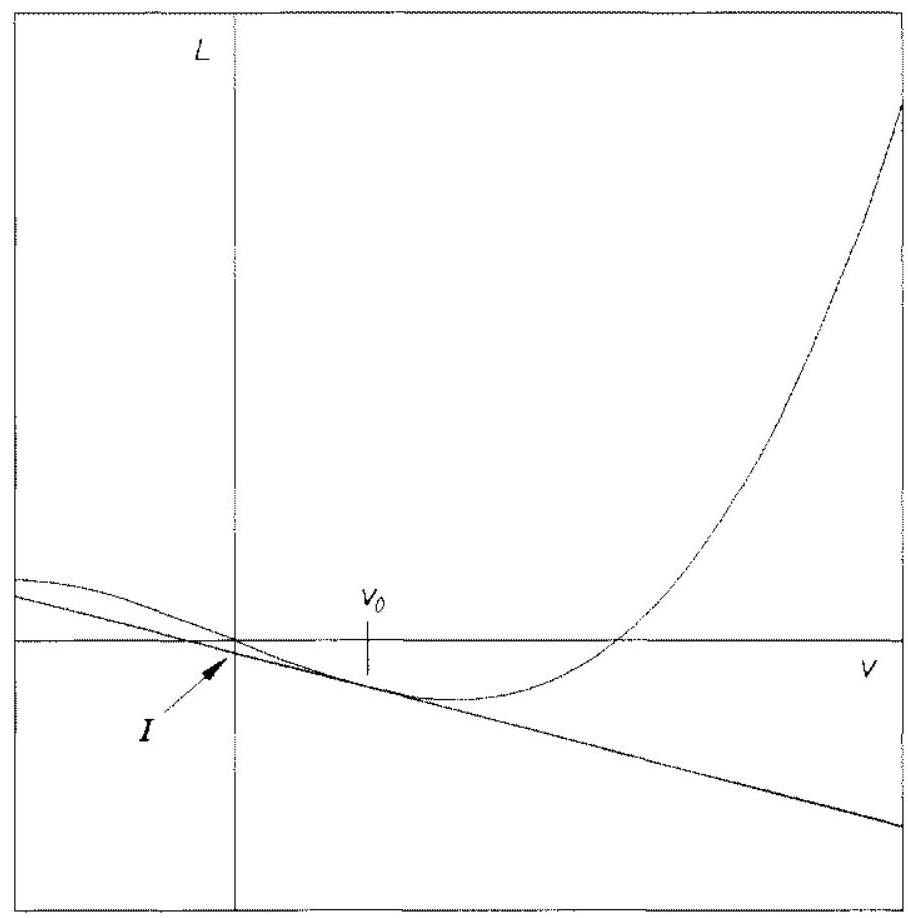
\includegraphics{Legen1.jpg}
  \caption[]{Una función $L(v)$, que tiene un punto de inflexión en el origen. La tangente a la curva en $v=v_{0}$ tiene pendiente $p=d L / d v$ calculada en $v_{0}$. La intersección en el eje $L$ se denomina $I$.}
  \labfig{fig:}
\end{marginfigure}

\begin{equation*}
  p(v) \equiv d L(v) / d v \tag{5.36}
\end{equation*}

\begin{definition}[Transformada de Legendre]
  La transformada de Legendre es una forma de describir la función o reproducir la gráfica enteramente en términos de $p$, sin referencia a $v$ : es decir, $p$ se convertirá en la variable independiente cuyos valores se utilizan para construir la curva. Pero del mismo modo que los valores de $v$ por sí solos, sin los valores de $L(v)$, no bastan para definir la curva, los valores de $p$ por sí solos tampoco bastan. Lo que se necesita es una función $H(p)$ de la nueva variable $p$.
\end{definition}


La función $H(p)$ se obtiene de la siguiente manera. Partimos de la Fig. 5.1, que muestra la tangente a la curva $L(v)$ en el punto $v=v_{0}$. La pendiente de esta tangente es $p\left(v_{0}\right) \equiv p_{0}$, y su intersección $I$ en el eje $L$ viene dado por

\[I=L\left(v_{0}\right)-p_{0} v_{0}\]

Hay una intersección diferente para cada $v$ en la curva (entonces eliminamos el subíndice 0 ), por lo que el intercepto se convierte en una función del punto $v$ y de la derivada $p$ en ese punto:
\begin{equation*}
  I(v, p)=L(v)-p v \tag{5.37}
  \end{equation*}

  Supongamos ahora que la Ec. (5.36) es invertible, de modo que $v$ puede obtenerse como función de $p$. En ese caso cada valor de $p$ determina unívocamente un valor de $v$ : una pendiente dada se da sólo en un punto de la curva. (La función de la Fig. 5.1 no cumple este requisito: la misma pendiente se da en más de un punto. Volveremos sobre esto más adelante). Cuando se encuentra $v(p)$, se puede sustituir por $v$ en (5.37), que se convierte entonces en una función de $p$ solamente. Entonces $H(p)$ se define por

  Hasta ahora $H(p)$ se ha obtenido a partir de $L(v)$. Ahora demostraremos que $L(v)$ puede obtenerse a partir de $H(p)$, y por tanto que las dos funciones son equivalentes. Primero lo demostraremos gráficamente y luego analíticamente.

  \begin{marginfigure}[]
    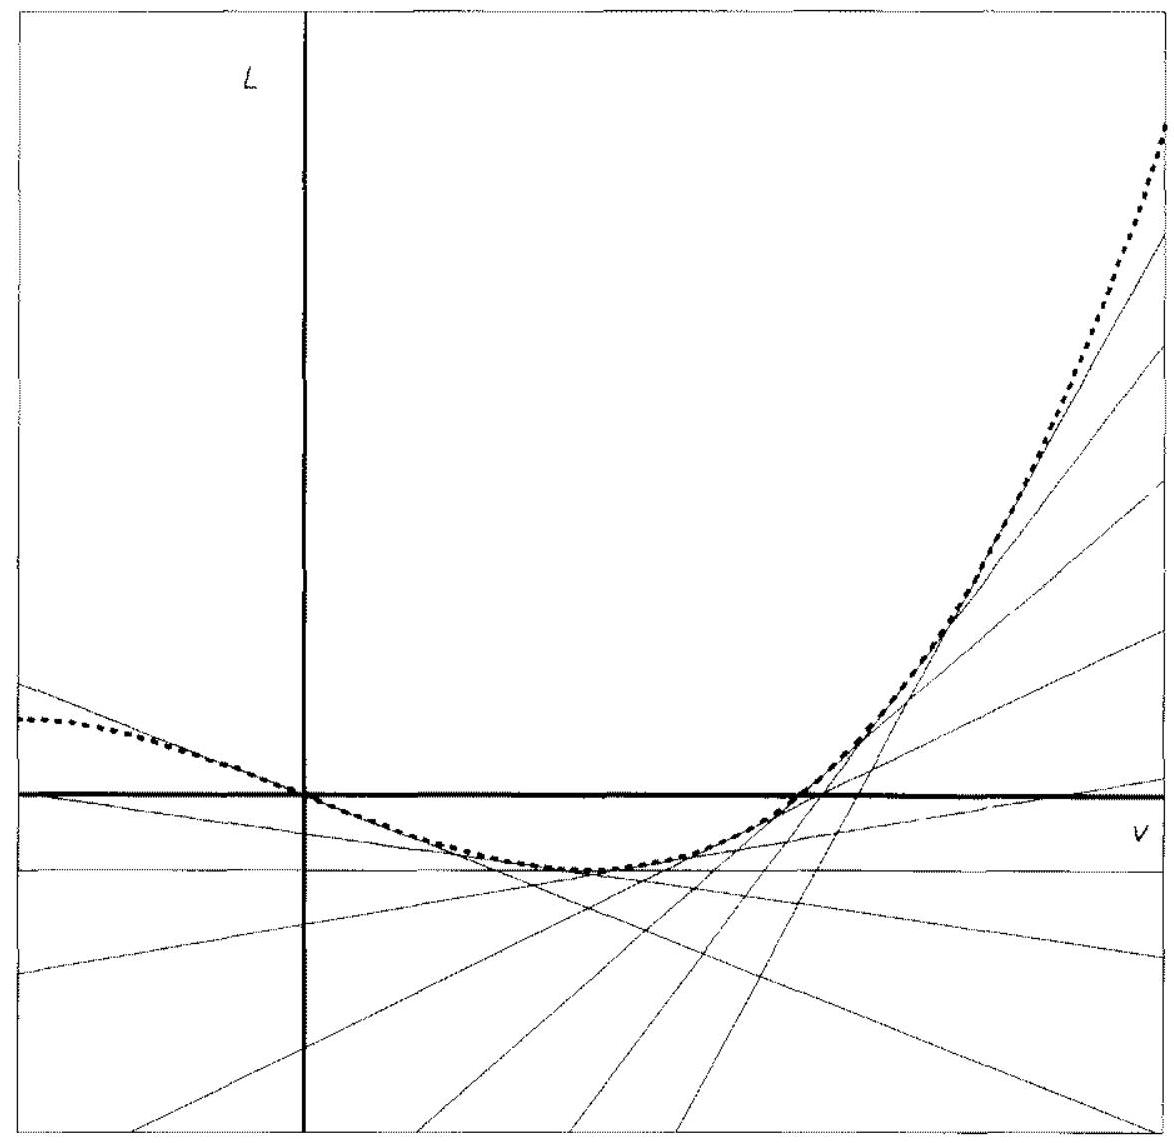
\includegraphics{Legen2.jpg}
    \caption[]{Tangentes a la curva $L(v)$ de la Fig. 5.1 para valores de $v$ por encima del punto de inflexión, obtenidas calculando ( $p, H(p)$ ) para varios valores de $p$. La curva punteada es $L(v)$, vista como la envolvente de las tangentes.}
    \labfig{fig:}
  \end{marginfigure}


  Supongamos que se conoce $H(p)$. Cada combinación $(p, H(p))$ corresponde a una recta de pendiente $p$ e intercepto $-H(p)$ sobre el eje $L$ en el plano $(L, v)$. El conjunto de tales rectas para $v>0$ (donde la relación entre $v$ y $p$ es única) en la Fig. 5.1 se muestra en la Fig. 5.2. La curva $L(v)$ es la envolvente de estas rectas, la curva continua tangente a todas ellas. Así pues, la curva $L(v)$ (o parte de ella) se ha construido a partir de $H(p)$.

  La prueba analítica requiere demostrar que la función $L(v)$ se puede obtener a partir de $H(p)$. Supongamos que se conoce $H(p)$ y tomemos la derivada de (5.38) con respecto a $p$ :

  \begin{equation*}
    \frac{d H}{d p}=v(p)+p \frac{d v}{d p}-\frac{d L}{d v} \frac{d v}{d p} \equiv v(p) \tag{5.39}
    \end{equation*}

    (use $d L / d v \equiv p$ ). El lado izquierdo es una función de $p$, por lo que (5.39) da $v$ como función de $p$. Supongamos ahora que esta ecuación puede invertirse para obtener la función $p(v)$, que puede utilizarse entonces para reescribir la Ec. (5.38) como función de v:

    \begin{equation*}
      L(v)=H(p(v))-p(v) v \tag{5.40}
      \end{equation*}

      La similitud de esta ecuación y (5.38) es sugerente: igual que $H$ da la representación pendiente-intersección de $L(v)$ en el plano $(v, L)$, $L$ da la representación pendiente-intersección de $H(p)$ en el plano $(p, H)$.


  Pasemos ahora a las condiciones de invertibilidad.


\begin{lemma}[Invertibilidad]
   Por definición cualquier función $p(v)$ da una $p$ única para cada valor de $v$; invertibilidad significa que $p(v)$ es una función uno a uno. Esto significa que $p(v)$ no pasa por un máximo ni por un mínimo, por lo que $d p / d v \neq 0$. Pero $d p / d v=d^{2} L / d v^{2}$, por lo que una condición necesaria para la invertibilidad es que la segunda derivada de $L$ no desaparezca: $L$ no debe tener punto de inflexión. (Análogamente, una condición necesaria para la invertibilidad de $v(p)$ es que $d^{2} H / d p^{2} \neq 0$). Esto puede verse también en las Figs. 5.1 y 5.2. Hay un punto de inflexión en el origen: $d^{2} L / d v^{2}=0$ en $v=0$. Si en la Fig. 5.2 se trazan tangentes a ambos lados de $v=0$, habrá más de un punto $v$ con la misma pendiente $p$, las rectas se superponen y el diagrama se vuelve irremediablemente confuso. Sin embargo, tanto a la derecha como a la izquierda de $v=0$, donde $v(p)$ es de un solo valor, el diagrama es claro.

   Para pasar a una dimensión superior, supongamos que $L(v)$ depende de una colección de $n$ variables $v=\left\{v^{1}, v^{2}, \ldots, v^{n}\right\}$. La demostración diagramática es mucho más difícil, pues las derivadas parciales $\partial L(v) / \partial v^{\alpha}=p_{\alpha}(v)$ dan la inclinación del hiperplano tangente en $v$, en lugar de la pendiente de la recta tangente. La hipersuperficie $L(v)$ en $n+1$ dimensiones es la envolvente de los hiperplanos tangentes. Analíticamente, sin embargo, el tratamiento procede en completa analogía con el caso de una sola variable, excepto que las condiciones necesarias para la invertibilidad ahora se convierten en que los Hessians $\partial^{2} L / \partial v^{\alpha} \partial v^{beta}$ y $\partial^{2} H / \partial p_{\alpha} \partial p_{\beta}$ sean no singulares (esto es de nuevo una manifestación del teorema de la función implícita).
\end{lemma}

\defbibnote{bibnote}{Aquí las referencias que ha usado Prado en clase.\par\bigskip} % Prepend this text to the bibliography
\printbibliography[heading=bibintoc, title=Bibliography, prenote=bibnote] % Add the bibliography heading to the ToC, set the title of the bibliography and output the bibliography note

\end{document}

